\documentclass[a4paper,oneside]{Tptesi2}

\usepackage[italian]{babel}
\usepackage{listings}
\usepackage{amsmath,amssymb}
\usepackage{verbatim}
\usepackage{indentfirst}
\usepackage[utf8]{inputenc}
\usepackage{subfigure}
\usepackage{algorithmic}
\usepackage{framed}
\usepackage{rotating}
\usepackage{cite}
\usepackage{url}
\def\UrlBreaks{\do\/\do-}
\usepackage{breakurl}
%\usepackage[breaklinks]{hyperref}

% Packages -----------------------------------------------------------------------
%\usepackage{amsthm}
%\usepackage{amsmath}          % Non necessario se usi TPTESI2 perche' gia` incluso
%\usepackage[dvips]{graphicx}  % Non necessario se usi TPTESI2 perche' gia` incluso
%\usepackage{url} %non usare se si usa hyperref

\newcommand{\mr}{\emph{motore di ricerca}}
\newcommand{\Mr}{\emph{Motore di ricerca}}
\newcommand{\ws}{Web~service }

\setcounter{tocdepth}{4} % per mostrare subsubsection in indice
%\setcounter{secnumdepth}{4} % per numerare anche subsubsection


% Use a small font for the verbatim environment
\makeatletter  % makes '@' an ordinary character
\renewcommand{\verbatim@font}{%
  \ttfamily\footnotesize\catcode`\<=\active\catcode`\>=\active%
}
\makeatother   % makes '@' a special symbol again
%
% Simboli Matematici -------------------------------------------------------------
%\newcommand{\h}{\mathcal{H}_\infty} % scorciatoia per sequenza usata spesso
% Definizioni & Teoremi ----------------------------------------------------------
\newtheorem{teorema}{Teorema}[chapter]
\newtheorem{corollario}[teorema]{Corollario}
\newtheorem{lemma}[teorema]{Lemma}
%\theoremstyle{definition}
\newtheorem{definizione}{Definizione}[chapter]
\newtheorem{proposizione}[definizione]{Proposizione}
% Formattazione Figure -----------------------------------------------------------
\setcounter{topnumber}{3}
\setcounter{totalnumber}{3}
\def\topfraction{1}
\def\textfraction{0}
% Fuzz ---------------------------------------------------------------------------
%\hfuzz10cm %Non scassare linee che escono dal bordo
% Frontespizio -------------------------------------------------------------------
       \title{Riconoscimento di oggetti in immagini termiche usando tecniche di augmentation}
       \author{Borsi Leonardo}
       \titolocorso{Ingegneria Informatica}
       \chair{Prof. Bertini Marco\\ }
       \numberofmembers{1} %numero dei relatori
       \degreeyear{2023/2024 }

%
% ---- Inclusioni (vedi piu` sotto per il comando "include" --------------
%\includeonly {introduzione,chapter1, chapter2}
%\includeonly {chapter1, chapter2, chapter3, chapter4, chapter5, chapter6}
%\includeonly{chapter6}
%
\hypersetup{%
%  pdfpagemode=FullScreen,%
  plainpages=false,%
  breaklinks,%
  pdftitle={},%
  pdfauthor={},%
  pdfsubject={},%
  pdfkeywords={},%
  colorlinks=false,
  hidelinks}

\begin{document}

\frontmatter

%\hyphenation{}
%
\pagestyle{headings} % rende attive le impostazioni sulla testata!
%
\maketitle % crea il frontespizio (ricordati di copiare "stemma.eps" nella tua directory)


\thispagestyle{empty}

{\fontfamily{ptm}\selectfont

    \begin{flushright}
    
    \textit{A Marga e Augusto,
    \\ per aver supportato ogni mia scelta,
    \\ seguendomi in ogni strada volessi imboccare,
    \\ per tutto ciò che mi avete trasmesso
    \\ e che continuate ad insegnarmi giorno per giorno}
    
    \vspace{0.7cm}
    
    \textit{A Martina e Niccolò,
    \\ per avermi sempre spronato ad essere la versione migliore di me stesso,
    \\ il fratello maggiore che vi meritate,
    \\ e per tutti i sorrisi strappati anche nei momenti più bui}
    
    \vspace{0.7cm}
    
    \textit{Ai due Luca, Benedetta e Marta,
    \\ per essere sempre stati il mio rifugio sicuro,
    \\ la famiglia che ti scegli e ti porti dietro per tutta la vita}
    
    \vspace{0.7cm}
    
    \textit{A Lorenzo, Filippo, Luca, Niccolò e Edoardo,
    \\ i migliori compagni d'avventura che potessi trovare,
    \\ per tutta la spensieratezza e la serenità che mi portate ogni giorno}
    
    \vspace{0.7cm}
    
    \textit{A Stefano,
    \\ per esser stato il mio mentore
    \\ ed aver creduto in me sin dal primo momento}
    
    \vspace{0.7cm}
    
    \textit{A Laura, Fausto, Concetta e Angelo,
    \\ per avermi reso l'uomo che sono oggi,
    \\ con tutto l'amore che continuate a darmi,
    \\ perfino da lassù}
    
    \end{flushright}
}





%
%
%\pagenumbering{roman}
\tableofcontents % inserisce indice generale
\cleardoublepage
%\addcontentsline{toc}{chapter}{Elenco delle figure}
%\listoffigures   % inserisce indice figure
%\addcontentsline{toc}{chapter}{Elenco delle tabelle}
%\listoftables    % inserisce indice tabelle
%\addcontentsline{toc}{chapter}{Elenco degli algoritmi}
%\listofalgorithms
%
%--------------- Inizio del testo vero e proprio
%

%\cleardoublepage
%\pagenumbering{arabic}

%\thispagestyle{empty}

{\fontfamily{ptm}\selectfont

    \begin{flushright}
    
    \textit{A Marga e Augusto,
    \\ per aver supportato ogni mia scelta,
    \\ seguendomi in ogni strada volessi imboccare,
    \\ per tutto ciò che mi avete trasmesso
    \\ e che continuate ad insegnarmi giorno per giorno}
    
    \vspace{0.7cm}
    
    \textit{A Martina e Niccolò,
    \\ per avermi sempre spronato ad essere la versione migliore di me stesso,
    \\ il fratello maggiore che vi meritate,
    \\ e per tutti i sorrisi strappati anche nei momenti più bui}
    
    \vspace{0.7cm}
    
    \textit{Ai due Luca, Benedetta e Marta,
    \\ per essere sempre stati il mio rifugio sicuro,
    \\ la famiglia che ti scegli e ti porti dietro per tutta la vita}
    
    \vspace{0.7cm}
    
    \textit{A Lorenzo, Filippo, Luca, Niccolò e Edoardo,
    \\ i migliori compagni d'avventura che potessi trovare,
    \\ per tutta la spensieratezza e la serenità che mi portate ogni giorno}
    
    \vspace{0.7cm}
    
    \textit{A Stefano,
    \\ per esser stato il mio mentore
    \\ ed aver creduto in me sin dal primo momento}
    
    \vspace{0.7cm}
    
    \textit{A Laura, Fausto, Concetta e Angelo,
    \\ per avermi reso l'uomo che sono oggi,
    \\ con tutto l'amore che continuate a darmi,
    \\ perfino da lassù}
    
    \end{flushright}
}






\frontmatter
\chapter{Introduzione}\label{ch:introduzione}

L'Object Detection è una delle aree più dinamiche ed importanti della Computer Vision, che mira ad individuare e classificare oggetti all'interno di un'immagine. Questa tecnologia trova applicazione in diversi settori, tra cui la sorveglianza, la guida autonoma e la robotica, dove è fondamentale riconoscere oggetti e persone in tempo reale e in condizioni variabili.

In particolare, le immagini termiche offrono un vantaggio significativo in situazioni di scarsa visibilità, come di notte o in condizioni atmosferiche avverse, permettendo di rilevare oggetti sulla base del calore che emettono. Tuttavia, lavorare con immagini termiche presenta delle sfide uniche, tra cui una minore risoluzione spaziale ed un minor contrasto rispetto alle immagini a luce visibile.

Questa tesi si propone di esplorare l'efficacia di diversi modelli di Object Detection applicati a immagini termiche e di migliorare le loro prestazioni attraverso l'uso di tecniche di Data Augmentation. Il lavoro sperimentale alla base di questa ricerca si concentra su tre tipologie di modelli YOLO: YOLOv8, YOLO-World e RT-DETR.

I primi tre capitoli della tesi forniscono una base teorica essenziale per comprendere le tecniche e le metodologie utilizzate, mentre il quarto capitolo è dedicato al lavoro sperimentale svolto con l'obiettivo di identificare il modello più efficiente nel riconoscimento di oggetti in immagini termiche.

\mainmatter
\chapter{Object Detection}\label{ch:object-detection}

\section{Il Problema dell'Object Detection}

\subsection{Computer Vision}
La Computer Vision è una branca dell'intelligenza artificiale che si occupa dello sviluppo di metodi che consentano ai computer di interpretare e comprendere il mondo visivo in modo simile agli esseri umani. Questa capacità è cruciale per sviluppare applicazioni avanzate che richiedono l'analisi e l'elaborazione delle immagini e dei video. La Computer Vision comprende quindi le basi teoriche, gli algoritmi e i modelli matematici necessari per acquisire, elaborare, analizzare e comprendere le immagini digitali, con l'obiettivo di estrarre informazioni significative dall'ambiente visivo.

Tra i problemi centrali di cui si occupa la Computer Vision, troviamo:
\begin{itemize}
  \item \textbf{Image Recognition}: Identificare e classificare oggetti o scene all'interno di un'immagine. Questo include compiti come il riconoscimento facciale, il riconoscimento di oggetti e il riconoscimento di azioni.
  \item \textbf{Object Detection}: Localizzare e identificare oggetti di interesse all'interno di un'immagine, determinando la loro posizione attraverso bounding box. Questo è fondamentale per applicazioni come il tracciamento degli oggetti, la guida autonoma e la sorveglianza.
  \item \textbf{Semantic Segmentation}: Dividere un'immagine in segmenti che corrispondono a oggetti o regioni con caratteristiche simili. Questo aiuta a comprendere la struttura dell'immagine a livello di pixel.
  \item \textbf{Scene Recognition}: Interpretare e descrivere l'intera scena rappresentata in un'immagine, inclusi gli oggetti presenti e le loro relazioni spaziali.
  \item \textbf{Pose Estimation}: Determinare la posizione e l'orientamento di un oggetto nello spazio tridimensionale a partire da immagini bidimensionali.
  \item \textbf{3D Reconstruction}: Ricostruire modelli tridimensionali di oggetti o scene a partire da immagini bidimensionali. Questo è cruciale per applicazioni come la realtà aumentata e la robotica.
  \item \textbf{Object Tracking}: Seguire il movimento di uno o più oggetti attraverso una sequenza di immagini o video. Questo è essenziale per applicazioni come la sorveglianza video e la guida autonoma.
  \item \textbf{Super-Resolution}: Migliorare la risoluzione di un'immagine partendo da versioni a bassa risoluzione, utile per migliorare la qualità visiva e per analisi più dettagliate.
\end{itemize}

Questi problemi sono alla base di molte applicazioni pratiche della Computer Vision e sono spesso interconnessi.


\subsection{Object Detection}
L'Object Detection è quindi uno dei problemi fondamentali della Computer Vision. Esso riguarda la localizzazione e identificazione di uno o più oggetti di interesse all'interno di un'immagine o di un video. A differenza dell'Image Recognition, che si limita a classificare un'intera immagine, l'Object Detection deve determinare sia la presenza degli oggetti sia le loro posizioni precise.

\begin{figure}[ht]
    \centering
    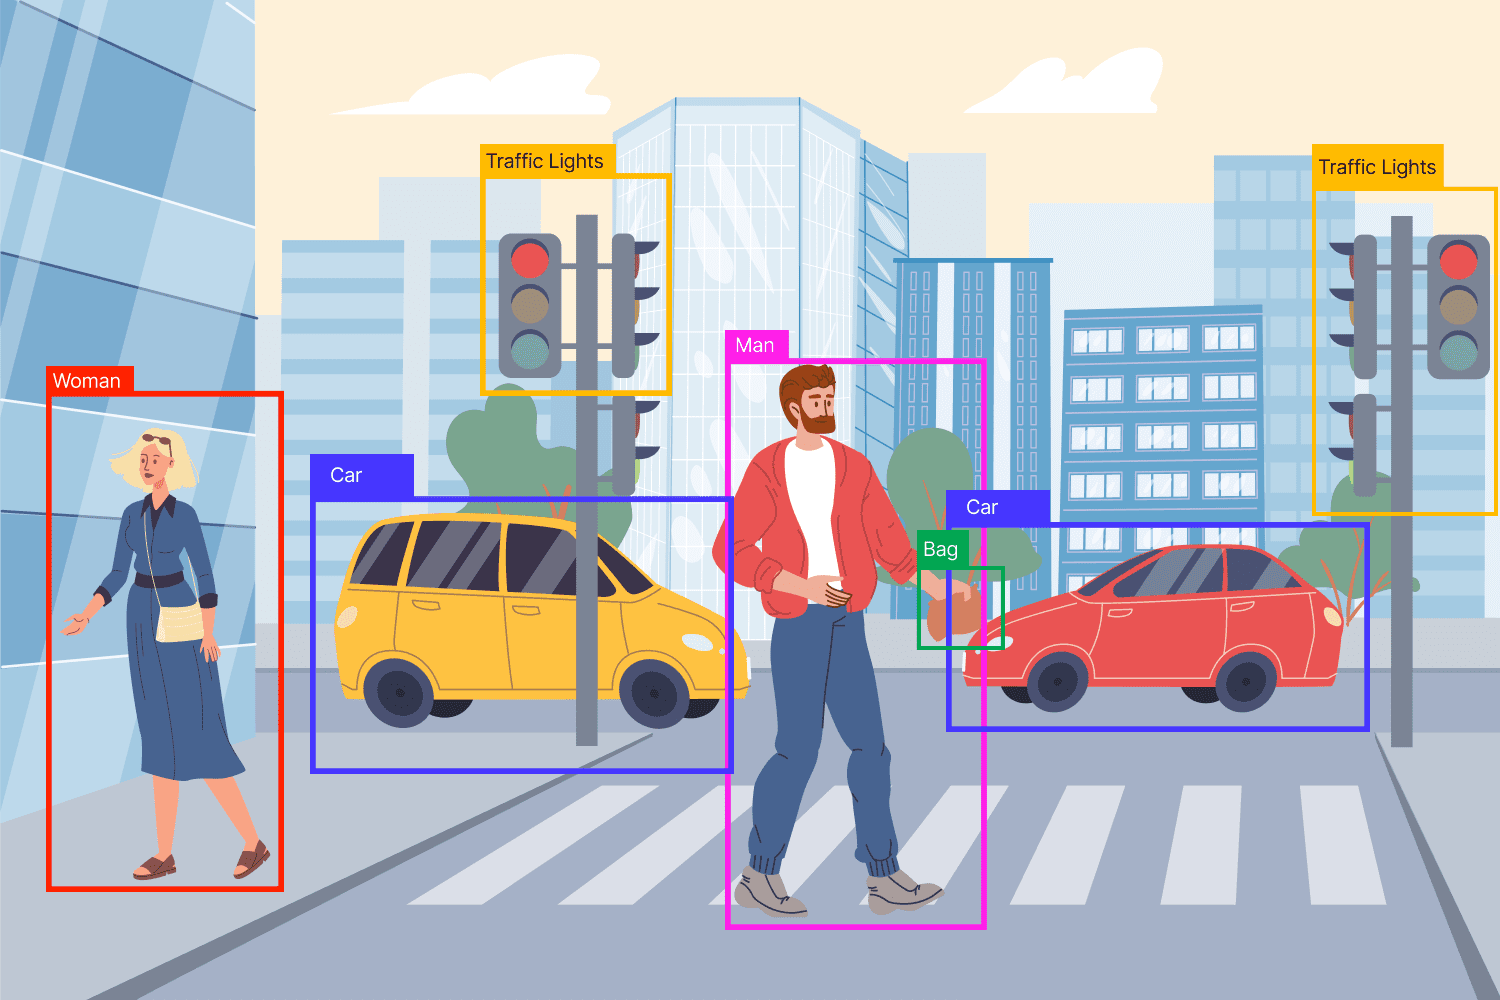
\includegraphics[width=0.75\textwidth]{files/capitoli/1-object-detection/assets/object-detection-example.png}
    \caption{\label{fig:object-detection-example}Esempio di Object Detection di un'immagine\cite{1}}
\end{figure}

L'Object Detection ha due obiettivi principali:
\begin{itemize}
  \item \textbf{Localizzazione}: Determinare la posizione degli oggetti all'interno dell'immagine, solitamente rappresentata da bounding box (rettangoli che contornano gli oggetti).
  \item \textbf{Classificazione}: Identificare la classe a cui appartiene ogni oggetto rilevato (ad esempio persona, automobile, animale, ecc...).
\end{itemize}

Questi obiettivi richiedono algoritmi capaci di elaborare immagini complesse e di generare previsioni accurate e efficienti in termini di calcolo.

L'Object Detection è pertanto un processo complesso che combina diverse fasi, ognuna delle quali gioca un ruolo cruciale nel garantire l'accuratezza e l'efficienza del sistema complessivo.

I principali passaggi coinvolti nell'Object Detection sono:
\begin{itemize}
  \item \textbf{Feature Extraction}
  \item \textbf{Bounding Box Prediction}
  \item \textbf{Classification}
  \item \textbf{Non-Maximum Suppression (NMS)}
\end{itemize}

\subsubsection{Feature Extraction}
La fase di Feature Extraction è cruciale nell'Object Detection, in quanto le caratteristiche estratte rappresentano la base su cui si fondano le successive fasi di localizzazione e classificazione. Questa fase coinvolge l'uso di reti neurali convoluzionali (CNN) per identificare caratteristiche rilevanti delle immagini, come bordi, texture, forme e colori.

\begin{figure}[ht]
    \centering
    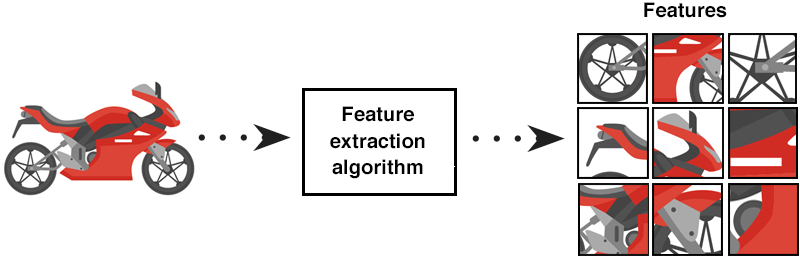
\includegraphics[width=1\textwidth]{files/capitoli/1-object-detection/assets/feature-extraction.png}
    \caption{\label{fig:feature-extraction}Esempio di Feature Extraction di un'immagine\cite{2}}
\end{figure}

\newpage

Le CNN sono una classe di reti neurali composte da vari layer di diversi tipi, ciascuno con una funzione specifica:
\begin{itemize}
  \item \textbf{Convolutional Layers}: estraggono caratteristiche locali come bordi, angoli e texture tramite l'applicazione di filtri (kernel) sull'immagine di input. Ogni kernel convoluziona l'immagine generando una feature map che evidenzia la presenza di specifici pattern.
  \item \textbf{Activation Layers}: applicano una funzione di attivazione non lineare (ad esempio, ReLU - Rectified Linear Unit) dopo ogni convolutional layer, la quale introduce non-linearità nel modello, permettendo alla rete di apprendere rappresentazioni più complesse.
  \item \textbf{Pooling Layers}: riducono le dimensioni spaziali delle feature map (tipicamente mediante operazioni di max pooling o average pooling), riducendo così il numero di parametri e computazioni nella rete, e introducendo invarianza rispetto alle traslazioni. Questo aiuta a rendere il modello più robusto e a prevenire l'overfitting.
\end{itemize}

\begin{figure}[ht]
    \centering
    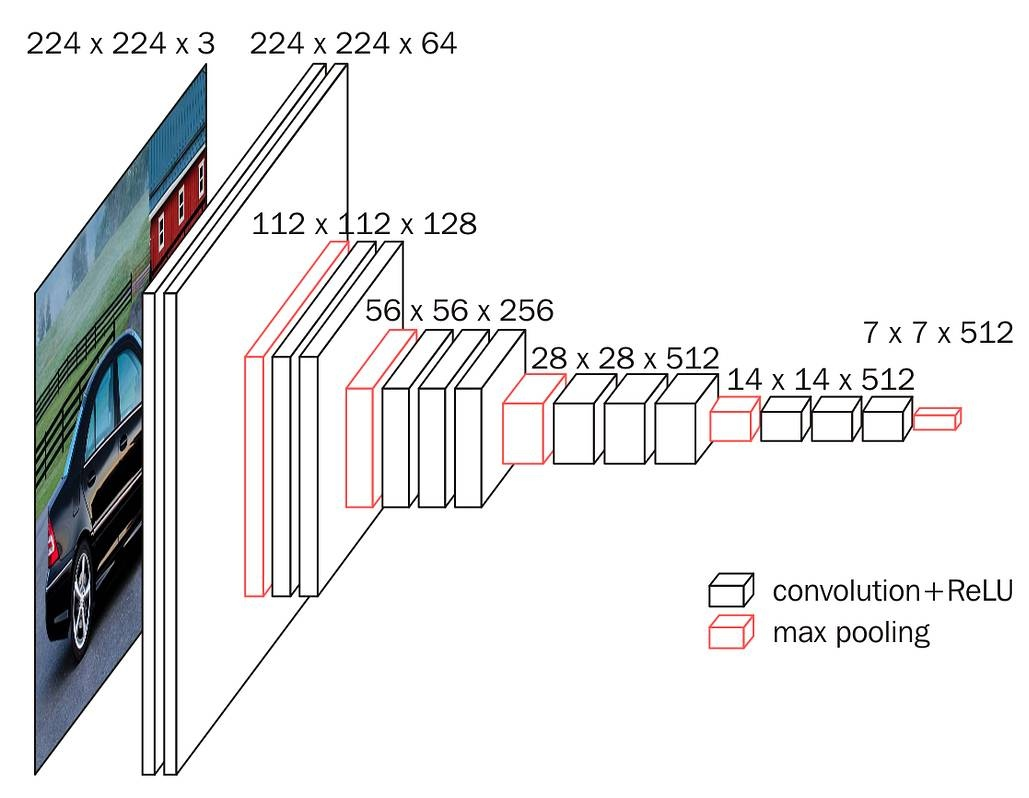
\includegraphics[width=0.6\textwidth]{files/capitoli/1-object-detection/assets/feature-extraction-layers.jpg}
    \caption{\label{fig:feature-extraction-layers}Layers della CNN adibiti alla Feauture Extraction\cite{3}}
\end{figure}

Quando un'immagine viene data in input ad una CNN, questa passa attraverso la serie di convolutional e pooling layers. I primi convolutional layers tendono a rilevare caratteristiche di basso livello, come bordi e texture, mentre i successivi catturano caratteristiche di livello più alto, come parti di oggetti e forme complete. L'uso di multipli convolutional layers permette quindi alla rete di costruire una rappresentazione gerarchica delle caratteristiche dell'immagine.

Il risultato finale della fase di Feature Extraction è una serie di feature maps che catturano informazioni spaziali e di contesto sull'immagine. Queste feature maps sono poi utilizzate nei passaggi successivi per la predizione delle bounding box e la classificazione degli oggetti.

\subsubsection{Bounding Box Prediction e Classification}
La predizione delle bounding box e la classificazione degli oggetti sono due passaggi cruciali nell'Object Detection. A seconda dell'architettura del modello, questi passaggi possono essere eseguiti separatamente o simultaneamente.

Nei modelli basati su region proposals, come R-CNN e le sue varianti, la predizione delle bounding box e la classificazione avvengono in due passaggi distinti:

\begin{enumerate}
  \item \textbf{Generazione delle Proposal Regions}: in questa fase, il modello utilizza algoritmi come il Selective Search o una Region Proposal Network (RPN) per generare un insieme di region proposals, che sono regioni dell'immagine candidate a contenere oggetti. Il Selective Search utilizza tecniche di segmentazione per trovare regioni simili, mentre l'RPN è una rete neurale che produce direttamente proposte di regioni.

\begin{figure}[ht]
    \centering
    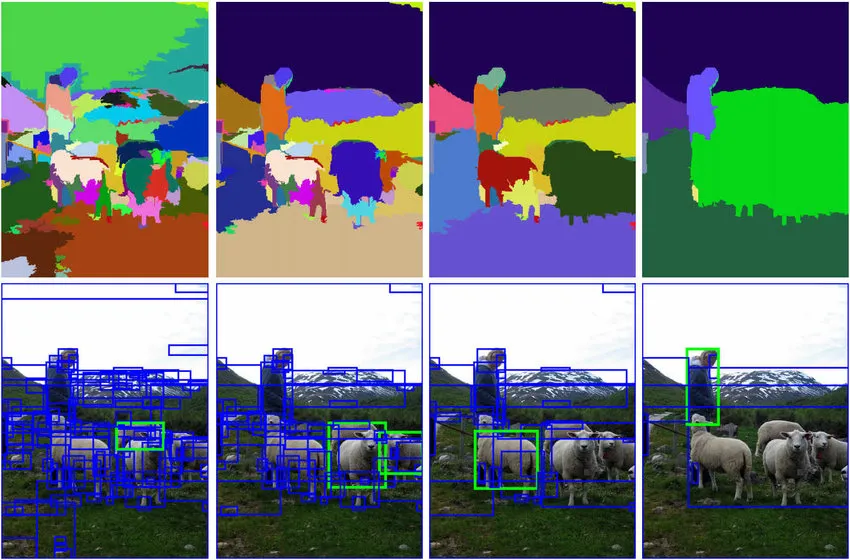
\includegraphics[width=0.8\textwidth]{files/capitoli/1-object-detection/assets/selective-search-region-proposals.png}
    \caption{\label{fig:selective-search-region-proposals}Esempio di generazione delle Proposal Regions con l'algoritmo Selective Search\cite{4}}
\end{figure}
  
  \item \textbf{Predizione delle Bounding Box e Classificazione}: ogni region proposal viene estratta dalle feature maps e passata attraverso una CNN che effettua la predizione delle bounding box precise e la classificazione degli oggetti. In R-CNN, questo passaggio viene eseguito separatamente per ciascuna region proposal, mentre in varianti come Fast R-CNN e Faster R-CNN, queste operazioni vengono ottimizzate per migliorare la velocità e l'efficienza.
\end{enumerate}

Nei modelli single-shot, come SSD e YOLO, la predizione delle bounding box e la classificazione degli oggetti avvengono simultaneamente in un unico passaggio.

Questo approccio è caratterizzato dai seguenti passaggi chiave:
\begin{enumerate}
  \item \textbf{Suddivisione in Griglia}: dopo la feature extraction, l'immagine di input viene suddivisa in una griglia di dimensioni predefinite, ad esempio 7x7 o 13x13, a seconda delle specifiche del modello.
  \item \textbf{Predizione delle Bounding Box}: per ogni cella della griglia, il modello utilizza le feature maps per predirre un insieme di bounding box, ciascuna definita da:
  \begin{itemize}
    \item Coordinate (x, y) del centro della bounding box rispetto alla cella della griglia
    \item Altezza e larghezza (h, w) della bounding box, normalizzate rispetto alle dimensioni dell'immagine
    \item Un punteggio di confidenza (objectness score) che riflette la probabilità che la bounding box contenga un oggetto e la precisione con cui la bounding box delimita l'oggetto
  \end{itemize}
  \item \textbf{Classificazione}: oltre alle coordinate e all'objectness score, per ogni bounding box viene predetta una distribuzione di probabilità sulle classi degli oggetti. Il modello quindi stima la probabilità che l'oggetto contenuto nella bounding box appartenga a ciascuna delle classi target.
  \item \textbf{Calcolo del Punteggio Finale}: l'objectness score per ogni bounding box viene moltiplicato per le probabilità di classe per ottenere un punteggio finale per ogni combinazione di bounding box e classe. Questo punteggio finale aiuta a determinare quali bounding box e classi saranno considerate nella fase finale di rilevamento.
\end{enumerate}

\begin{figure}[ht]
    \centering
    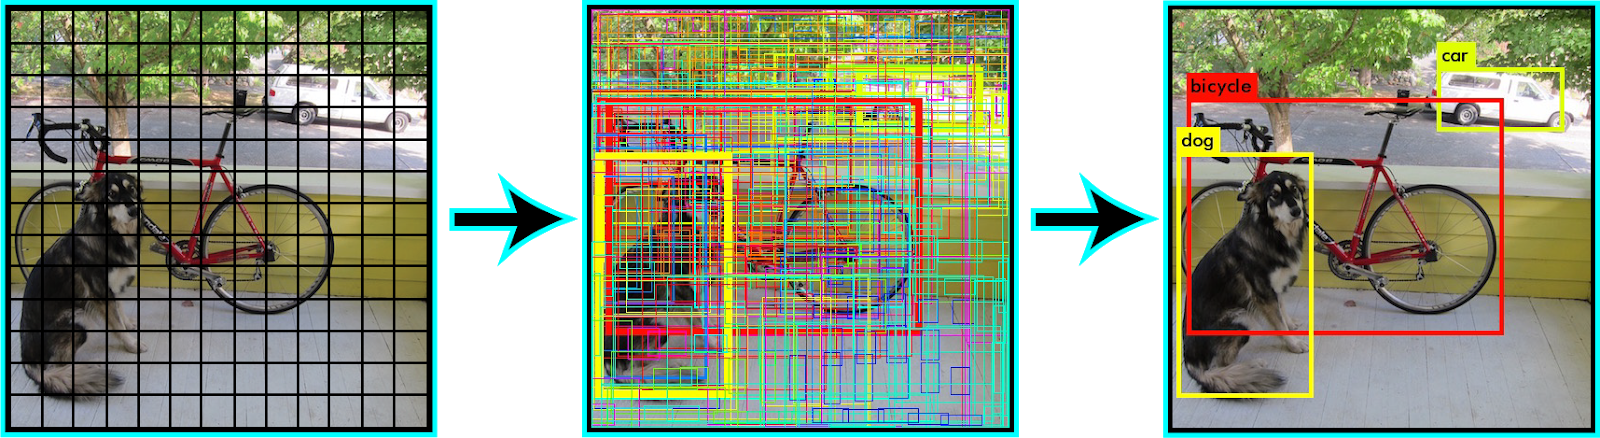
\includegraphics[width=0.8\textwidth]{files/capitoli/1-object-detection/assets/single-shot-grid.png}
    \caption{\label{fig:single-shot-grid}Bounding Box Prediction e Classification dei modelli single-shot\cite{5}}
\end{figure}


\newpage

\subsubsection{Non-Maximum Suppression}
La Non-Maximum Suppression (NMS) è una tecnica essenziale utilizzata nei modelli di Object Detection per ridurre le proposte ridondanti di bounding box o regioni che coprono gli oggetti rilevati. 
Questa viene applicata dopo la fase di generazione delle proposte (bounding box o regioni), le quali vengono valutate e ordinate in base a un punteggio di confidenza, che rappresenta la probabilità che una proposta contenga un oggetto.

L'NMS identifica e rimuove le proposte che hanno un'elevata sovrapposizione con altre proposte di punteggio più alto, mantenendo solo quelle più accurate e significative.

\begin{figure}[ht]
    \centering
    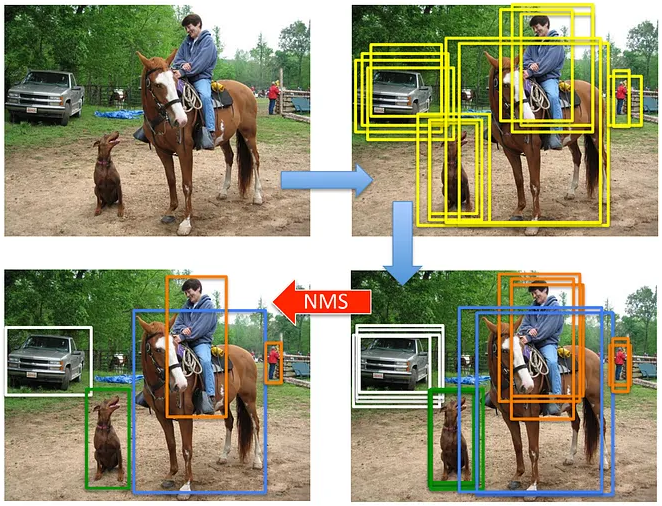
\includegraphics[width=0.7\textwidth]{files/capitoli/1-object-detection/assets/nms-example.png}
    \caption{\label{fig:nms-example}Esempio di rimozione delle bounding box ridondanti tramite Non-Maximum Suppression\cite{5}}
\end{figure}

\newpage

\section{Modelli per l'Object Detection}

Nel campo dell'Object Detection, vari modelli hanno rivoluzionato il rilevamento degli oggetti nelle immagini, contribuendo significativamente alla precisione e all'efficienza di questa tecnologia fondamentale della Computer Vision. Ogni modello presenta un approccio distintivo per affrontare le sfide di localizzazione e classificazione degli oggetti.

\subsection{R-CNN e Varianti}

\subsubsection{R-CNN}
R-CNN (Region-based Convolutional Neural Network) è stato uno dei primi modelli ad adottare un approccio basato sulle region proposals per l'Object Detection. Proposto da Ross Girshick, Jeff Donahue, Trevor Darrell e Jitendra Malik nel 2014 \cite{6}, ha segnato un punto di svolta nell'utilizzo delle reti neurali convoluzionali per il rilevamento degli oggetti. Prima dell'introduzione di R-CNN, i metodi tradizionali per l'Object Detection erano basati su tecniche di estrazione di features manuali e classificatori separati. Questi approcci erano spesso limitati dalla necessità di progettare manualmente le features e dalla loro mancanza di robustezza e generalizzazione.

R-CNN si distingue per il suo approccio in tre fasi visto precedentemente:

\begin{enumerate}
    \item \textbf{Generazione delle Proposal Regions}: genera un insieme di proposal regions candidate tramite algoritmi come il Selective Search, le quali vengono poi selezionate in base a caratteristiche di basso livello come colore, texture e forma.
    \item \textbf{Feature Extraction}: ogni proposal region viene trasformata in una dimensione fissa e passata attraverso una rete convoluzionale pre-addestrata, come AlexNet o VGG-16. Questo processo genera una feature map per ciascuna region proposal, catturando le informazioni rilevanti dell'area proposta.
    \item \textbf{Classificazione e Ottimizzazione delle Bounding Box}: le feature estratte da ciascuna region proposal vengono fornite a un classificatore SVM per determinare la presenza di oggetti e per la classificazione, mentre un regressore lineare ottimizza le coordinate della bounding box prevista per migliorare la precisione della localizzazione dell'oggetto.
\end{enumerate}

\begin{figure}[ht]
    \centering
    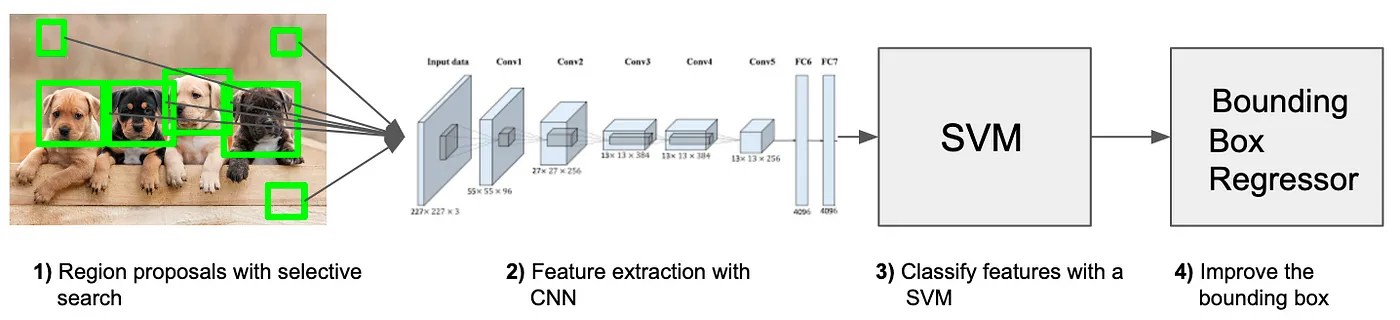
\includegraphics[width=1\textwidth]{files/capitoli/1-object-detection/assets/r-cnn.png}
    \caption{\label{fig:r-cnn}Architettura di R-CNN\cite{7}}
\end{figure}

\vspace{1.7cm}

\subsubsection{Fast R-CNN}
Fast R-CNN, proposto da Ross Girshick nel 2015\cite{8}, migliora l'efficienza di R-CNN introducendo le seguenti migliorie:

\begin{itemize}
    \item \textbf{Utilizzo di una sola CNN}: integra l'intero processo di rilevamento degli oggetti in una singola rete, combinando l'estrazione di features e la generazione di region proposals
    \item \textbf{RoI Pooling}: introduce la tecnica di RoI (Region of Interest) pooling per estrarre features dalle feature map generate, gestendo efficacemente regioni di dimensioni variabili.
\end{itemize}

\begin{figure}[ht]
    \centering
    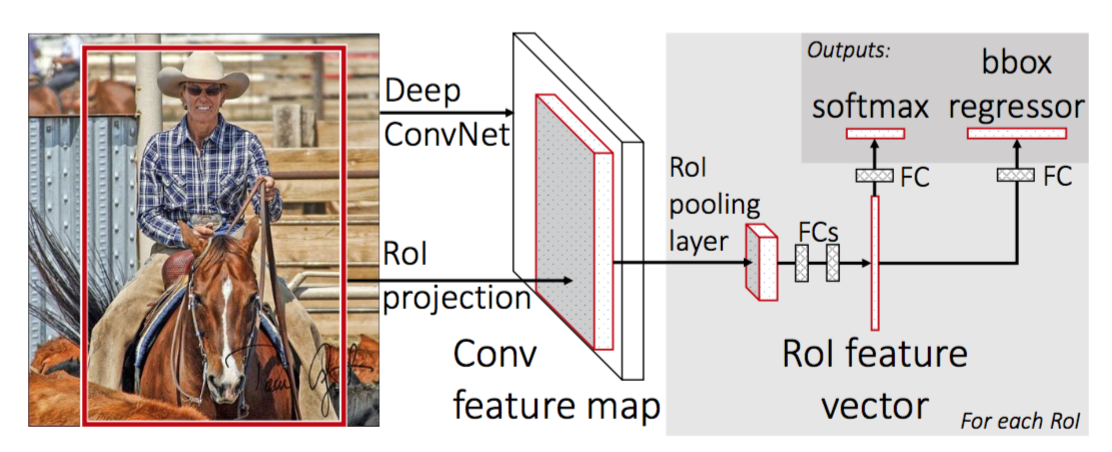
\includegraphics[width=0.8\textwidth]{files/capitoli/1-object-detection/assets/fast-r-cnn.png}
    \caption{\label{fig:fast-r-cnn}Architettura di Fast R-CNN\cite{9}}
\end{figure}

\vspace{1.6cm}

\subsubsection{Faster R-CNN}
Faster R-CNN, proposto da Shaoqing Ren, Kaiming He, Ross Girshick e Jian Sun nel 2016\cite{10}, rappresenta un ulteriore miglioramento rispetto a Fast R-CNN, introducendo un approccio più efficiente per la generazione delle region proposals. Principali migliorie: 

\begin{itemize}
    \item \textbf{Region Proposal Network (RPN)}: introduce una RPN che opera condividendo la feature map con la rete principale, permettendo la generazione di proposte di regioni in modo efficiente e integrato.
    \item \textbf{Architettura two-stage}: divide il processo di rilevamento degli oggetti in due fasi: prima, il RPN propone regioni d'interesse basate sulla feature map condivisa; successivamente, queste proposte vengono elaborate da un classificatore e un regressore per la classificazione degli oggetti e l'ottimizzazione delle bounding box.
    \item \textbf{RoI Pooling migliorato}: implementa un RoI pooling migliorato all'interno dell'RPN e nella fase successiva di elaborazione delle proposte. Questo approccio ottimizza la gestione delle regioni di interesse, migliorando la precisione complessiva del rilevamento degli oggetti.
\end{itemize}

\begin{figure}[ht]
    \centering
    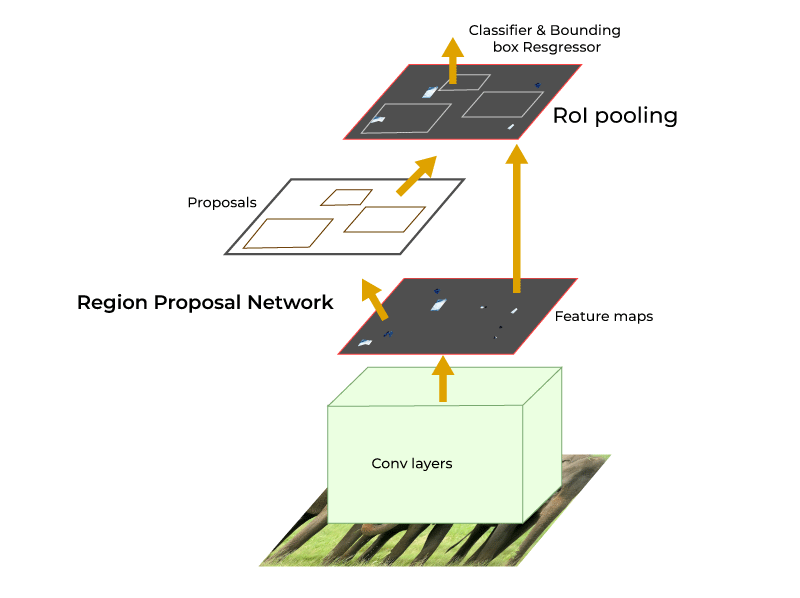
\includegraphics[width=0.8\textwidth]{files/capitoli/1-object-detection/assets/faster-r-cnn.png}
    \caption{\label{fig:faster-r-cnn}Architettura di Faster R-CNN\cite{9}}
\end{figure}

\newpage

\subsection{SSD}
Il modello SSD (Single Shot MultiBox Detector) è stato un importante avanzamento nell'ambito dell'Object Detection. Proposto da Wei Liu, Dragomir Anguelov, Dumitru Erhan, Christian Szegedy, Scott Reed, Cheng-Yang Fu e Alexander C. Berg nel 2016\cite{11}, ha introdotto un approccio single-shot per il rilevamento degli oggetti, combinando predizione delle bounding box e classificazione degli oggetti in un unico passaggio. Prima dell'SSD, i modelli two-stage come R-CNN e le sue varianti dominavano il campo, con una fase separata di generazione delle region proposals seguita dalla classificazione. Questi approcci, sebbene accurati, erano spesso limitati dalla complessità computazionale e dalla lentezza del processo.
Eliminando questa fase separata adottata dai modelli two-stage, rende il processo di rilevamento più rapido ed efficiente. Questa caratteristica ha reso SSD ideale per applicazioni che richiedono un'elaborazione veloce delle immagini, come la videosorveglianza e i sistemi di guida autonoma.

\begin{figure}[ht]
    \centering
    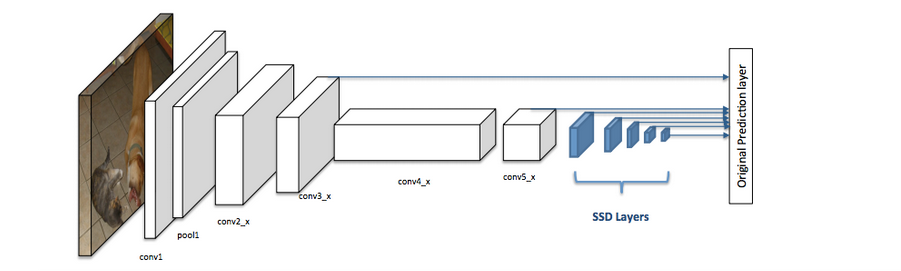
\includegraphics[width=0.95\textwidth]{files/capitoli/1-object-detection/assets/ssd.png}
    \caption{\label{fig:ssd}Architettura di SSD\cite{12}}
\end{figure}

Un'altra innovazione chiave di SSD è l'utilizzo delle \textbf{anchor box}: bounding box con dimensioni predefinite disposte su una griglia che suddivide l'immagine. Durante l'addestramento, SSD predice l'offset rispetto a ciascuna anchor box per adattare la posizione e le dimensioni della bounding box alle caratteristiche specifiche dell'oggetto da rilevare.

Questo approccio consente a SSD di individuare oggetti di diverse dimensioni e forme con maggiore accuratezza e robustezza.

\begin{figure}[ht]
    \centering
    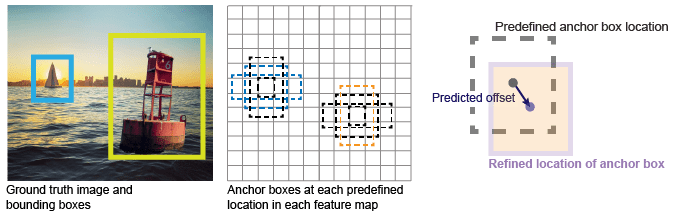
\includegraphics[width=1\textwidth]{files/capitoli/1-object-detection/assets/ssd-anchors.png}
    \caption{\label{fig:ssd-anchors}Utilizzo delle anchor box nell'SSD\cite{13}}
\end{figure}

SSD rappresenta quindi un passo significativo verso modelli più efficienti e versatili per l'Object Detection, combinando alta precisione con prestazioni ottimali in tempo reale.

\subsection{YOLO}
Il modello YOLO (You Only Look Once) rappresenta un'altra pietra miliare nell'ambito dell'Object Detection, affiancandosi all'SSD come uno dei primi modelli single-shot a rivoluzionare il campo. Proposto originariamente da Joseph Redmon, Santosh Divvala, Ross Girshick e Ali Farhadi nel 2016\cite{14}, YOLO segue l'approccio innovativo che combina la predizione delle bounding box e la classificazione degli oggetti in un singolo passaggio. Come nell'SSD, l'immagine viene suddivisa in una griglia e vengono predette bounding box e probabilità di classe direttamente per ciascuna cella della griglia.

YOLO si distingue per la sua capacità di considerare il contesto globale dell'immagine durante il processo di rilevamento. Ogni cella della griglia non solo predice le bounding box ma valuta anche la confidenza di ciascuna predizione in relazione a tutte le altre predizioni nell'immagine. Questo approccio globale contribuisce a migliorare la coerenza e la precisione complessiva del modello.

Inoltre, YOLO utilizza un'unica CNN per l'intero processo di rilevamento degli oggetti, semplificando ulteriormente l'architettura e migliorando l'efficienza computazionale. Questa caratteristica lo rende particolarmente adatto per dispositivi con risorse limitate e per applicazioni embedded.

\begin{figure}[ht]
    \centering
    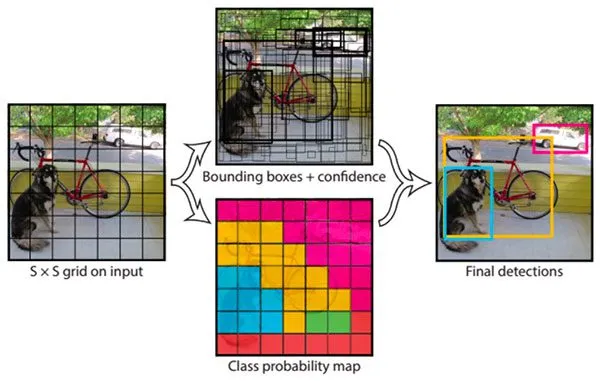
\includegraphics[width=0.8\textwidth]{files/capitoli/1-object-detection/assets/yolo.png}
    \caption{\label{fig:yolo}Object Detection tramite YOLO\cite{15}}
\end{figure}

YOLO ha trovato ampio impiego in una vasta gamma di applicazioni, dalla videosorveglianza alla guida autonoma, grazie alla sua velocità, precisione e capacità di gestire oggetti di diverse dimensioni e forme all'interno di un'immagine.

\newpage


\section{Applicazioni dell'Object Detection}

L'object detection è una tecnologia fondamentale con numerose applicazioni pratiche in vari settori, quali:
\begin{enumerate}
    \item \textbf{Sicurezza e Sorveglianza}: utilizzata per monitorare ambienti e individuare attività sospette. Esempi includono il rilevamento di persone, veicoli o oggetti non autorizzati in aree sensibili come aeroporti, banche e stazioni ferroviarie.
    \item \textbf{Automazione Industriale}: usata per il controllo di qualità, l'ispezione automatizzata dei prodotti e la gestione degli inventari.
    \item \textbf{Guida Autonoma e Veicoli Intelligenti}: consente ai veicoli di rilevare e reagire in tempo reale a pedoni, veicoli, segnaletica stradale e altri ostacoli.
    \item \textbf{Sanità e Medicina}: supporta la diagnostica medica automatizzata, il monitoraggio dei pazienti e la ricerca scientifica.
    \item \textbf{Commercio e Marketing}: impiegata per migliorare l'esperienza del cliente, ottimizzare la gestione del magazzino e analizzare il comportamento dei consumatori, tramite l'analisi delle immagini e dei video permette di monitorare gli scaffali nei negozi e di rilevare automaticamente il movimento dei prodotti.
    \item \textbf{Sicurezza Stradale e Controllo del Traffico}: fondamentale per il miglioramento della sicurezza stradale e l'ottimizzazione del controllo del traffico urbano, grazie a sistemi avanzati che possono rilevare incidenti, monitorare il flusso veicolare, riconoscere targhe di registrazione e applicare le normative stradali.
\end{enumerate}

\chapter{YOLO}\label{ch:yolo}

\section{You Only Look Once}

Il nome "You Only Look Once" deriva dalla filosfia di design che sta alla base del modello ideato da Joseph Redmon, Santosh Divvala, Ross Girshick e Ali Farhadi nel 2016\cite{14}: l'immagine deve essere elaborata una sola volta per effettuare sia la predizione delle bounding box che la classificazione degli oggetti. A differenza dei modelli two-stage, che richiedono un primo passaggio per generare le region proposals e un secondo passaggio per classificarle, YOLO effettua tutto in un unico passo. Questo approccio consente di ridurre drasticamente il tempo di elaborazione e semplifica l'architettura complessiva del modello.

Esistono quindi alcuni principi chiave che hanno influenzato il design e lo sviluppo del modello:
\begin{itemize}
  \item \textbf{Approccio Globale all'Immagine}: A differenza dei modelli precedenti che esaminano porzioni dell'immagine in sequenza, YOLO considera l'intera immagine in un singolo passaggio. Questo consente al modello di avere una visione globale del contesto, riducendo la probabilità di predizioni incoerenti tra le diverse regioni dell'immagine.
  \item \textbf{Efficienza Computazionale}: YOLO è progettato per essere estremamente veloce. L'approccio single-shot consente di ridurre drasticamente il tempo di elaborazione, rendendolo adatto per applicazioni in tempo reale come la videosorveglianza, la guida autonoma e altre situazioni dove la velocità è critica.
  \item \textbf{Semplicità e Generalizzazione}:  La semplicità dell'architettura di YOLO non solo facilita l'implementazione, ma migliora anche la capacità del modello di generalizzare su diverse tipologie di immagini e scenari. Utilizzando un'unica rete neurale convoluzionale per predire sia le bounding box che le probabilità di classe, YOLO riesce a mantenere un equilibrio tra complessità e prestazioni.
\end{itemize}

\begin{figure}[ht]
    \centering
    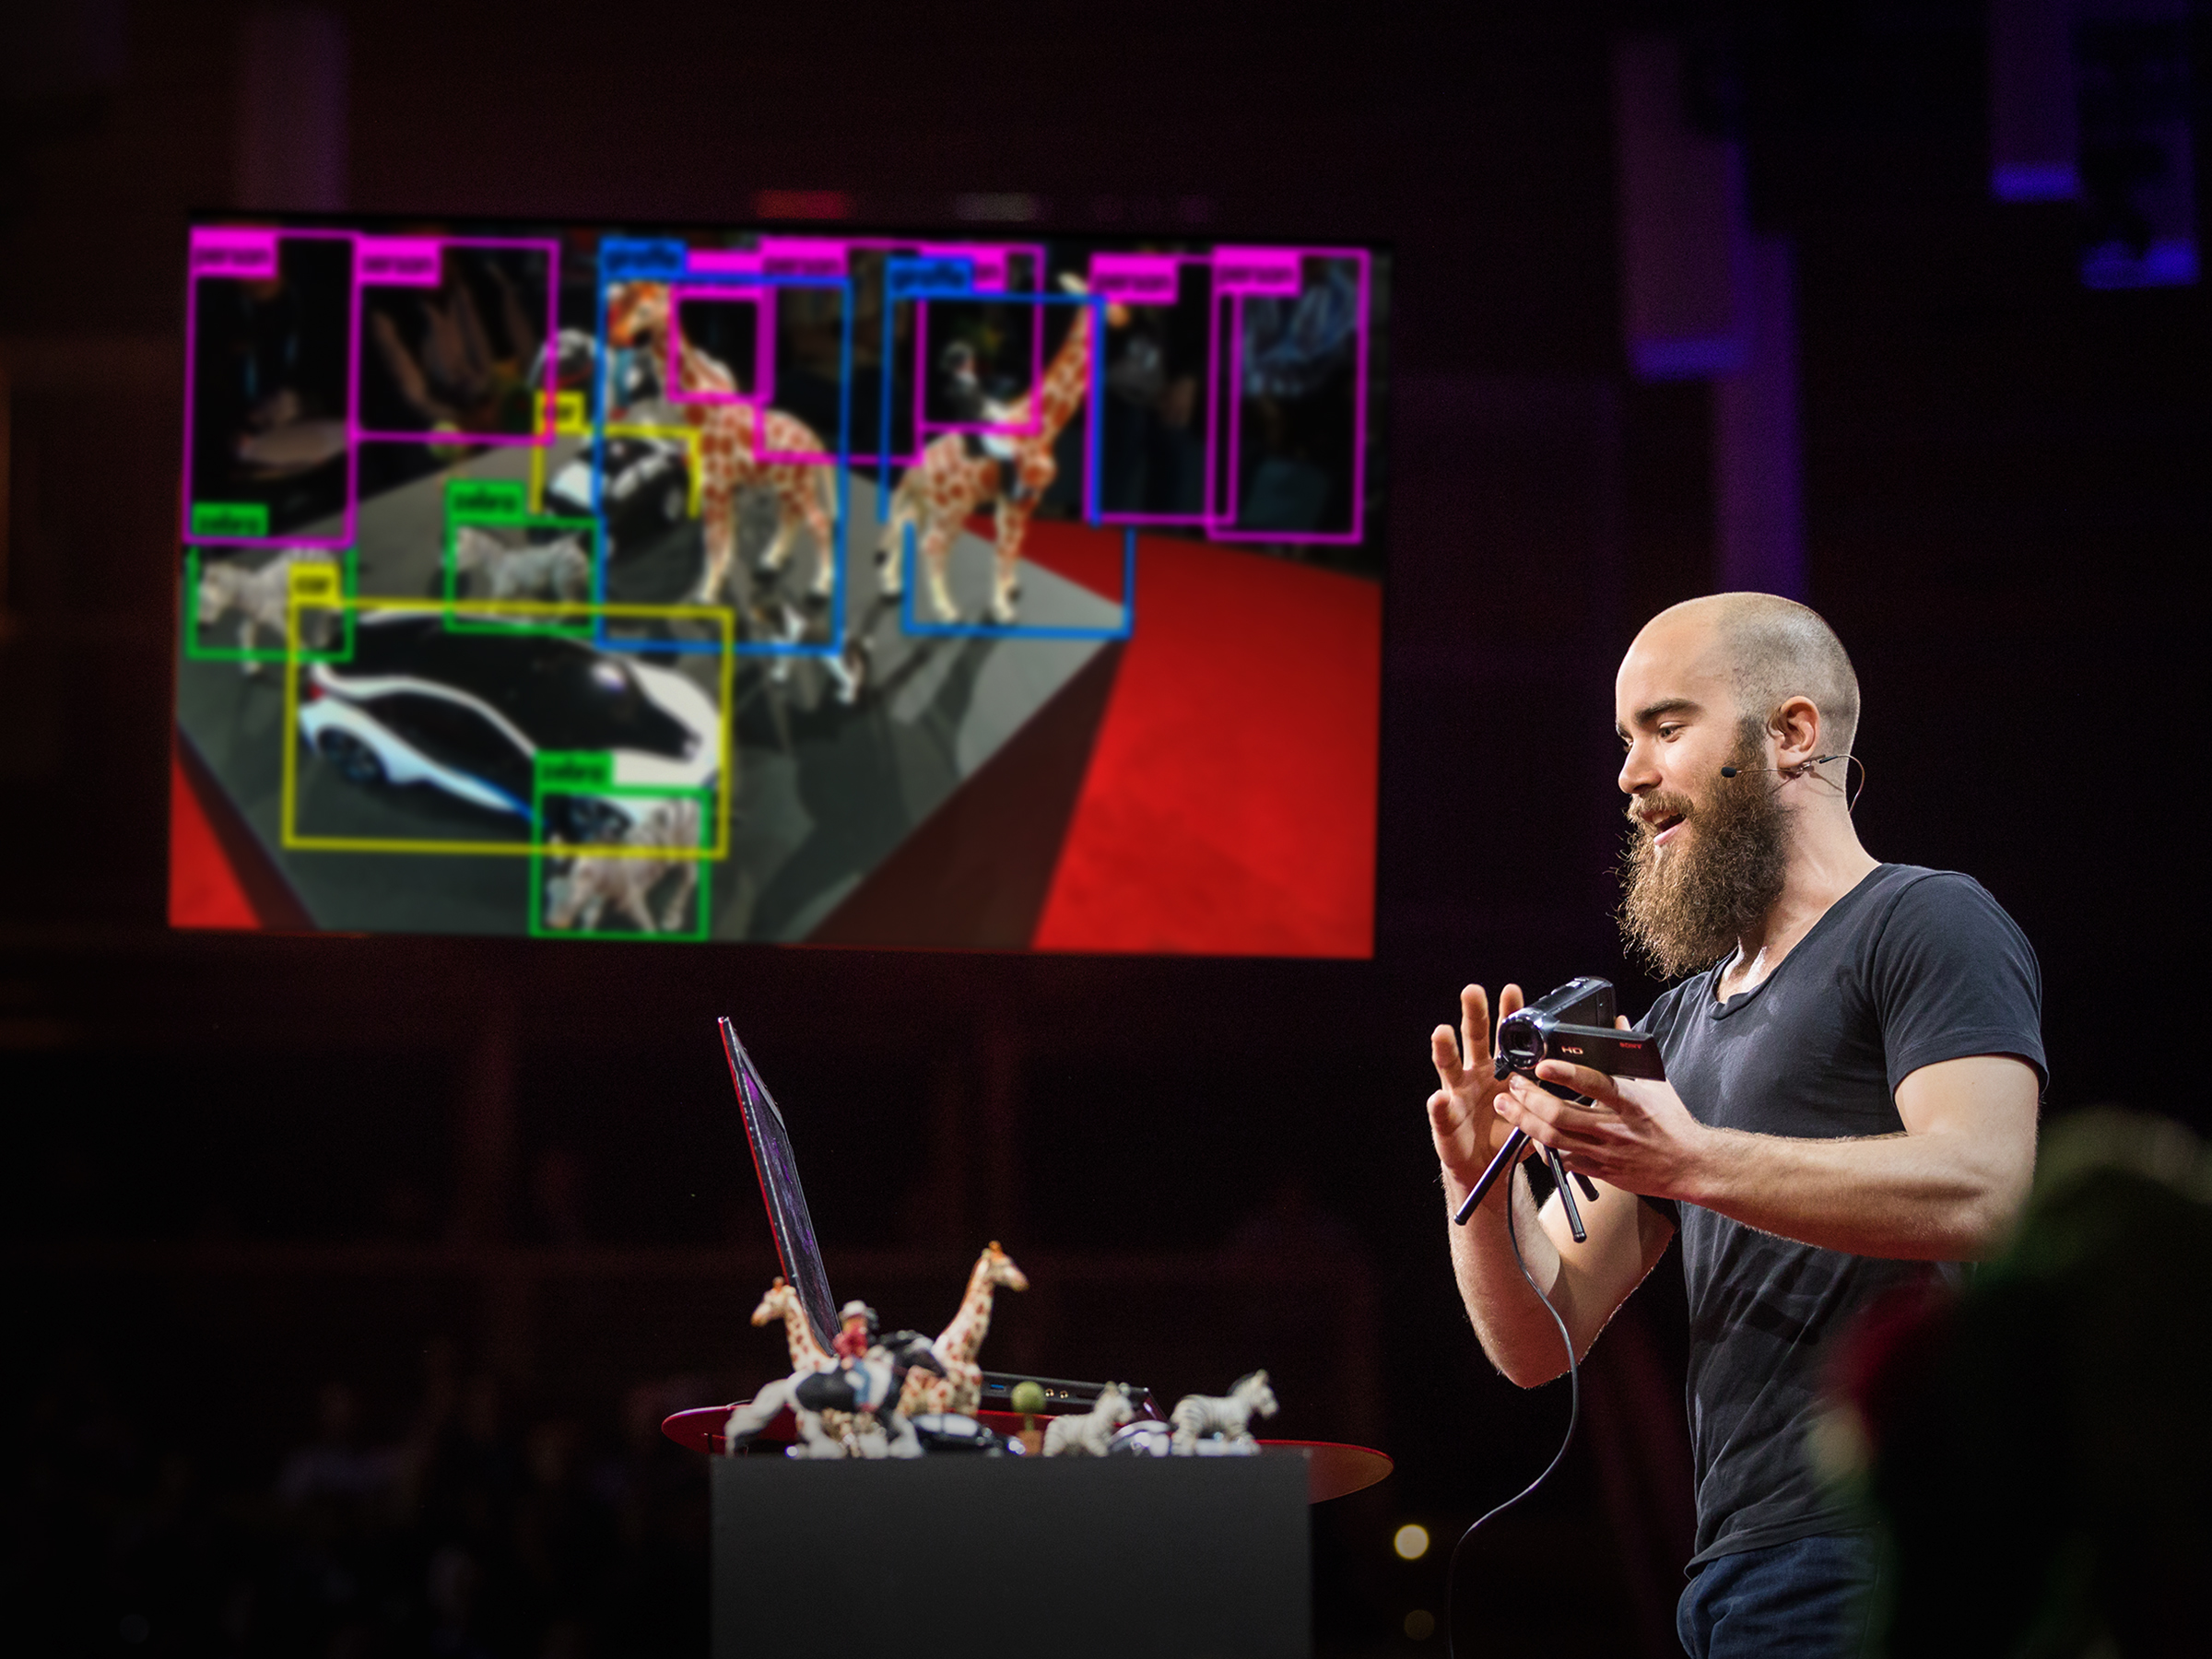
\includegraphics[width=0.8\textwidth]{files/capitoli/2-yolo/assets/joseph-redmon.jpeg}
    \caption{\label{fig:joseph-redmon}Joseph Redmon durante un TED Talk su YOLO nel 2017\cite{16}}
\end{figure}
\section{Evoluzione di YOLO}
YOLO ha subito un'evoluzione significativa nel corso degli anni, con ogni nuova versione che ha introdotto importanti miglioramenti in termini di precisione, velocità e capacità di generalizzazione.

\subsection{YOLOv1}
La prima versione di YOLO, proposta nel 2016\cite{14}, è composta da una singola rete neurale convoluzionale che processa l'intera immagine di input in un singolo passaggio. Nella rete troviamo le seguenti tipologie di layers:
\begin{itemize}
  \item \textbf{Convolutional Layers}: Applicano convoluzioni con filtri di diverse dimensioni per estrarre feature di alto livello dall'immagine di input. Questi strati sono responsabili della rilevazione dei pattern, come bordi, texture e forme complesse.
  \item \textbf{Max-Pooling Layers}: Ridimensionano le feature map riducendo la risoluzione spaziale, mantenendo le feature più importanti e riducendo la quantità di parametri e il costo computazionale. Max-pooling seleziona il valore massimo in ogni finestra del filtro, riducendo così l'informazione spaziale ma conservando le feature dominanti.
  \item \textbf{Fully Connected (FC) Layers}:  Connettono ogni unità di un layer a tutte le unità del layer successivo, combinando le feature estratte per produrre le predizioni finali. Questi strati sono utilizzati per la classificazione finale e la regressione delle bounding box.
\end{itemize}

L'architettura di YOLOv1 si ispira a GoogLeNet (rete nota per i suoi moduli inception che permettono di utilizzare filtri di diverse dimensioni in parallelo) e utilizza 24 convolutional layers per estrarre feature rilevanti a vari livelli di astrazione, alternati a max-pooling layers per ridurre la dimensione spaziale delle feature maps, mantenendo al contempo le informazioni più important. Successivamente, 2 FC layers combinano queste feature estratte per predire le bounding box e le probabilità di classe.


\begin{figure}[ht]
    \centering
    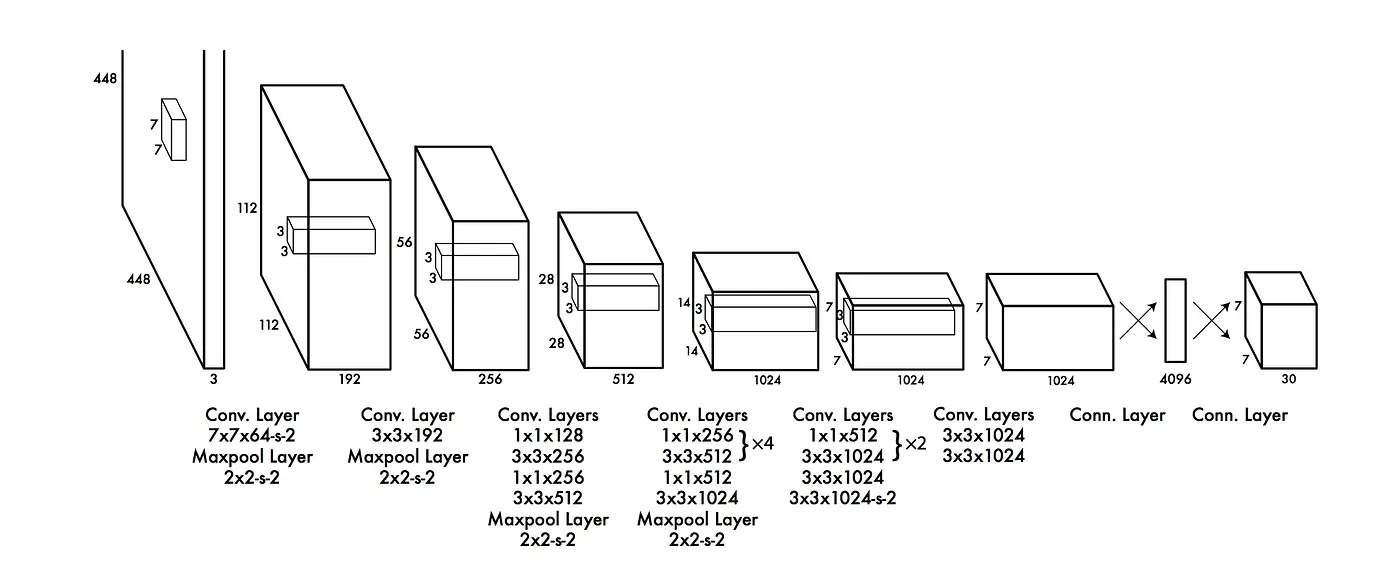
\includegraphics[width=1\textwidth]{files/capitoli/2-yolo/assets/yolov1-architecture.png}
    \caption{\label{fig:yolov1-architecture}Architettura di YOLOv1\cite{17}}
\end{figure}

L'output finale della rete è un tensore di dimensione
\[ S*S*(B*5 + C) \]
dove S è la dimensione della griglia, B è il numero di bounding box predette per cella, e C è il numero di classi. Questo tensore contiene tutte le predizioni delle bounding box, i punteggi di confidenza relativi a ciascuna predizione e le probabilità di classe per ogni oggetto rilevato.

\newpage

\subsection{YOLOv2}
YOLOv2, anche conosciuto come YOLO9000, è stato introdotto nel 2016\cite{18}; questa versione è stata progettata per essere più veloce e precisa, capace di rilevare una gamma più ampia di classi di oggetti.

Le caratteristiche principali includono:
\begin{itemize}
  \item \textbf{Backbone CNN Darknet-19}: YOLOv2 utilizza Darknet-19 come Backbone, una variante dell'architettura VGGNet, con strati di convoluzione progressiva e max-pooling.
  \item \textbf{Anchor Boxes}: introduce le Anchor Boxes, che sono bounding boxes predefinite con diverse proporzioni e scale., le quali permottono al modello di gestire meglio oggetti di varie dimensioni e proporzioni all'interno di un'immagine.
  \item \textbf{Batch Normalization}: l'introduzione della normalizzazione batch standardizza le attivazioni di ogni layer, riducendo il rischio di overfitting e accelerando la convergenza durante l'addestramento. Questo processo aiuta a mantenere l'output di ogni layer stabile e ben bilanciato, facilitando l'apprendimento di feature utili.
  \item \textbf{Strategia di Training Multi-Scale}: viene adottata una strategia di training multi-scala, che consiste nell'addestrare il modello su immagini di diverse scale e risoluzioni. Questa tecnica permette al modello di essere robusto e flessibile, adattandosi meglio a variazioni nelle dimensioni degli oggetti e migliorando la capacità di generalizzazione.
  \item \textbf{Nuova Loss Function}: introdotta una nuova loss function progettata specificamente per l'object detection, la quale è basata sugli errori quadratici tra le bounding box predette e quelle reali, e tiene conto anche delle probabilità di classe. La nuova loss function aiuta il modello a migliorare la precisione delle predizioni, penalizzando in modo appropriato le deviazioni tra le bounding box previste e quelle effettive, e ottimizzando la classificazione degli oggetti rilevati.
\end{itemize}

\begin{figure}[ht]
    \centering
    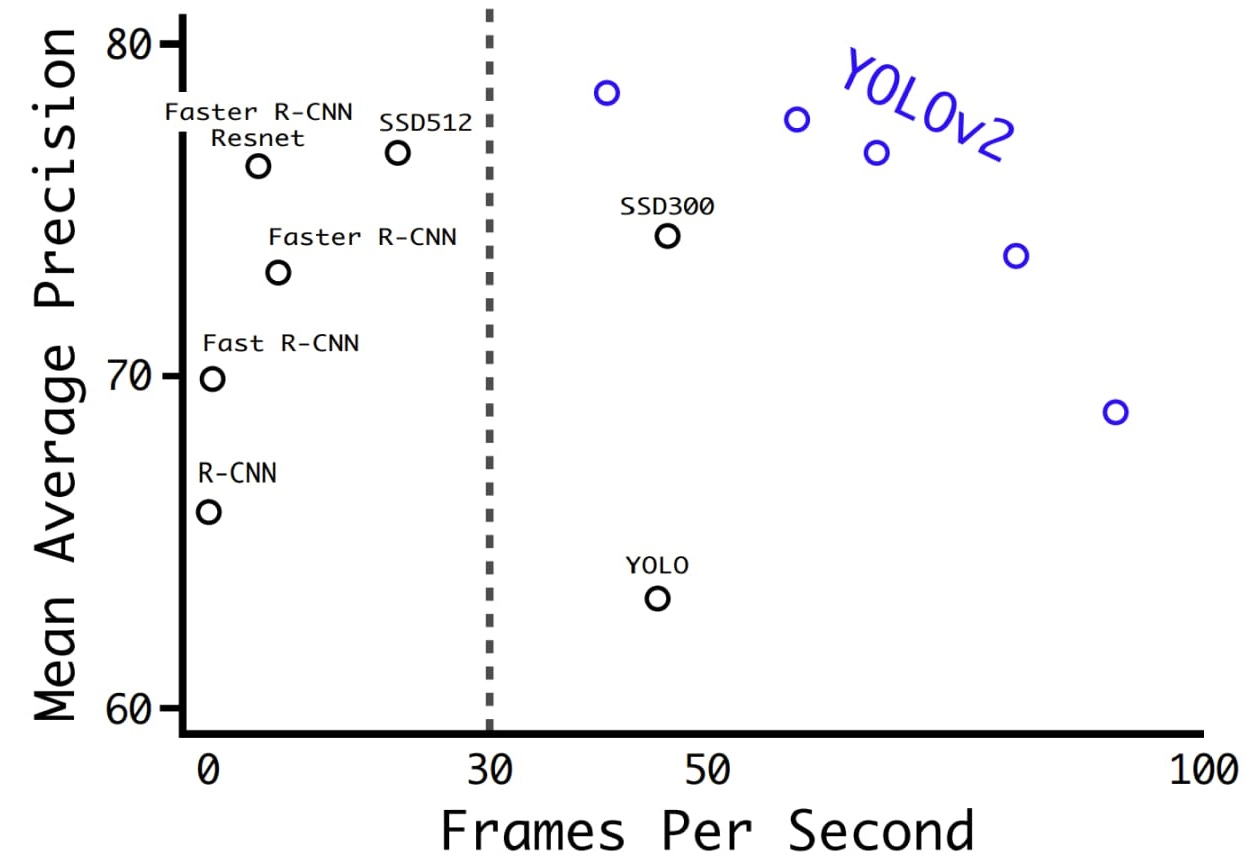
\includegraphics[width=0.7\textwidth]{files/capitoli/2-yolo/assets/yolov2-benchmark.jpeg}
    \caption{\label{fig:yolov2-benchmark}Confronto della mAP di YOLOv2 con quelle di altri modelli\cite{19}}
\end{figure}

\subsection{YOLOv3}
YOLOv3 è la terza versione dell'algoritmo YOLO, introdotta nel 2018\cite{20} con l'obiettivo di aumentare l'accuratezza e la velocità dell'algoritmo. Caratteristiche chiave di YOLOv3 sono:
\begin{itemize}
  \item \textbf{Architettura CNN Darknet-53}: Darknet-53 è una variante dell'architettura ResNet, progettata specificamente per le attività di object detection con 53 convolutional layers.
  \item \textbf{Anchor Boxes migliori}: Implementa anchor boxes scalate e con diversi aspect ratio per adattarsi meglio alle dimensioni e alle forme degli oggetti da rilevare.
  \item \textbf{Feature Pyramid Networks}: Introduce le FPN, una architettura CNN utilizzata per rilevare oggetti a diverse scale, migliorando le prestazioni di detection sugli oggetti di piccole dimensioni.
\end{itemize}

\vspace{1cm}

\begin{figure}[ht]
    \centering
    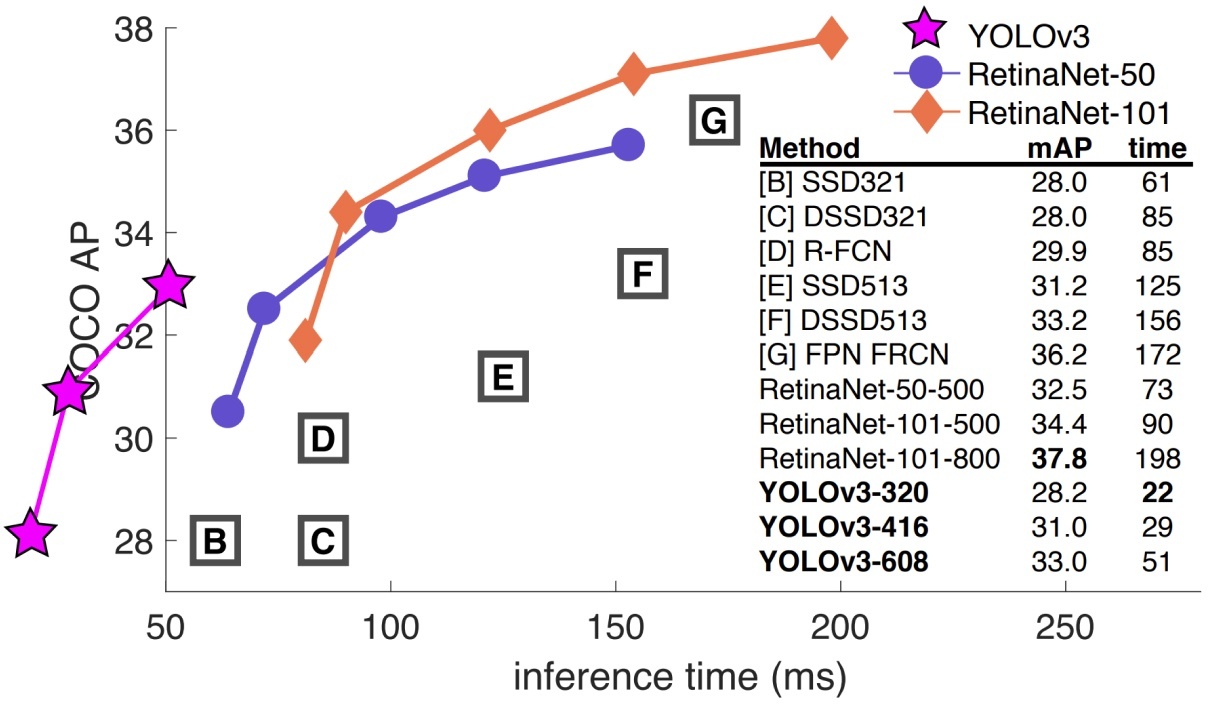
\includegraphics[width=0.8\textwidth]{files/capitoli/2-yolo/assets/yolov3-benchmark.jpeg}
    \caption{\label{fig:yolov3-benchmark}mAP ottenuta su dataset COCO con YOLOv3\cite{19}}
\end{figure}

\subsection{YOLOv4}

YOLOv4 viene rilasciata nel 2020 da Bochkovskiy\cite{21} e presenta le seguenti novità:
\begin{itemize}
  \item \textbf{Architettura CSPNet}: adotta una nuova architettura CNN chiamata CSPNet (Cross Stage Partial Network), una variante della ResNet progettata specificamente per task di object detection.
  \item \textbf{Anchor Box con k-means clustering}: introdotto un nuovo metodo di generazione per le anchor box che sfrutta un algoritmo di clustering per raggruppare le bounding box del ground truth in cluster, utilizzando i centroidi di questi cluster come anchor box; questo permette alle anchor box di essere più precise rispetto alle dimensioni e alla forma degli oggetti rilevati.
  \item \textbf{GHM Loss}: introdotta una variante della Focal Loss, progettata per migliorare le prestazioni del modello su dataset con distribuzione non uniforme delle classi.
  \item \textbf{Miglioramenti alle FPN}: revisione che migliora ulteriormente la capacità del modello di rilevare oggetti di piccole dimensioni, in modo da operare efficacemente su scale diverse all'interno delle immagini.
\end{itemize}

\begin{figure}[ht]
    \centering
    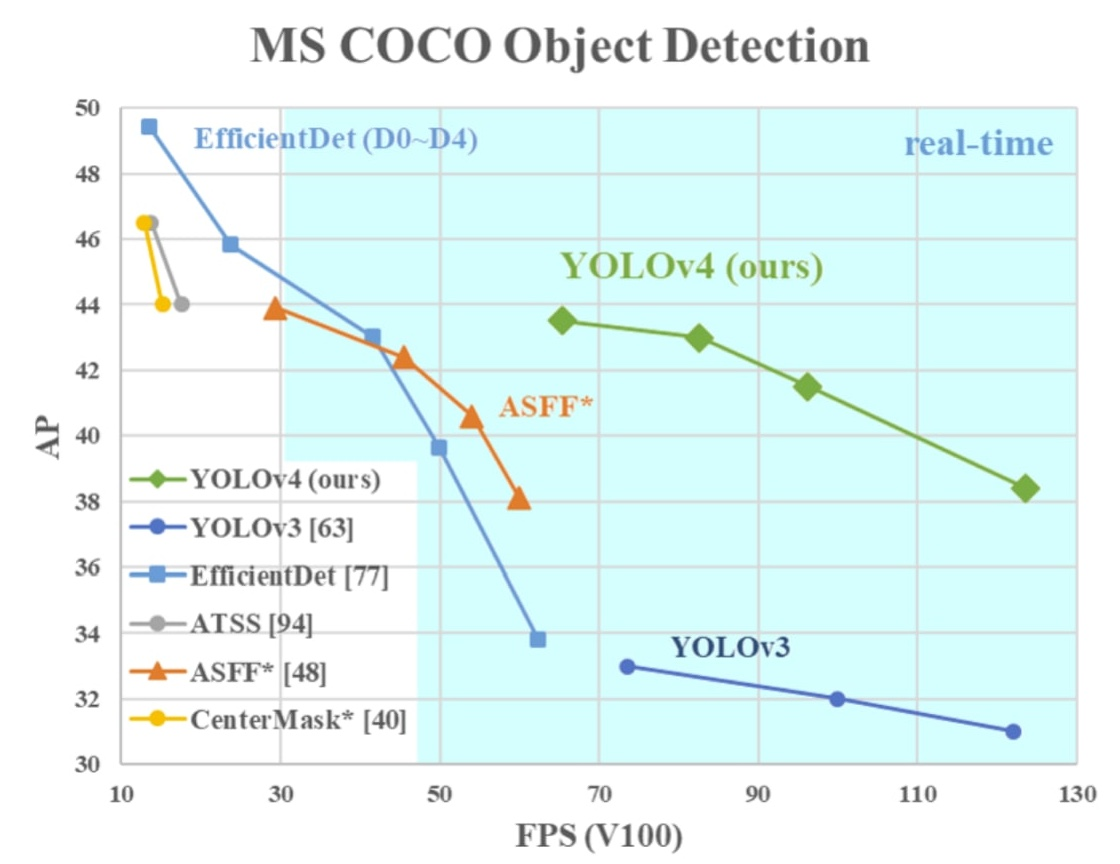
\includegraphics[width=0.8\textwidth]{files/capitoli/2-yolo/assets/yolov4-benchmark.jpeg}
    \caption{\label{fig:yolov4-benchmark}mAP di YOLOv4 confrontata con quelle di modelli precedenti\cite{19}}
\end{figure}

\newpage

\subsection{YOLOv5}
Introdotta nel 2020 dallo stesso team che ha sviluppato l'algoritmo YOLO originale, YOLOv5 è un progetto open-source mantenuto da Ultralytics\cite{22}. Introduce diverse nuove funzionalità e miglioramenti tra cui:
\begin{itemize}
  \item \textbf{Architettura EfficientDet}: utilizza una architettura più complessa chiamata EfficientDet, basata sull'architettura di rete EfficientNet, la quale consente a YOLOv5 di raggiungere una maggiore accuratezza e una migliore generalizzazione su un'ampia gamma di categorie di oggetti rispetto alle versioni precedenti.
  \item \textbf{Addestramento su Dataset Diversificato (D5)}: a differenza di YOLO, che è stato addestrato sul dataset PASCAL VOC composto da 20 categorie di oggetti, YOLOv5 è addestrato su un dataset più ampio e diversificato chiamato D5, che include un totale di 600 categorie di oggetti.
  \item \textbf{Spatial Pyramid Pooling (SPP)}: introduce un nuovo tipo di layer di pooling che riduce la risoluzione spaziale delle feature maps, il quale è particolarmente efficace nel migliorare le prestazioni di rilevamento sugli oggetti di piccole dimensioni, consentendo al modello di analizzare gli oggetti a diverse scale.
   \item \textbf{Loss Function CIoU}: introduce una nuova loss function chiamata "CIoU loss", variante della loss function IoU (Intersection over Union). La CIoU loss è specificamente progettata per migliorare le prestazioni del modello su dataset sbilanciati, contribuendo a migliorare l'accuratezza e la stabilità durante l'addestramento.
\end{itemize}

\newpage

\begin{figure}[ht]
    \centering
    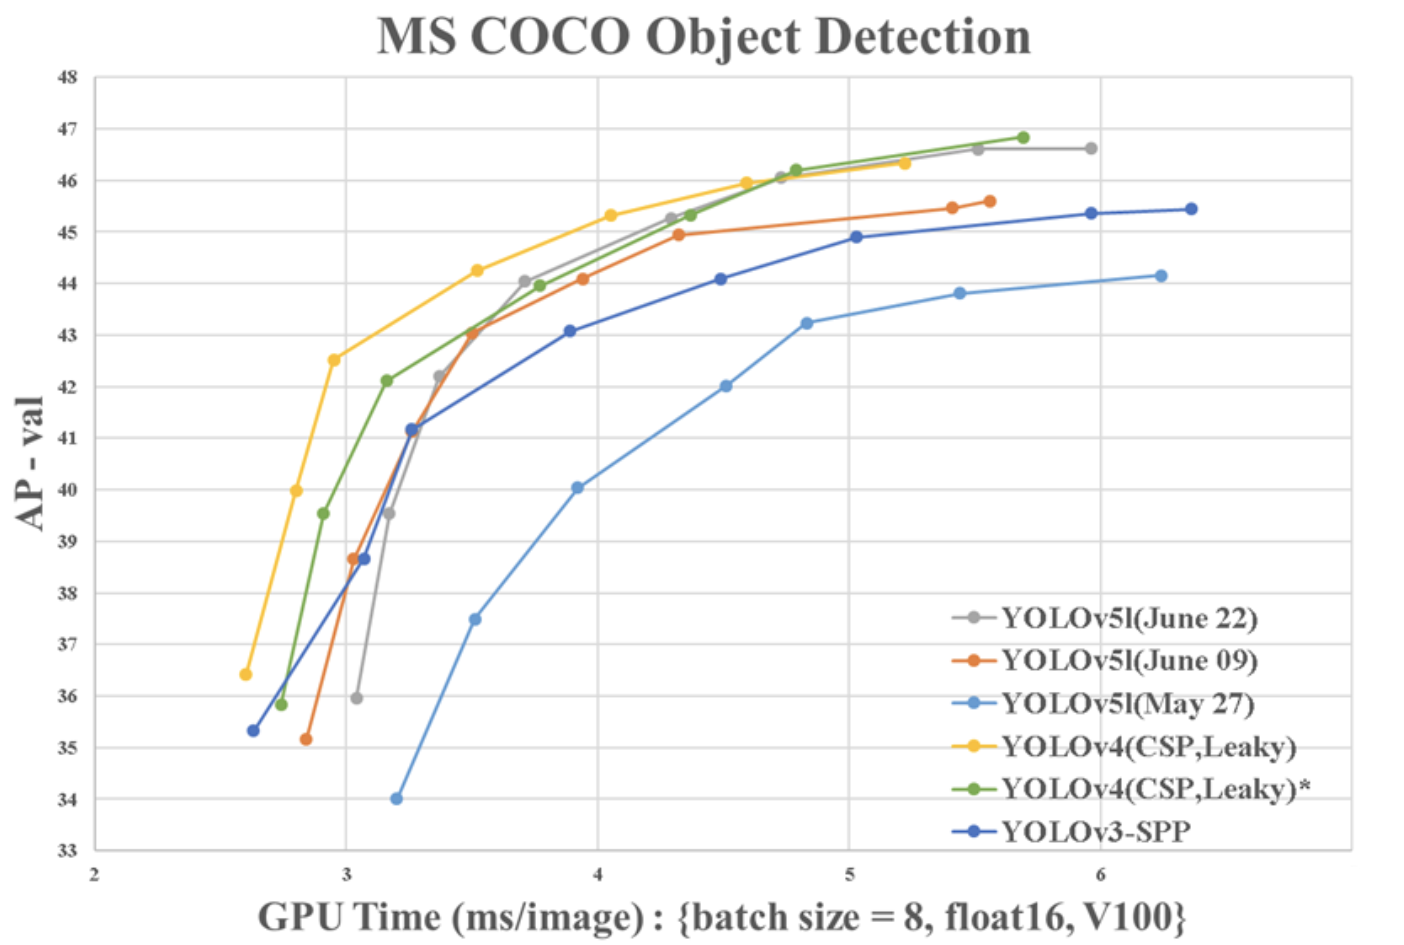
\includegraphics[width=0.9\textwidth]{files/capitoli/2-yolo/assets/yolov5-benchmark.png}
    \caption{\label{fig:yolov5-benchmark}mAP di YOLOv5 confrontata con quelle di modelli precedenti\cite{23}}
\end{figure}

\subsection{YOLOv6}
Proposta nel 2020 da Li et al.\cite{24}, va a migliorare le precedenti versioni introducento una nuova architettura CNN chiamata \textbf{EfficientNet-L2}, una variante dell'architettura EfficientNet che migliora l'efficienza computazionale del modello riducendo il numero di parametri, pur mantenendo elevate prestazioni su vari benchmark di object detection.

\newpage

\subsection{YOLOv7}
La settima versione di YOLO, rilasciata nel 2022 da Chien-Yao Wang, Alexey Bochkovskiy e Hong-Yuan Mark Liao\cite{25}, introduce diverse migliorie significative:
\begin{itemize}
  \item \textbf{Anchor boxes migliorate}: YOLOv7 aumenta a 9 il numero di anchor boxes, il quale permette al modello di rilevare una gamma più ampia di forme e dimensioni degli oggetti rispetto alle versioni precedenti, riducendo così il numero di falsi positivi.
  \item \textbf{Focal Loss}: introdotta una nuova loss function chiamata "focal loss", la quale riduce il peso della loss per esempi ben classificati e si concentran sugli esempi difficili, ovvero gli oggetti difficili da rilevare.
  \item \textbf{Risoluzione più alta e velocità migliorata}: YOLOv7 processa le immagini ad una risoluzione superiore rispetto alle versioni precedenti, ottenendo una precisione complessiva maggiore, ed ad una velocità maggiore, rendendolo adatto per applicazioni sensibili in tempo reale dove velocità di elaborazione più elevate sono cruciali.
\end{itemize}

\newpage
\section{Modelli utilizzati}
I tre modelli selezionati per la sperimentazione di questa tesi (YOLOv8, YOLO-World e RT-DETR) rappresentano l'avanguardia nell'ambito dell'Object Detection. Ognuno di essi presenta caratteristiche uniche che li rendono adatti a diversi scenari applicativi, rappresentando un ulteriore sviluppo rispetto alle precedenti iterazioni dei modelli YOLO.

\subsection{YOLOv8}
YOLOv8 rappresenta l'ultima evoluzione della famiglia YOLO, sviluppata da Ultralytics e rilasciata nel 2023\cite{26}. Questa versione introduce una serie di miglioramenti significativi rispetto alle precedenti, rendendolo uno degli algoritmi di rilevamento degli oggetti più avanzati e performanti disponibili oggi.

\subsubsection{Miglioramenti introdotti}
YOLOv8 introduce le seguenti migliorie: 
\begin{itemize}
  \item \textbf{Architettura Backbone}: YOLOv8 utilizza un'architettura backbone più avanzata che combina convolutional layers ottimizzati con tecniche di normalizzazione e attivazione migliorate, progettata per massimizzare l'estrazione delle feature mantenendo un alto livello di efficienza computazionale.
  \item \textbf{Residual Blocks e Dense Connections}: l'introduzione di residual blocks (simili a quelli di ResNet) e dense connections (ispirate a DenseNet) contribuisce a una migliore propagazione del gradiente durante l'addestramento. Vengono ridotti problemi come il vanishing gradient e migliorata la capacità della rete di apprendere rappresentazioni complesse, permettendo alla rete di addestrarsi.
  \item \textbf{GIoU Loss}: la loss function è stata migliorata con l'introduzione della Generalized Intersection over Union (GIoU) loss, la quale tiene conto non solo della sovrapposizione tra le bounding box previste e quelle reali, ma anche della distanza tra di esse.
  \item \textbf{Miglioramenti nelle FPN}: le feature pyramid networks sono state potenziate per fornire una migliore rappresentazione multi-scala delle feature dell'immagine, fattore che aiuta il modello a rilevare oggetti di diverse dimensioni, specialmente quelli piccoli.
  \item \textbf{Inferenza Accelerata}: grazie a ottimizzazioni specifiche nell'architettura e nell'implementazione del codice, YOLOv8 è in grado di eseguire l'inferenza a velocità superiori rispetto ai suoi predecessori.
  \item \textbf{Efficienza Computazionale}: la struttura generala è stata ottimizzata per essere eseguita su dispositivi con risorse limitate, come i dispositivi edge e embedded. 
  %Ciò rende YOLOv8 una scelta eccellente per applicazioni che devono girare su hardware a bassa potenza, come droni, telecamere di sicurezza e altri dispositivi IoT.
\end{itemize}

\begin{figure}[ht]
    \centering
    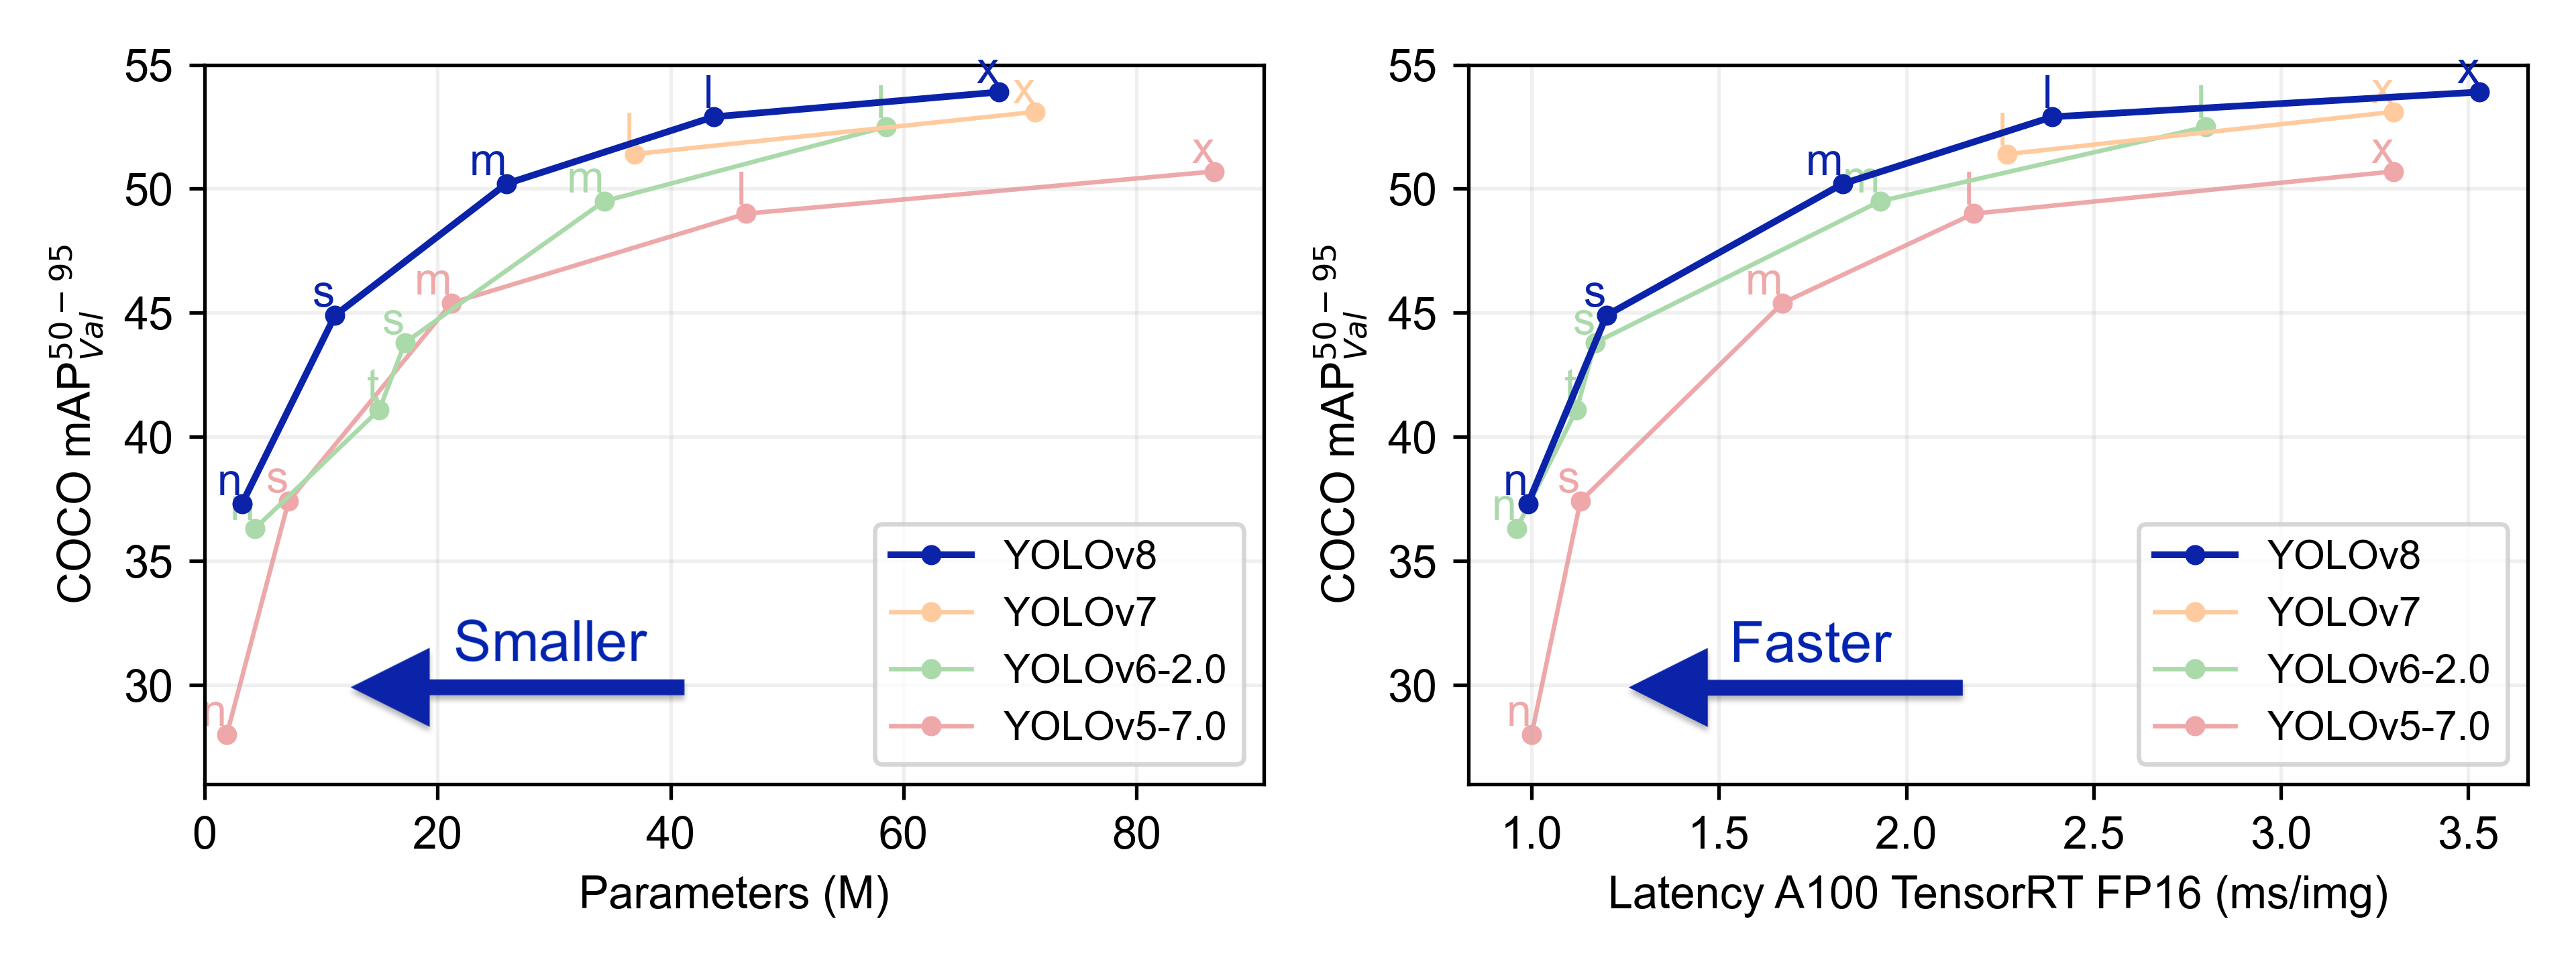
\includegraphics[width=0.95\textwidth]{files/capitoli/2-yolo/assets/yolov8-benchmark.png}
    \caption{\label{fig:yolov8-benchmark}mAP ottenuta da YOLOv8 su dataset COCO confrontata con quelle delle precedenti versioni\cite{27}}
\end{figure}

\newpage

\subsubsection{Architettura}
L'architettura di YOLOv8 si suddivide in 3 blocchi principali:
\begin{itemize}
  \item \textbf{Backbone}: chiamato anche Feature Extractor, è responsabile dell'estrazione delle feature significative dall'input. Nei suoi strati iniziali, rileva schemi semplici come bordi e texture, e man mano che si avanza, il backbone rileva feature a più scale, ottenendo rappresentazioni a diversi livelli di astrazione.
  \item \textbf{Neck}: funge da ponte tra il Backbone e il blocco successivo (Head). Esso costruisce piramidi di feature aggregando le feature maps ottenute dal backbone ed eseguendo la concatenazione o fusione di feature a diverse scale per garantire che la rete possa rilevare oggetti di diverse dimensioni. Inoltre, integra informazioni contestuali per migliorare l'accuratezza del rilevamento e riduce la risoluzione spaziale e la dimensionalità delle risorse per facilitare il calcolo, aumentando la velocità.
  \item \textbf{Head}: è la parte finale dell'architettura e si occupa di generare gli output della rete. Genera le bounding boxes associate ai possibili oggetti nell'immagine, assegna punteggi di confidenza a ciascuna bounding box per indicare la probabilità della presenza di un oggetto, e classifica gli oggetti nelle bounding boxes in base alle loro categorie.
\end{itemize}

\newpage

\begin{figure}[ht]
    \centering
    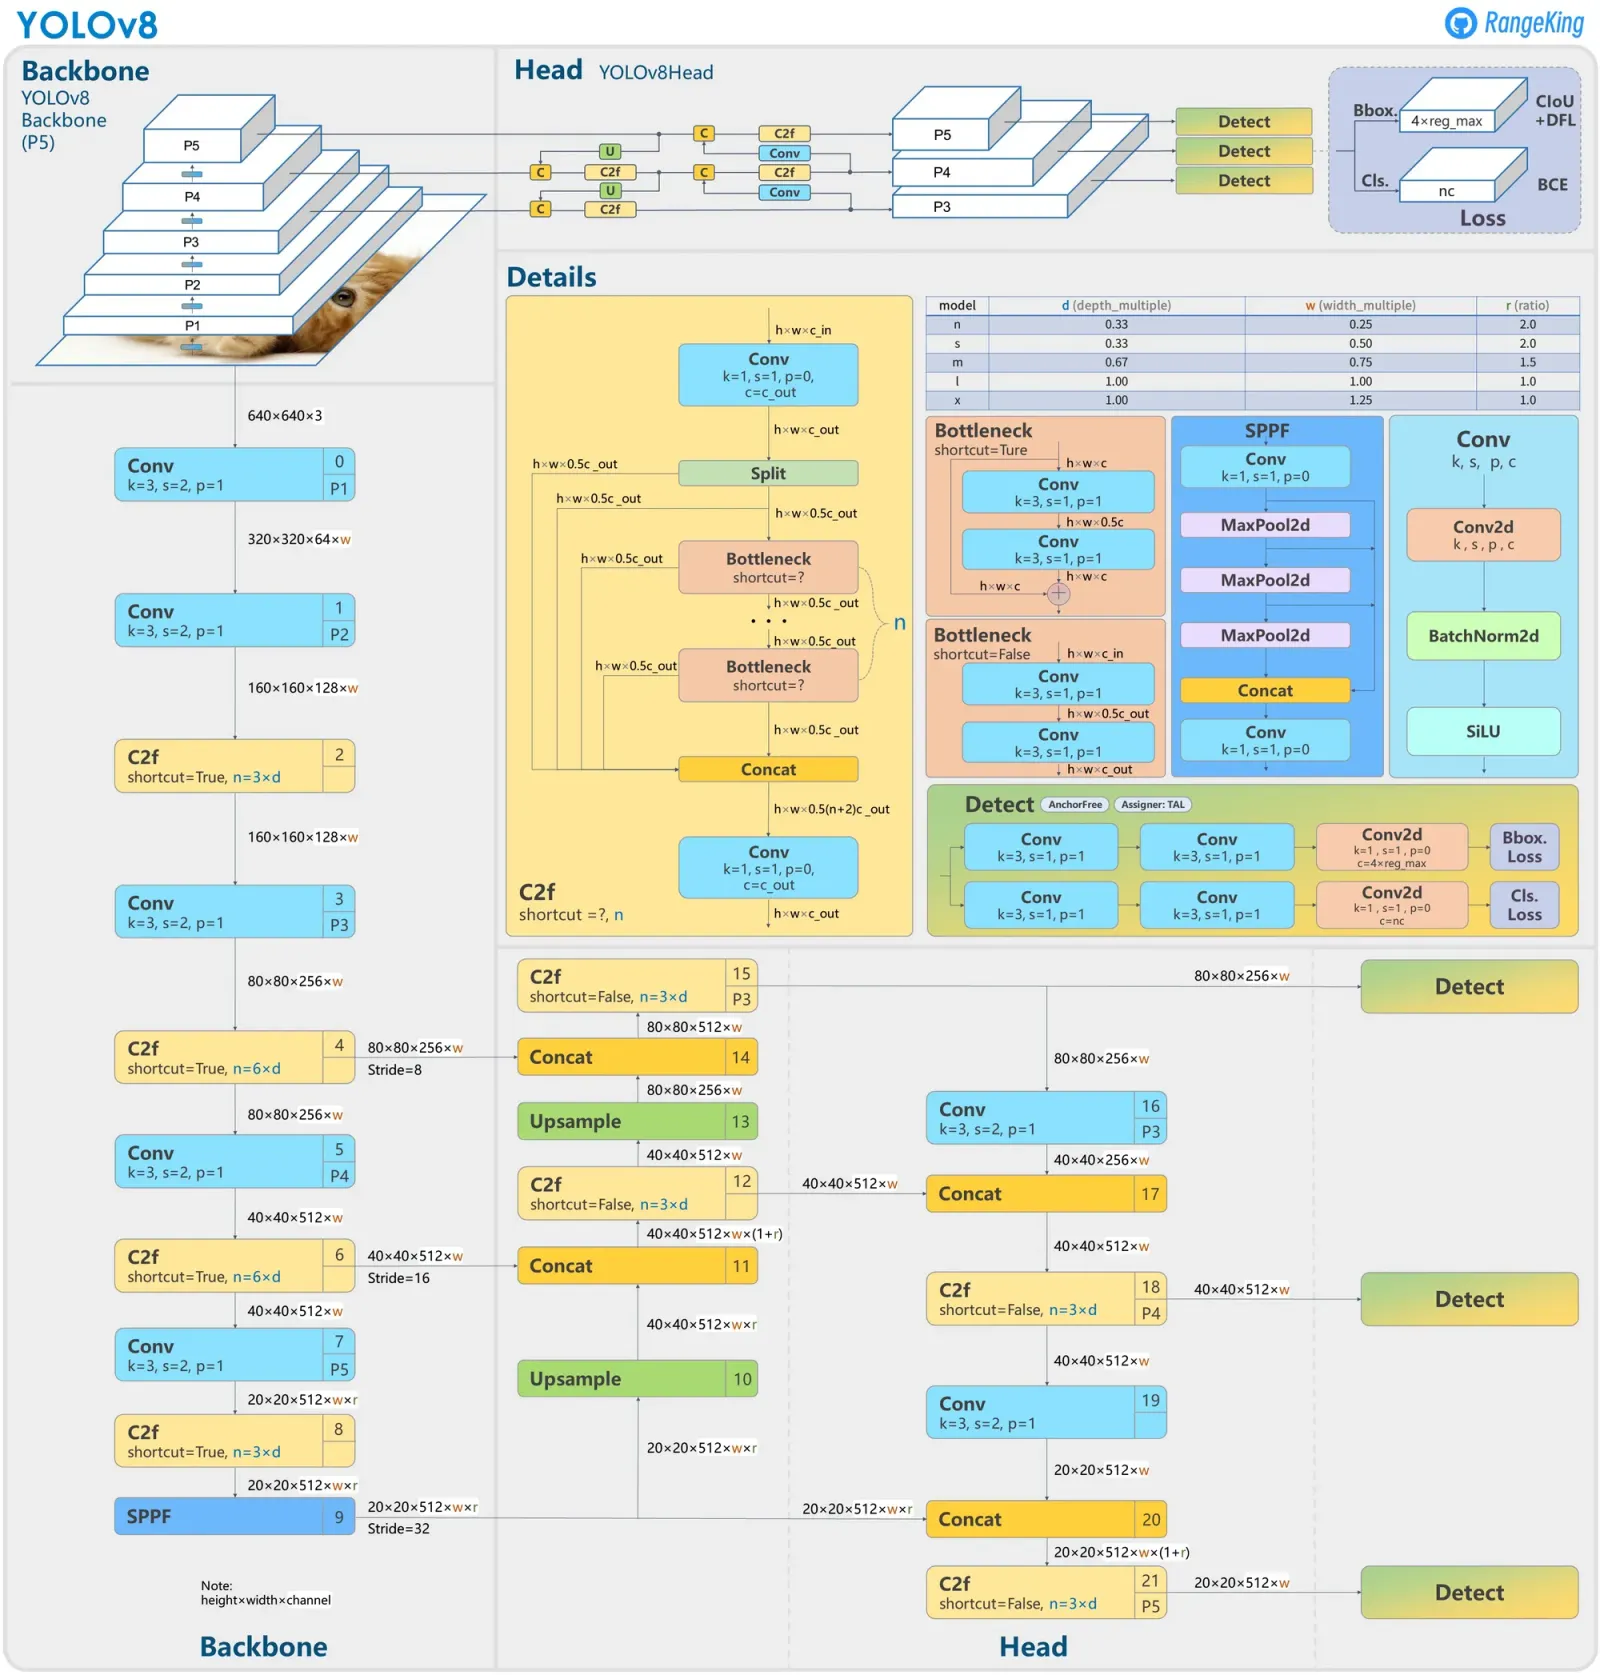
\includegraphics[width=1\textwidth]{files/capitoli/2-yolo/assets/yolov8-architecture.png}
    \caption{\label{fig:yolov8-architecture}Architettura di YOLOv8\cite{28}}
\end{figure}

\newpage

\subsection{YOLO-World}
YOLO-World è una recente evoluzione della famiglia di algoritmi YOLO\cite{29}, rivoluzionaria nella open-vocabulary object detection, che combina efficacemente l'efficienza di YOLOv8 con la potenza della modellazione vision-language ed un massiccio pre-training.

\subsubsection{Open-Vocabulary Object Detection}
L'object detection open-vocabulary (OVD) si propone di rilevare qualsiasi oggetto descritto tramite linguaggio naturale, anche se non è stato "visto" durante l'addestramento, superando così le limitazioni dei detector tradizionali che si concentrano su categorie di oggetti fissate.

YOLO-World in particolare consente di specificare dinamicamente le classi tramite prompt personalizzati, permettendo così agli utenti di adattare il modello alle proprie esigenze  senza doverlo addestrare nuovamente. Questa caratteristica è particolarmente utile per adattare il modello a nuovi domini o compiti specifici che non erano originariamente parte dei dati di addestramento. Impostando prompt personalizzati, gli utenti possono guidare il focus del modello verso gli oggetti di interesse, migliorando l'accuratezza dei risultati di detection.

\vspace{1cm}

\begin{figure}[ht]
    \centering
    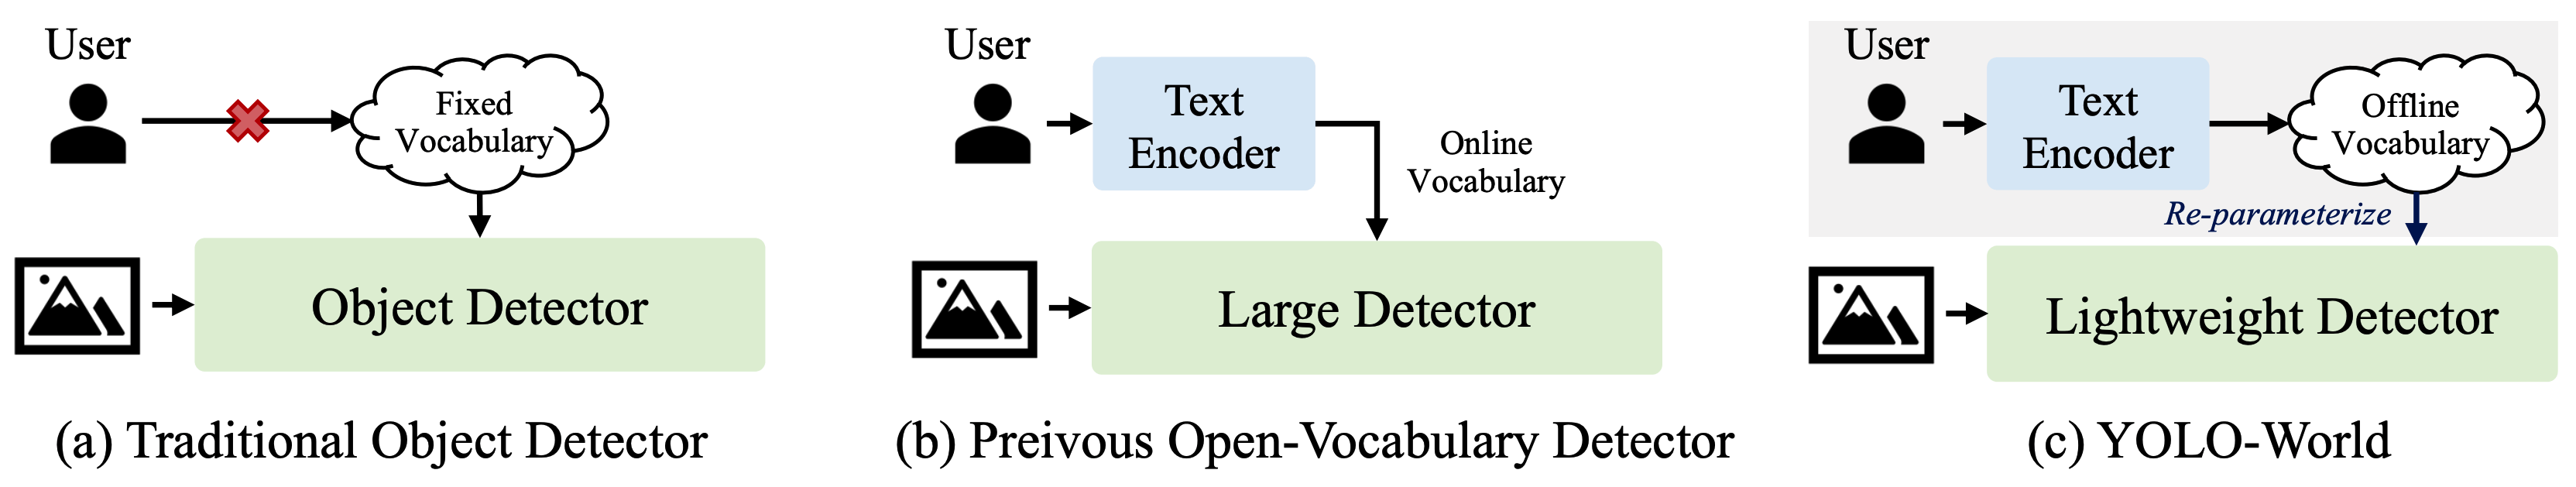
\includegraphics[width=1\textwidth]{files/capitoli/2-yolo/assets/yoloworld-ovd.png}
    \caption{\label{fig:yoloworld-ovd}Open-Vocabulary Object Detection di YOLO-World\cite{30}}
\end{figure}

\subsubsection{Innovazioni introdotte}
YOLO-World introduce le seguenti innovazioni:
\begin{itemize}
  \item \textbf{Paradigma Prompt-Then-Detect}: precomputando vocabolari offline basati su prompt definiti dall'utente, YOLO-World evita la necessità di codifica del testo in tempo reale, migliorando la velocità di inferenza e semplificando la personalizzazione.
  \item \textbf{Vision-Language Grounding}: la capacità del modello di comprendere e correlare informazioni visive con descrizioni in linguaggio naturale porta a rilevazioni più precise e consapevoli del contesto.
  \item \textbf{Ridotta Complessità del Modello}: la sua architettura evita le pesanti componenti basati su Transformer presenti nei modelli OVD precedenti, promuovendo l'accessibilità.
  \item \textbf{Etica Open-Source}: rilasciato sotto la GPL (General Public License), favorisce la collaborazione, accelera l'innovazione e garantisce che la tecnologia rimanga accessibile alla comunità più ampia.
\end{itemize}

\subsubsection{Architettura}
Le componenti principali dell'architettura di YOLO-World:
\begin{itemize}
  \item \textbf{YOLOv8 Backbone}: si occupa dell'estrazione delle feature, fornendo dettagliate rappresentazioni multi-scala delle immagini in input.
  \item \textbf{Text Encoder}: un encoder basato su Transformer (che sfrutta i progressi ottenuti da CLIP di OpenAI) utile a trasformare efficientemente i prompt in linguaggio naturale in embedding testuali informativi.
  \item \textbf{RepVL-PAN}: il Re-parameterizable Vision-Language Path Aggregation Network combina in modo efficace le feature visive e gli embedding testuali. Questa sinergia è ottenuta tramite:
  \begin{itemize}
    \item \textbf{Text-guided Cross Stage Partial Layer (T-CSPLayer)}, il quale potenzia le feature dell'immagine tramite le indicazioni degli embedding testuali, dirigendo l'attenzione del modello verso aree rilevanti. Questo avviene tramite il Max Sigmoid Attention Block, che calcola i pesi di attenzione basati sull'interazione tra le indicazioni testuali e le caratteristiche spaziali dell'immagine.
    \item \textbf{Image-Pooling Attention}, che "raffina" gli embedding testuali incorporando il contesto visivo globale e così migliorando la comprensione complessiva.
  \end{itemize}
\end{itemize}

\vspace{1cm}

\begin{figure}[ht]
    \centering
    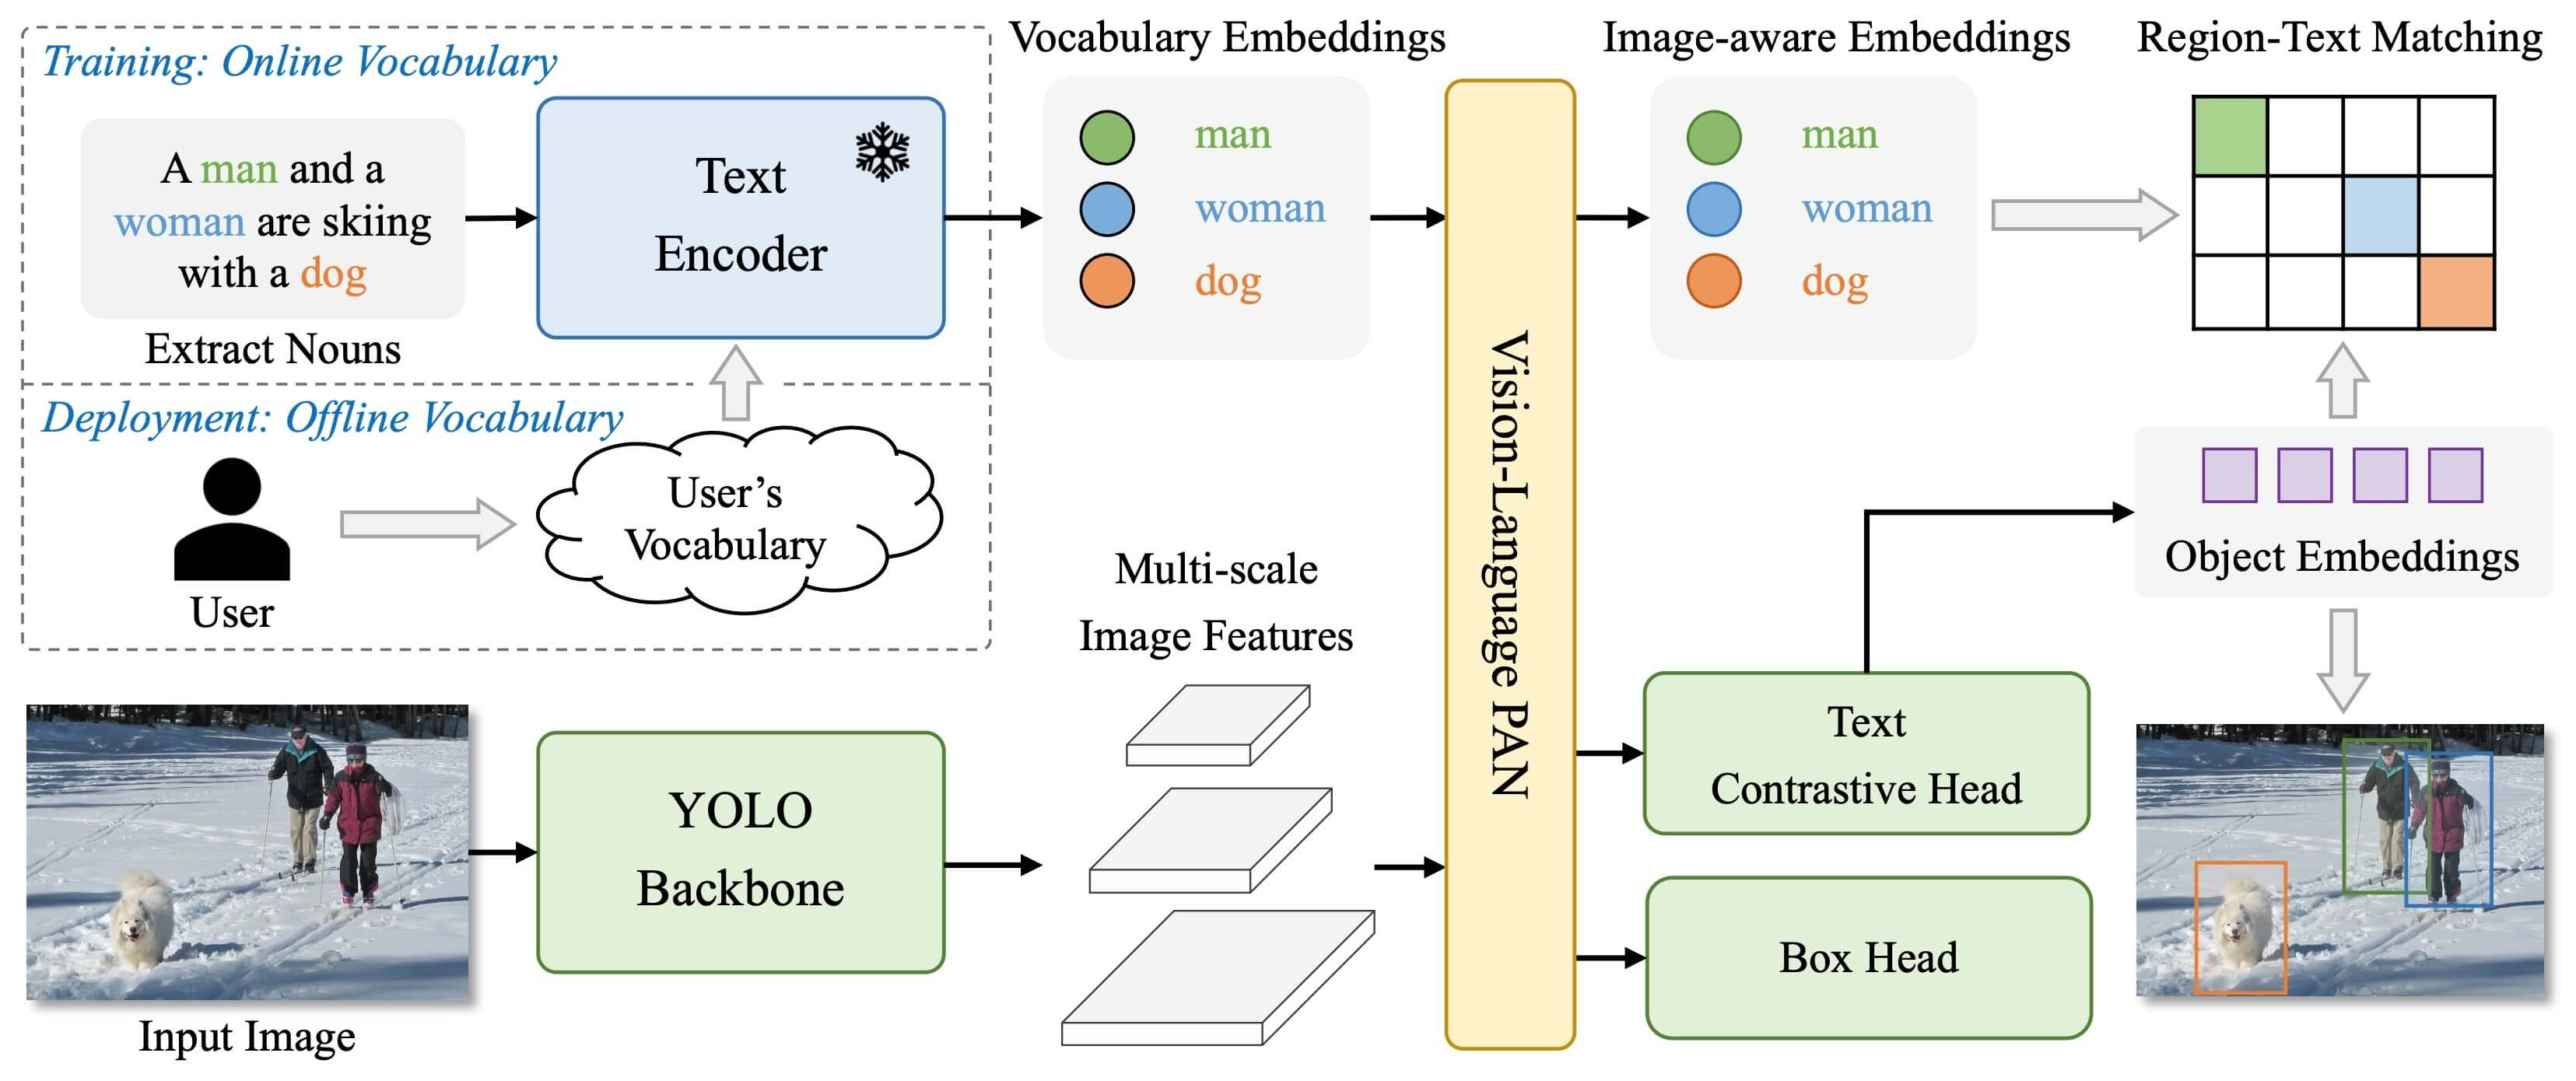
\includegraphics[width=1\textwidth]{files/capitoli/2-yolo/assets/yoloworld-architecture.jpeg}
    \caption{\label{fig:yoloworld-architecture}Architettura di YOLO-World\cite{30}}
\end{figure}

\newpage

\subsection{RT-DETR}
RT-DETR, o Real-Time DETR, è un'evoluzione del modello DETR (DEtection TRansformer) sviluppato da Baidu\cite{31}, che mira a migliorare le prestazioni di object detection in tempo reale.

\subsubsection{Caratteristiche principali}
Le principali caratteristiche del modello RT-DETR sono:
\begin{itemize}
  \item \textbf{Efficient Hybrid Encoder}: incorpora un encoder che sfrutta i Vision Transformers (ViT) per gestire efficientemente le feature multiscala, permettendo così al RT-DETR di acquisire una comprensione globale delle immagini, migliorando la capacità di rilevamento degli oggetti senza dipendere esclusivamente da filtri locali come nelle CNN.
  \item \textbf{Selezione delle Query consapevole dell'IoU}: migliora l'inizializzazione delle query degli oggetti attraverso una selezione consapevole dell'indice di sovrapposizione (IoU), permettendo al modello di concentrarsi sugli oggetti più pertinenti della scena e migliorando l'accuratezza della detection.
  \item \textbf{Velocità di Inferenza Adattabile}: offre flessibilità nella regolazione della velocità di inferenza utilizzando diversi strati del decoder senza necessità di riaddestramento
\end{itemize}

\subsubsection{Architettura}
L'architettura di RT-DETR consiste sempre in 3 componenti principali:
\begin{itemize}
  \item \textbf{Backbone}: utilizza un approccio innovativo il quale non si limita alla selezione delle feature map finali del backbone, bensì utilizza feature provenienti da tre diversi livelli diversi di quest'ultimo. Gli stadi S3, S4 e S5 del backbone vengono impiegati come input per l'encoder, fungendo così da estrattore di caratteristiche multiscala per il modello.
  \item \textbf{Efficient Hybrid Encoder}: trasforma le feature in una sequenza di feature dell'immagine, utilizzando due altri moduli:
  \begin{itemize}
    \item \textbf{AIFI (Attention based Intra Scale Feature Interaction)}, il quale si occupa esclusivamente della feature map S5 per estrarre interpretazioni semantiche più elaborate, aumentando l'accuratezza complessiva.
    \item \textbf{CCFM (CNN based Cross-scale Feature-fusion Module)}, che estrapola interpretazioni semantiche sia da S4 che da S5, ed incorpora un Fusion Block che fonde le caratteristiche di due blocchi adiacenti in una nuova feature.
  \end{itemize}
  \item \textbf{IoU Aware Query Selection e Transformer Decorder}: il primo è il modulo adibito alla selezione delle feature in base all'indice di sovrapposizione, le quali serviranno da input per il decoder, responsabile della generazione delle bounding box e dei punteggi di confidenza.
\end{itemize}

\begin{figure}[ht]
    \centering
    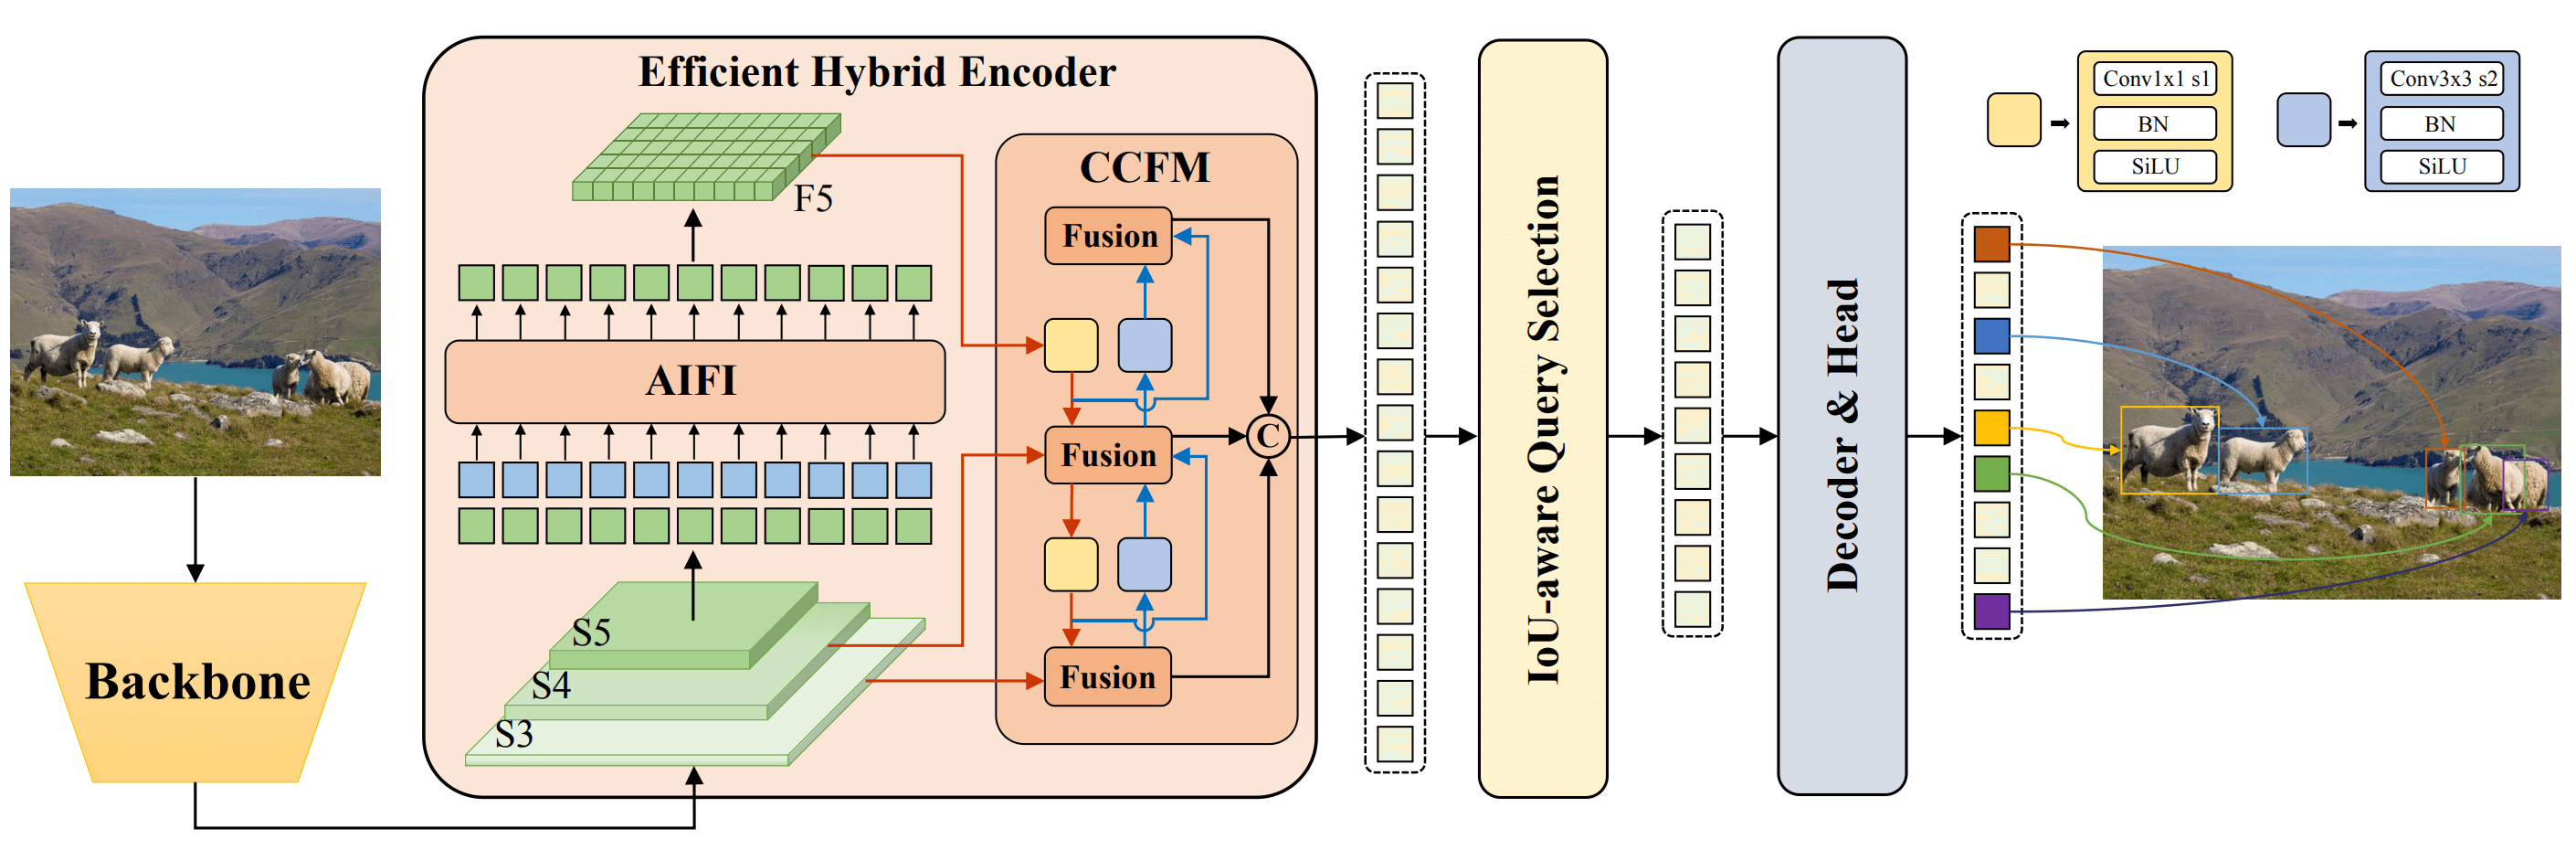
\includegraphics[width=1\textwidth]{files/capitoli/2-yolo/assets/rtdetr-architecture.png}
    \caption{\label{fig:rtdetr-architecture}Architettura di RT-DETR\cite{32}}
\end{figure}



\chapter{Data Augmentation}\label{ch:data-augmentation}

\section{Introduzione alla Data Augmentation}

\subsection{Definizione}
La data augmentation è una tecnica utilizzata nel campo del machine learning per incrementare la quantità e la varietà dei dati di addestramento a disposizione. 

\begin{figure}[ht]
    \centering
    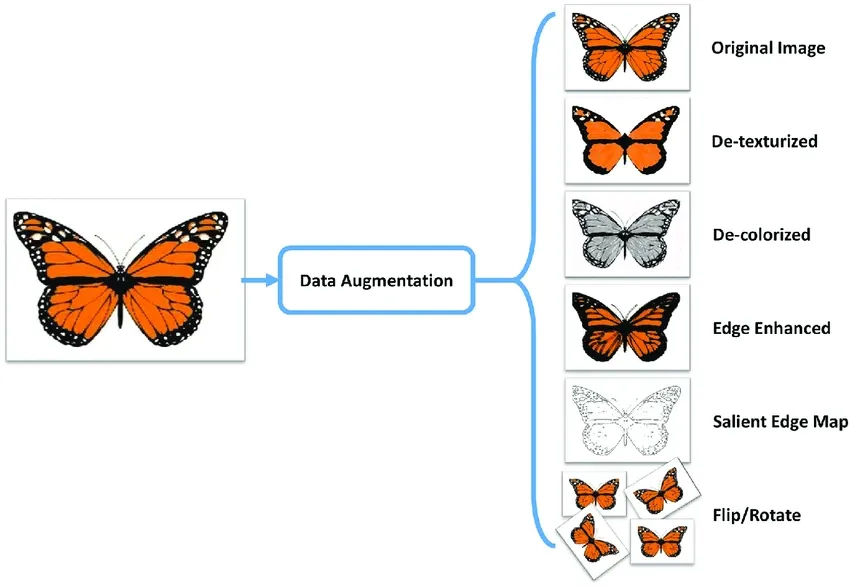
\includegraphics[width=0.7\textwidth]{files/capitoli/3-data-augmentation/assets/augmentation-example.png}
    \caption{\label{fig:augmentation-example}Esempi di Augementation su un'immagine\cite{33}}
\end{figure}

\newpage

Questa tecnica consiste nel generare nuovi dati a partire da quelli esistenti, applicando una serie di trasformazioni come rotazioni, traslazioni, modifiche di colore, aggiunta di rumore, e molte altre. Si può quindi definire come un insieme di operazioni che modificano i dati originali in modo da creare nuove versioni, pur mantenendo inalterata l'informazione essenziale contenuta nei dati stessi.

\subsection{Scopo}
L'obiettivo principale della data augmentation è quello di migliorare la generalizzazione dei modelli di machine learning, ovvero la capacità del modello di performare bene su dati mai visti prima. Questo viene ottenuto in vari modi:
\begin{itemize}
  \item \textbf{Aumento della Varietà dei Dati}: aggiungendo varianti dei dati esistenti, si espande il dataset senza la necessità di raccogliere nuovi dati. Questo è particolarmente utile quando i dati disponibili sono limitati o costosi da ottenere.
  \item \textbf{Riduzione dell'Overfitting}: creando una maggiore diversità nel dataset, si riduce il rischio che il modello impari a memorizzare dettagli specifici dei dati di addestramento piuttosto che generalizzare dai pattern sottostanti (fenomeno dell'overfitting), e si costringe quindi il modello a imparare caratteristiche più generali e robuste.
  \item \textbf{Bilanciamento dei Dataset}: nei casi in cui alcuni gruppi di dati sono sottorappresentati (ad esempio, minoranze di classe in un problema di classificazione), la data augmentation può essere utilizzata per creare più esempi di queste classi minoritarie, aiutando a bilanciare il dataset e migliorare le prestazioni del modello su tutte le classi.
\end{itemize}

\newpage

\section{Tecniche di Data Augmentation}

La data augmentation comprende una vasta gamma di tecniche che trasformano le immagini esistenti per generare nuovi esempi di addestramento.

\subsection{Tecniche Base di Data Augmentation}
Queste tecniche mirano a incrementare la variabilità dei dati di addestramento attraverso modifiche semplici e intuitive, permettendo al modello di imparare a riconoscere gli oggetti in una varietà di condizioni e configurazioni.

\subsubsection{Trasformazioni Geometriche}
Le trasformazioni geometriche sono tecniche che alterano la posizione o la forma degli oggetti nell'immagine senza modificarne il contenuto. Queste tecniche sono utili per rendere i modelli di computer vision più robusti alle variazioni spaziali.

\begin{itemize}
  \item \textbf{Rotazione}: ruota l'immagine di un determinato angolo - aiuta il modello a riconoscere oggetti indipendentemente dalla loro orientazione.
  \item \textbf{Traslazione}: sposta l'immagine lungo gli assi X e Y - aiuta il modello a riconoscere oggetti che potrebbero essere presenti in posizioni diverse nell'immagine.
  \item \textbf{Ritaglio}: seleziona una porzione dell'immagine originale - migliora la capacità del modello di identificare oggetti che possono essere solo parzialmente visibili.
  \item \textbf{Zoom}: ingrandimento o riduzione dell'immagine - aiuta il modello ad identificare oggetti a diverse scale.
  \item \textbf{Flip}: ribalta l'immagine orizzontalmente, verticalmente o entrambe - aiuta il modello a imparare che gli oggetti possono apparire in orientazioni diverse.
\end{itemize}

\begin{figure}[ht]
    \centering
    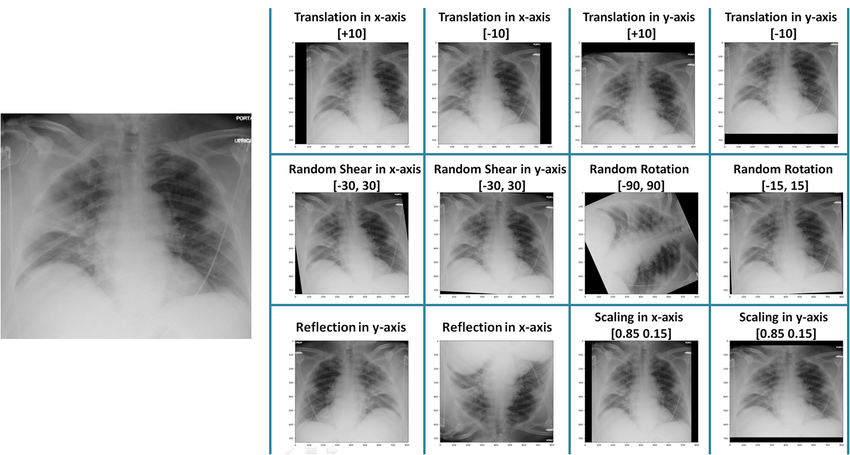
\includegraphics[width=0.9\textwidth]{files/capitoli/3-data-augmentation/assets/geometric-transformations.png}
    \caption{\label{fig:geometric-transformations}Esempi di trasformazioni geometriche applicate ad un'immagine X-ray\cite{34}}
\end{figure}

\subsubsection{Modifiche dei Colori}
Le modifiche dei colori alterano i valori cromatici nell'immagine, aiutando il modello a riconoscere gli oggetti sotto diverse condizioni di illuminazione e colore.

Possiamo andare a modificare:
\begin{itemize}
  \item \textbf{Luminosità}: migliora la capacità del modello di adattarsi a condizioni di luce diverse
  \item \textbf{Saturazione}: aiuta il modello a riconoscere gli oggetti indipendentemente dall'intensità dei colori
  \item \textbf{Contrasto}: permette al modello di distinguere meglio gli oggetti in base alle differenze di luminosità
  \item \textbf{Colore}: aiuta il modello a riconoscere gli oggetti indipendentemente dalle condizioni cromatiche.
\end{itemize}

\begin{figure}[ht]
    \centering
    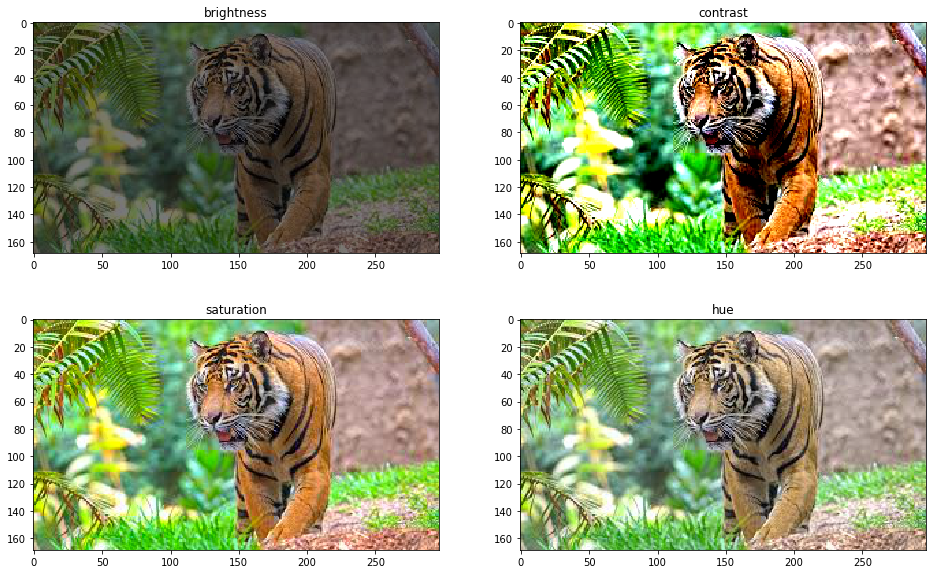
\includegraphics[width=0.8\textwidth]{files/capitoli/3-data-augmentation/assets/color-transformations.png}
    \caption{\label{fig:color-transformations}Esempi di trasformazioni di colore applicate ad una foto\cite{35}}
\end{figure}

\subsubsection{Distorsioni e Rumore}
Le distorsioni e l'aggiunta di rumore all'immagine possono migliorare la robustezza del modello, aiutandolo a imparare a riconoscere gli oggetti anche in condizioni non ideali o con interferenze.

\begin{itemize}
  \item \textbf{Distorsione Elastica}: introduce deformazioni locali all'immagine, aumentando la varietà dei pattern geometrici presenti nei dati di addestramento.
  \item \textbf{Aggiunta di Rumore Gaussiano}: introduce variazioni casuali simili al rumore nei sensori delle fotocamere, migliorando la capacità del modello di distinguere dettagli sottili e rendendolo più robusto contro i disturbi.
  \item \textbf{Aggiunta di Rumore Salt-and-Pepper}: simula interferenze come granelli di polvere o artefatti minori, rendendo il modello più robusto rispetto alle imperfezioni dell'immagine.
  \item \textbf{Blur}: sfoca l'immagine simulando condizioni di scarsa qualità, migliorando la capacità del modello di riconoscere oggetti in condizioni di bassa definizione o in movimento.
  \item \textbf{Distorsione da Lente}: introduce distorsioni ottiche simili a quelle causate da lenti fotografiche, migliorando la capacità del modello di adattarsi a variazioni nelle proporzioni degli oggetti.
\end{itemize}

\vspace{1cm}

\begin{figure}[ht]
    \centering
    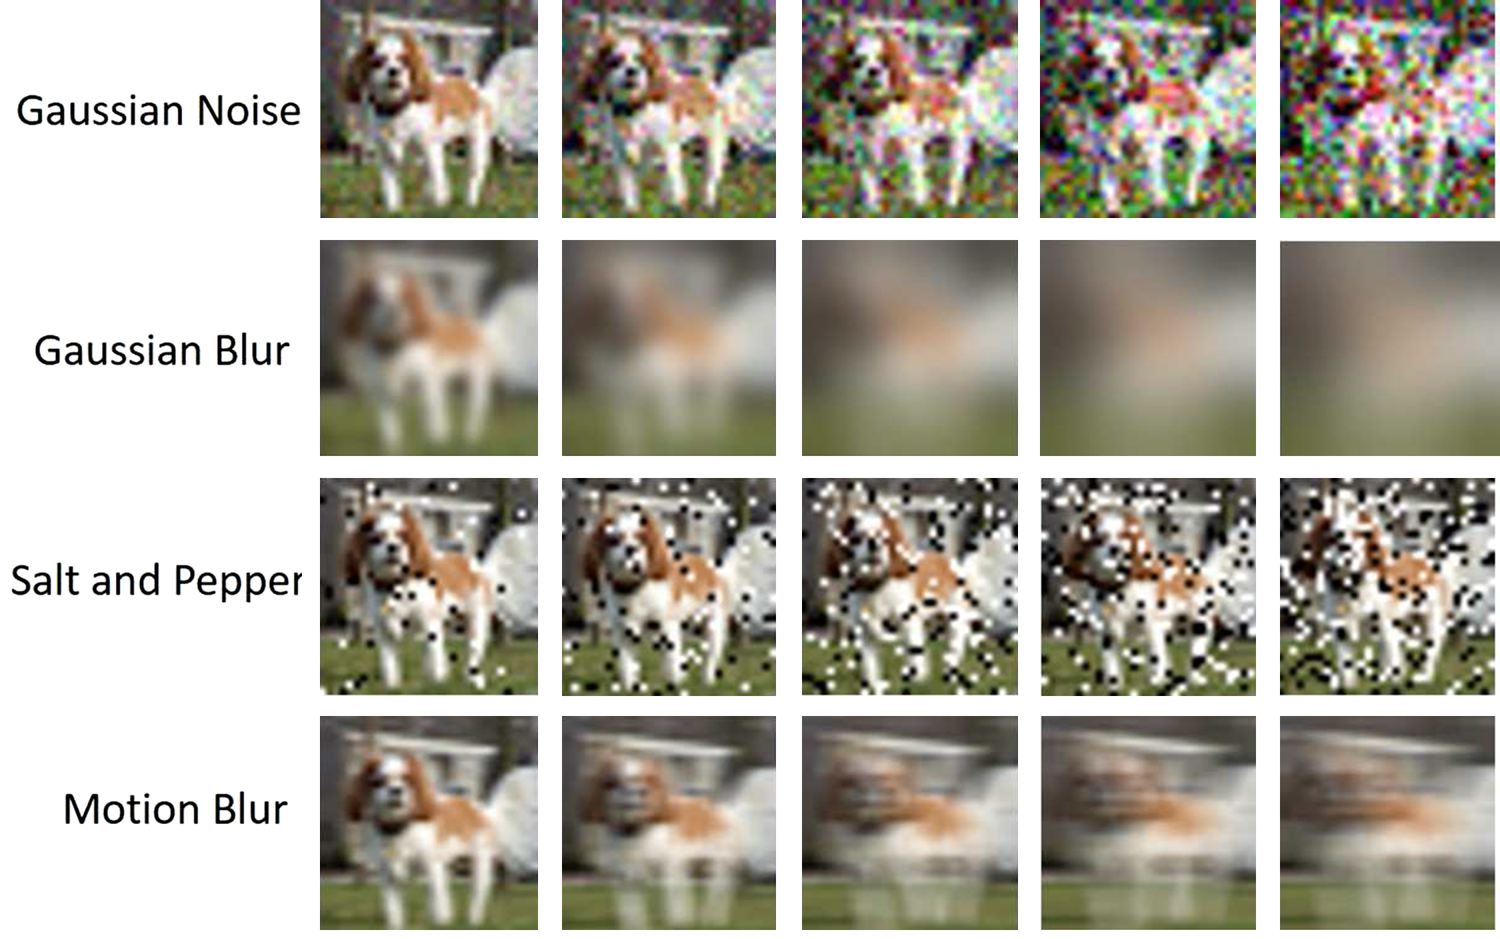
\includegraphics[width=0.8\textwidth]{files/capitoli/3-data-augmentation/assets/distortion-noise.png}
    \caption{\label{fig:distortion-noise}Esempi di distorsioni ed aggiunte di rumore\cite{36}}
\end{figure}

\newpage

\subsection{Tecniche Avanzate di Data Augmentation}
Le tecniche avanzate di data augmentation vanno oltre le trasformazioni geometriche ed i cambiamenti di colore, introducendo strategie più complesse per migliorare le prestazioni dei modelli. Queste tecniche sono progettate per generare dati sintetici più diversificati e realistici, migliorando così la capacità del modello di generalizzare su dati non visti durante l'addestramento.

\subsubsection{Augmentation tramite GAN}
L'Augmentation tramite Generative Adversarial Networks (GAN) è una tecnica che utilizza reti neurali generative e discriminative per generare dati sintetici ad alta fedeltà. Questi modelli apprendono la distribuzione dei dati di input e generano esempi che sono coerenti con tale distribuzione. 

\vspace{0.5cm}

\begin{figure}[ht]
    \centering
    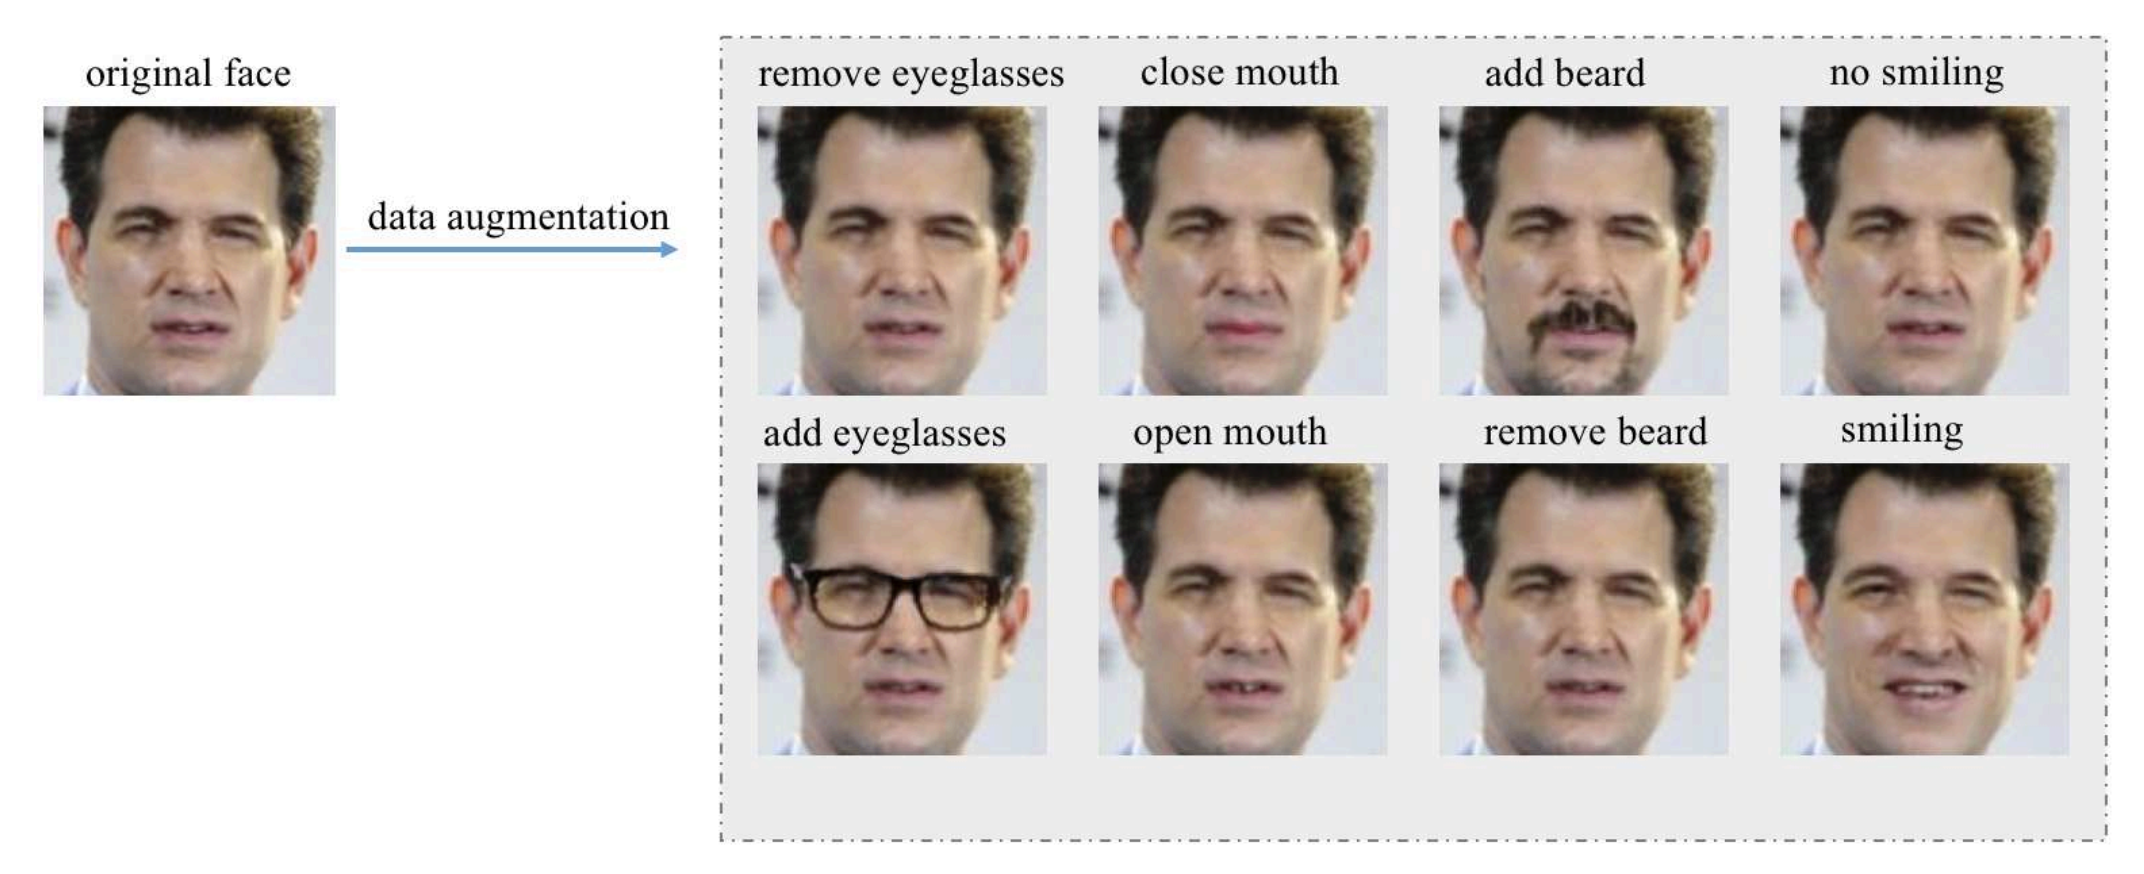
\includegraphics[width=0.9\textwidth]{files/capitoli/3-data-augmentation/assets/gan-augmentation.png}
    \caption{\label{fig:gan-augmentatione}Esempi di immagini generate tramite GAN\cite{37}}
\end{figure}

\newpage

\subsubsection{Mixup, Cutout e Cutmix}
Mixup è una tecnica di data augmentation che mescola coppie di campioni di addestramento per creare nuovi esempi. Questa tecnica combina le immagini e le etichette dei campioni originali per creare nuove istanze durante l'addestramento. D'altra parte, Cutout è una tecnica che consiste nel mascherare casualmente parti delle immagini di addestramento, incoraggiando il modello a focalizzarsi su caratteristiche meno sensibili al rumore. Infine CutMix è una tecnica che unisce le precedenti, ritagliando regioni delle immagini come nel Cutout, ma andandoci ad incollare pezzi di altri esempi. Questa tecnica forza il modello a generalizzare meglio, rendendolo robusto alle distorsioni localizzate e migliorando la sua capacità di rilevare e classificare oggetti anche in presenza di parziali occlusioni.

\vspace{0.5cm}

\begin{figure}[ht]
    \centering
    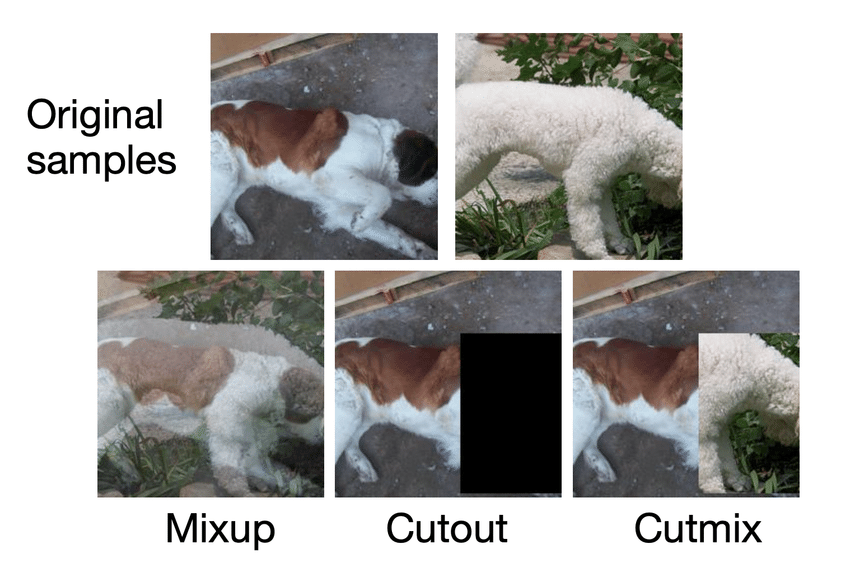
\includegraphics[width=0.8\textwidth]{files/capitoli/3-data-augmentation/assets/mixup-cutout-cutmix.png}
    \caption{\label{fig:gan-augmentatione}Esempi di Mixup, Cutout e Cutmix\cite{38}}
\end{figure}

\newpage
\chapter{Sperimentazione e Risultati}\label{ch:sperimentazione-risultati}

\section{Obiettivo}
L'obiettivo di questa tesi sperimentale è confrontare le prestazioni di tre modelli avanzati di Object Detection applicati alle immagini termiche: YOLOv8, YOLO-World e RT-DETR. Questi modelli sono stati scelti per rappresentare tre diversi approcci al problema del riconoscimento degli oggetti, consentendo così un confronto dettagliato delle loro capacità su questo specifico tipo di dati.

Per massimizzare le prestazioni di questi modelli, espanderemo il dataset di immagini termiche utilizzando tecniche di augmentation, valutando le più efficaci offerte dalla libreria Albumentations. Successivamente, testeremo i tre modelli in questi scenari per identificare quello che meglio si adatta al riconoscimento di oggetti in immagini termiche e, soprattutto, ottiene il miglioramento più significativo grazie all'addestramento su dataset aumentato.

\newpage

\section{Preparazione del dataset}

\subsection{Dataset termico FLIR}
Il dataset termico utilizzato è fornito da Teledyne FLIR\cite{39}, un'azienda leader nel settore delle tecnologie di rilevamento termico e di imaging a infrarossi, ed è stato progettato per consentire agli sviluppatori di avviare l'addestramento di reti neurali convoluzionali, finalizzate alla creazione della prossima generazione di sistemi avanzati di assistenza alla guida (ADAS) e veicoli autonomi più sicuri ed efficienti.

Il dataset è composto da immagini catturate sia di giorno (60\%) che di notte (40\%) su strade e autostrade nell’area di Santa Barbara (California) da Novembre a Maggio, con condizioni meteorologiche sia limpide che nuvolose.

\vspace{0.5cm}

\begin{figure}[ht]
    \centering
    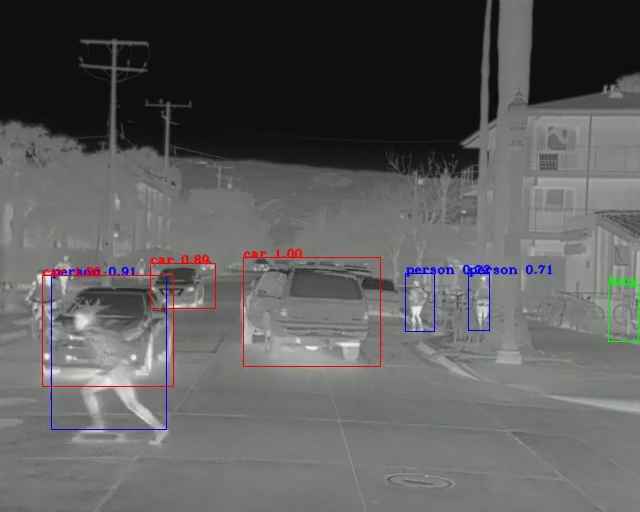
\includegraphics[width=0.8\textwidth]{files/capitoli/4-sperimentazione-risultati/assets/flir-example.png}
    \caption{\label{fig:flir-example}Immagine del dataset termico FLIR\cite{39}}
\end{figure}

\newpage

Le immagini sono state acquisite utilizzando una termocamera con le seguenti specifiche\cite{39}:
\begin{itemize}
    \item \textbf{Termocamera IR}: Tau2 640 x 512, 13 mm f/1,0 (HFOV 45°, VFOV 37°)
    \item \textbf{Telecamera FLIR BlackFly}: (BFS-U3-51S5C-C) 1280 x 1024, ottica megapixel Computar 4-8 mm f/1,4-16 (FOV impostato per Tau2)
\end{itemize}

\subsection{Estrazione e Formattazione dei subset}
Scaricando il dataset dalla apposita pagina di Teledyne FLIR\cite{39}, ci troviamo di fronte alle seguenti raccolte di immagini:

\begin{figure}[ht]
    \centering
    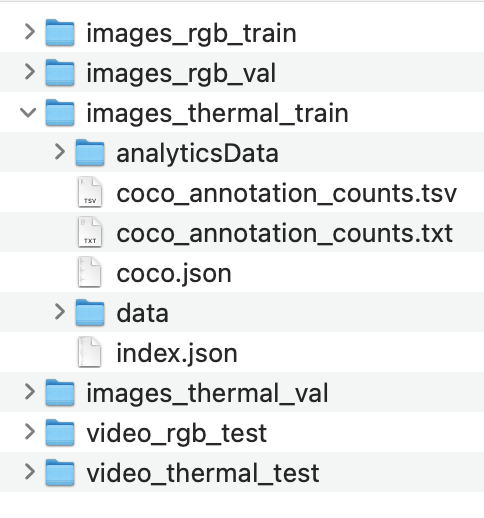
\includegraphics[width=0.35\textwidth]{files/capitoli/4-sperimentazione-risultati/assets/flir-adas.png}
    \caption{\label{fig:flir-adas}Contenuto di FLIR\textunderscore ADAS\textunderscore v2.zip}
\end{figure}

I dati di nostro interesse sono contenuti nelle cartelle relative alle immagini termiche ("thermal") per i 3 subset di train, val e test; le immagini termiche di ogni subset si trovano della cartella \texttt{data}, mentre le annotazioni nei file \texttt{coco.json} (formato MSCOCO) e \texttt{index.json} (formato di Conservator, un tool proprietario di Teledyne FLIR per il management dei dataset).

\newpage

Per addestrare i modelli YOLO, è necessario organizzare la cartella del dataset con la seguente struttura:

\begin{figure}[ht]
    \centering
    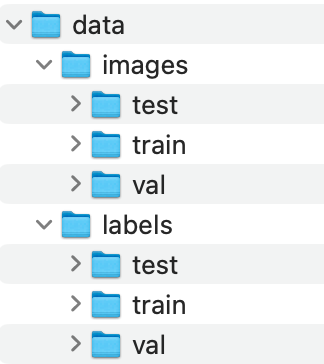
\includegraphics[width=0.23\textwidth]{files/capitoli/4-sperimentazione-risultati/assets/yolo-data-format.png}
    \caption{\label{fig:yolo-data-format}Struttura cartella dataset per i modelli YOLO}
\end{figure}

Tramite uno script Python sono quindi andato a copiare le immagini dei tre subset nelle relative cartelle in \texttt{data/images}, e successivamente sono andato a generare le annotazioni in formato YOLO di ciascuna immagine partendo da quelle presenti in \texttt{index.json}, inserendole in file di testo salvati in \texttt{data/labels}.

Perciò ciascuna immagine \texttt{(frameID).jpg} in \texttt{data/images/(subset)}, avrà il corrispettivo file di testo \texttt{(frameID).txt} in \texttt{data/labels/(subset)}, il quale contiene le relative annotazioni nel formato YOLO: ogni riga corrisponde ad una Bounding Box e contiene id della classe, coordinata X del centro, coordinata Y del centro, larghezza ed altezza.

\vspace{0.5cm}

\begin{figure}[ht]
    \centering
    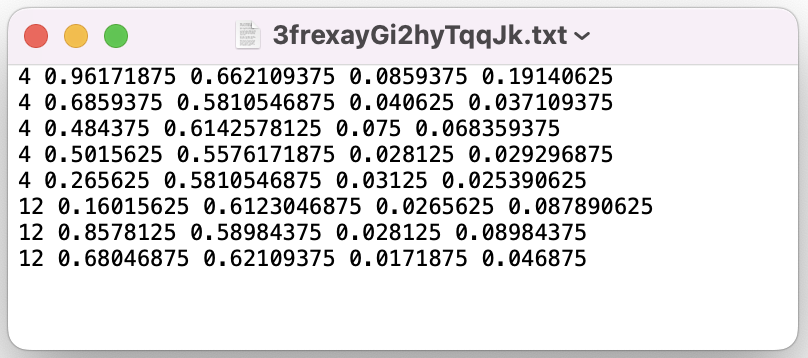
\includegraphics[width=0.7\textwidth]{files/capitoli/4-sperimentazione-risultati/assets/label-example.png}
    \caption{\label{fig:label-example}File contenente le annotazioni del frame "3frexayGi2hyTqqJk"}
\end{figure}


\subsection{Analisi delle classi}
Il dataset originario contiene le annotazioni relative a 20 classi di oggetti, segue l'analisi dettagliata del numero di annotazioni presenti nei 3 subset per ciascuna delle classi:

\begin{figure}[ht]
    \centering
    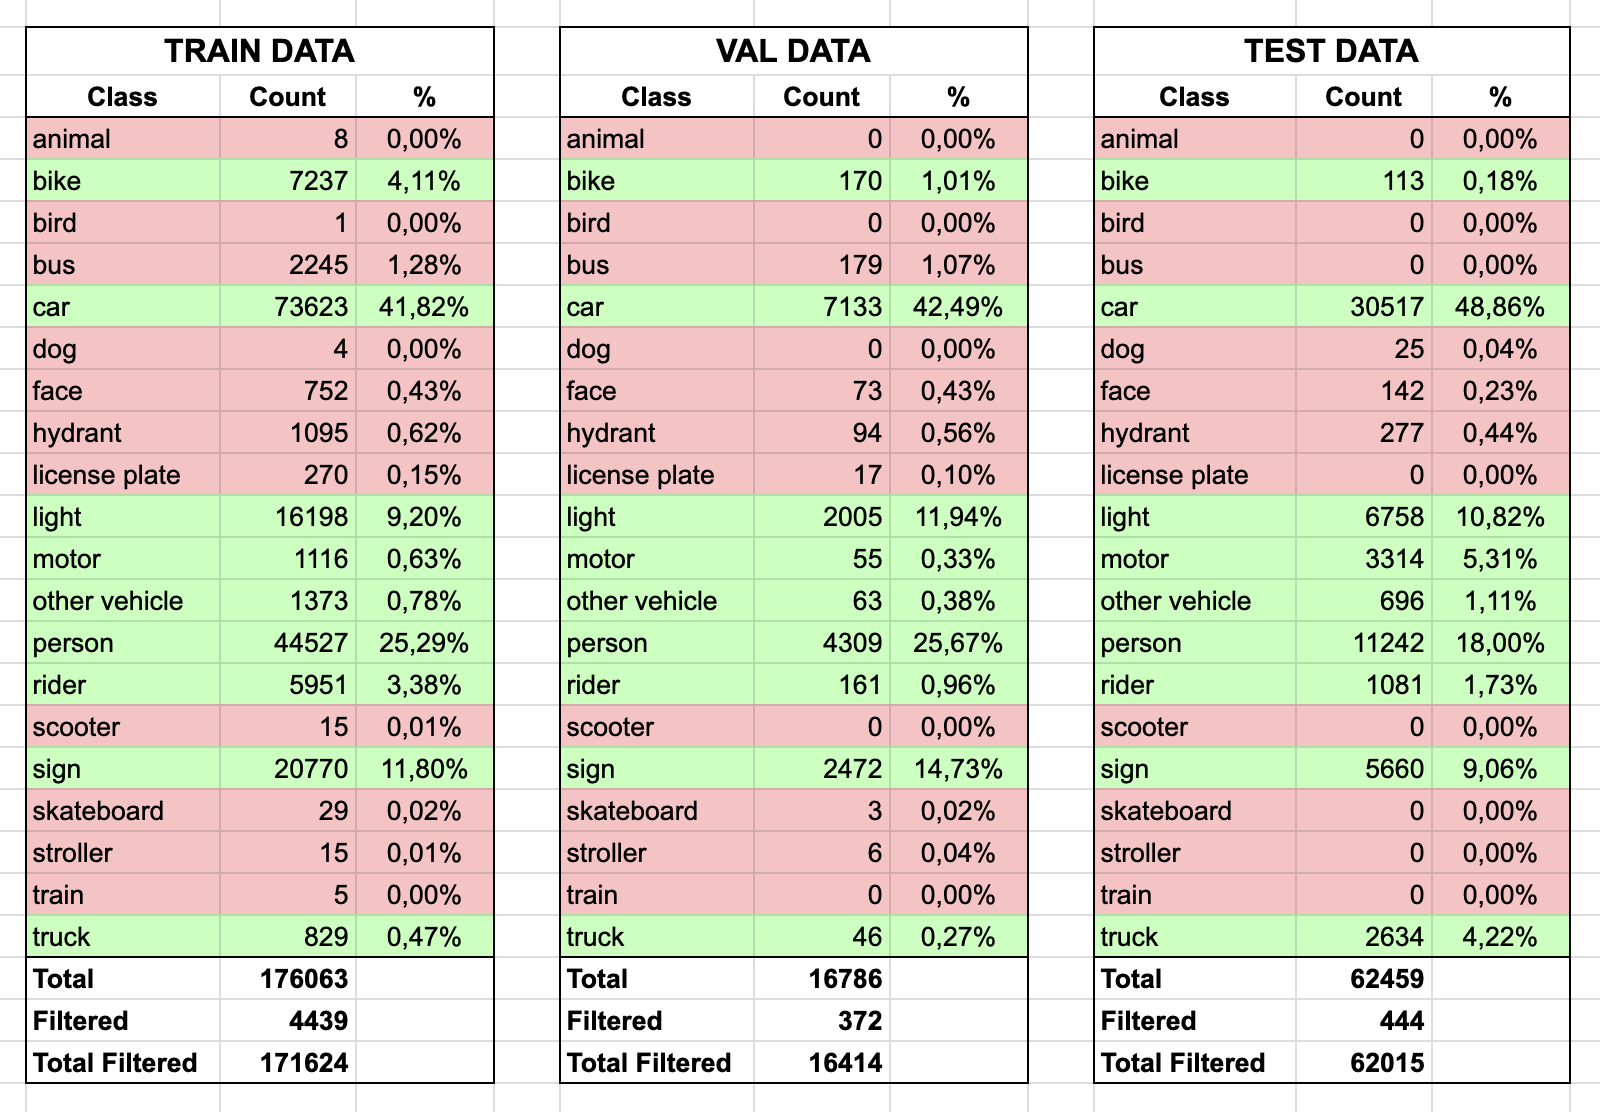
\includegraphics[width=1\textwidth]{files/capitoli/4-sperimentazione-risultati/assets/class-counts.png}
    \caption{\label{fig:class-counts}Analisi delle annotazioni per ciascuna classe}
\end{figure}

Possiamo notare che alcune classi sono sottorappresentate nelle annotazioni rispetto al totale, il che potrebbe compromettere l'efficacia dell'addestramento del modello e deteriorare le metriche di valutazione complessive.
Per questo motivo, ho deciso di filtrare le classi in questione dalle annotazioni del dataset (quelle evidenziate in rosso).

\newpage

\subsection{Nuovo dataset filtrato}
Ho quindi generato un nuovo dataset chiamato \texttt{filtered-data}, che contiene le stesse immagini dell'originale, ma con i file .txt delle annotazioni aggiornati. Le annotazioni sono state filtrate tramite uno script Python che ha scansionato le righe dei file di annotazione originali, rimuovendo quelle relative alle classi da escludere.

Così facendo, ho ottenuto il dataset su cui addestrare i modelli, suddiviso come segue:
\begin{itemize}
    \item \textbf{Train subset}: 10742 esempi
    \item \textbf{Val subset}: 1144 esempi
    \item \textbf{Test subset}: 3749 esempi
\end{itemize}

\newpage


\section{Modelli di partenza}

\subsection{Ultralytics}
Ultralytics\cite{40} è un'azienda leader nello sviluppo di soluzioni avanzate di Computer Vision e Deep Learning. Conosciuta principalmente per il suo contributo alla famiglia di modelli YOLO, Ultralytics si distingue per la creazione di strumenti di rilevamento oggetti ad alte prestazioni, ampiamente utilizzati in varie applicazioni industriali e di ricerca. La piattaforma di Ultralytics fornisce modelli pre-addestrati e strumenti di facile utilizzo per l'implementazione rapida di algoritmi di object detection, garantendo prestazioni elevate e scalabilità.

\subsection{Modelli di Ultralytics utilizzati}
Per questo esperimento sono stati scelti i modelli più piccoli per ognuna delle tre tipologie di modello, caratterizzati da una ridotta complessità in termini di numero di parametri da dover addestrare.

I modelli in questione sono:
\begin{itemize}
    \item \textbf{yolov8n}: modello YOLOv8 "nano"\cite{27}
    \item \textbf{yolov8s-world}: modello YOLOv8 "small-world"\cite{30}
    \item \textbf{rtdetr-l}: modello RT-DETR "large"\cite{32}
\end{itemize}

La scelta di questi modelli è stata guidata dalla necessità di avere modelli leggeri e veloci da addestrare, in modo da ottimizzare il processo di sperimentazione e ottenere risultati rapidi senza compromettere significativamente la precisione.

\newpage

\subsection{Valutazione dei modelli}
Per valutare le prestazioni dei modelli ho utilizzato il metodo \texttt{val}\cite{41} fornito da Ultralytics, il quale analizza il comportamento di un determinato modello sul subset specificato nel file di configurazione, fornendo una serie di metriche utili. Il test avviene tramite il seguente script Python, in cui il file di configurazione \texttt{test-config.yaml} specifica al metodo di valutare il modello sul subset di test: 

\begin{figure}[ht]
    \centering
    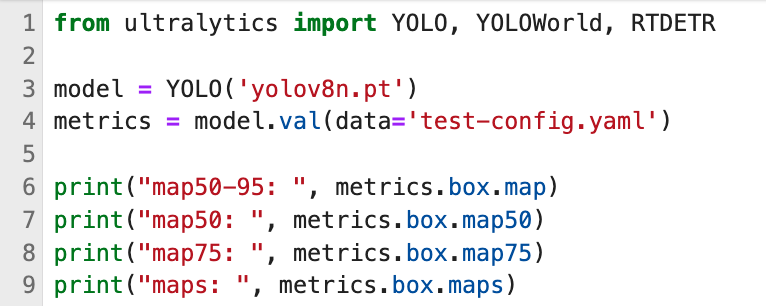
\includegraphics[width=0.5\textwidth]{files/capitoli/4-sperimentazione-risultati/assets/test-script.png}
    \caption{\label{fig:test-script}Script per il testing di 'yolov8n'}
\end{figure}

\subsubsection{Metriche}
Valutare l'efficacia dei modelli di Object Detection richiede l'uso di metriche precise che misurino la capacità del modello di individuare e localizzare correttamente gli oggetti all'interno delle immagini. Le seguenti metriche fondamentali sono essenziali per questa valutazione:

\begin{itemize}
    \item \textbf{Precision}: misura la proporzione di oggetti predetti correttamente rispetto a tutti gli oggetti predetti dal modello.
    \item \textbf{Recall}: misura la proporzione di oggetti veri positivi rilevati correttamente rispetto a tutti gli oggetti veri positivi presenti nel dataset.
    \item \textbf{Average Precision (AP)}: calcola l'area sotto la curva Precision-Recall (PR curve), riflettendo la precisione del modello al variare della soglia di confidenza delle predizioni
    \item \textbf{Intersection over Union (IoU)}: misura la sovrapposizione tra la bounding box predetta e quella ground-truth, ed è calcolato come area dell'intersezione divisa per area dell'unione delle due bounding box.
\end{itemize}

\begin{figure}[ht]
    \centering
    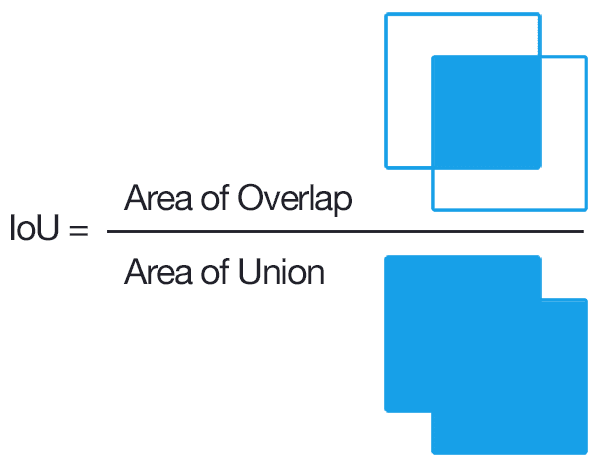
\includegraphics[width=0.4\textwidth]{files/capitoli/4-sperimentazione-risultati/assets/iou.png}
    \caption{\label{fig:iou}Intersection over Union\cite{42}}
\end{figure}

Per valutare più efficacemente le prestazioni dei modelli utilizziamo le metriche di Mean Average Precision (mAP), che rappresentano la media delle Average Precision calcolate per ogni classe:

\begin{itemize}
    \item \textbf{mAP50-95}: media dell'Average Precision (AP) calcolata su diverse soglie di IoU (Intersection over Union), dall'50\% al 95\%
    \item \textbf{mAP50}: media dell'Average Precision (AP) calcolata con IoU al 50\%
    \item \textbf{mAP75}: media dell'Average Precision (AP) calcolata con IoU al 75\%
\end{itemize}

Queste metriche ci forniranno una misura dettagliata delle capacità del modello nel rilevare e localizzare correttamente gli oggetti all'interno delle immagini, considerando diverse soglie di sovrapposizione tra le predizioni del modello e le ground-truth bounding box.

\newpage

\subsection{Test dei modelli non addestrati}

Prima di procedere con l'addestramento dei tre modelli, ho valutato le loro prestazioni iniziali sul dataset filtrato, ottenendo i seguenti risultati:

\begin{figure}[ht]
    \centering
    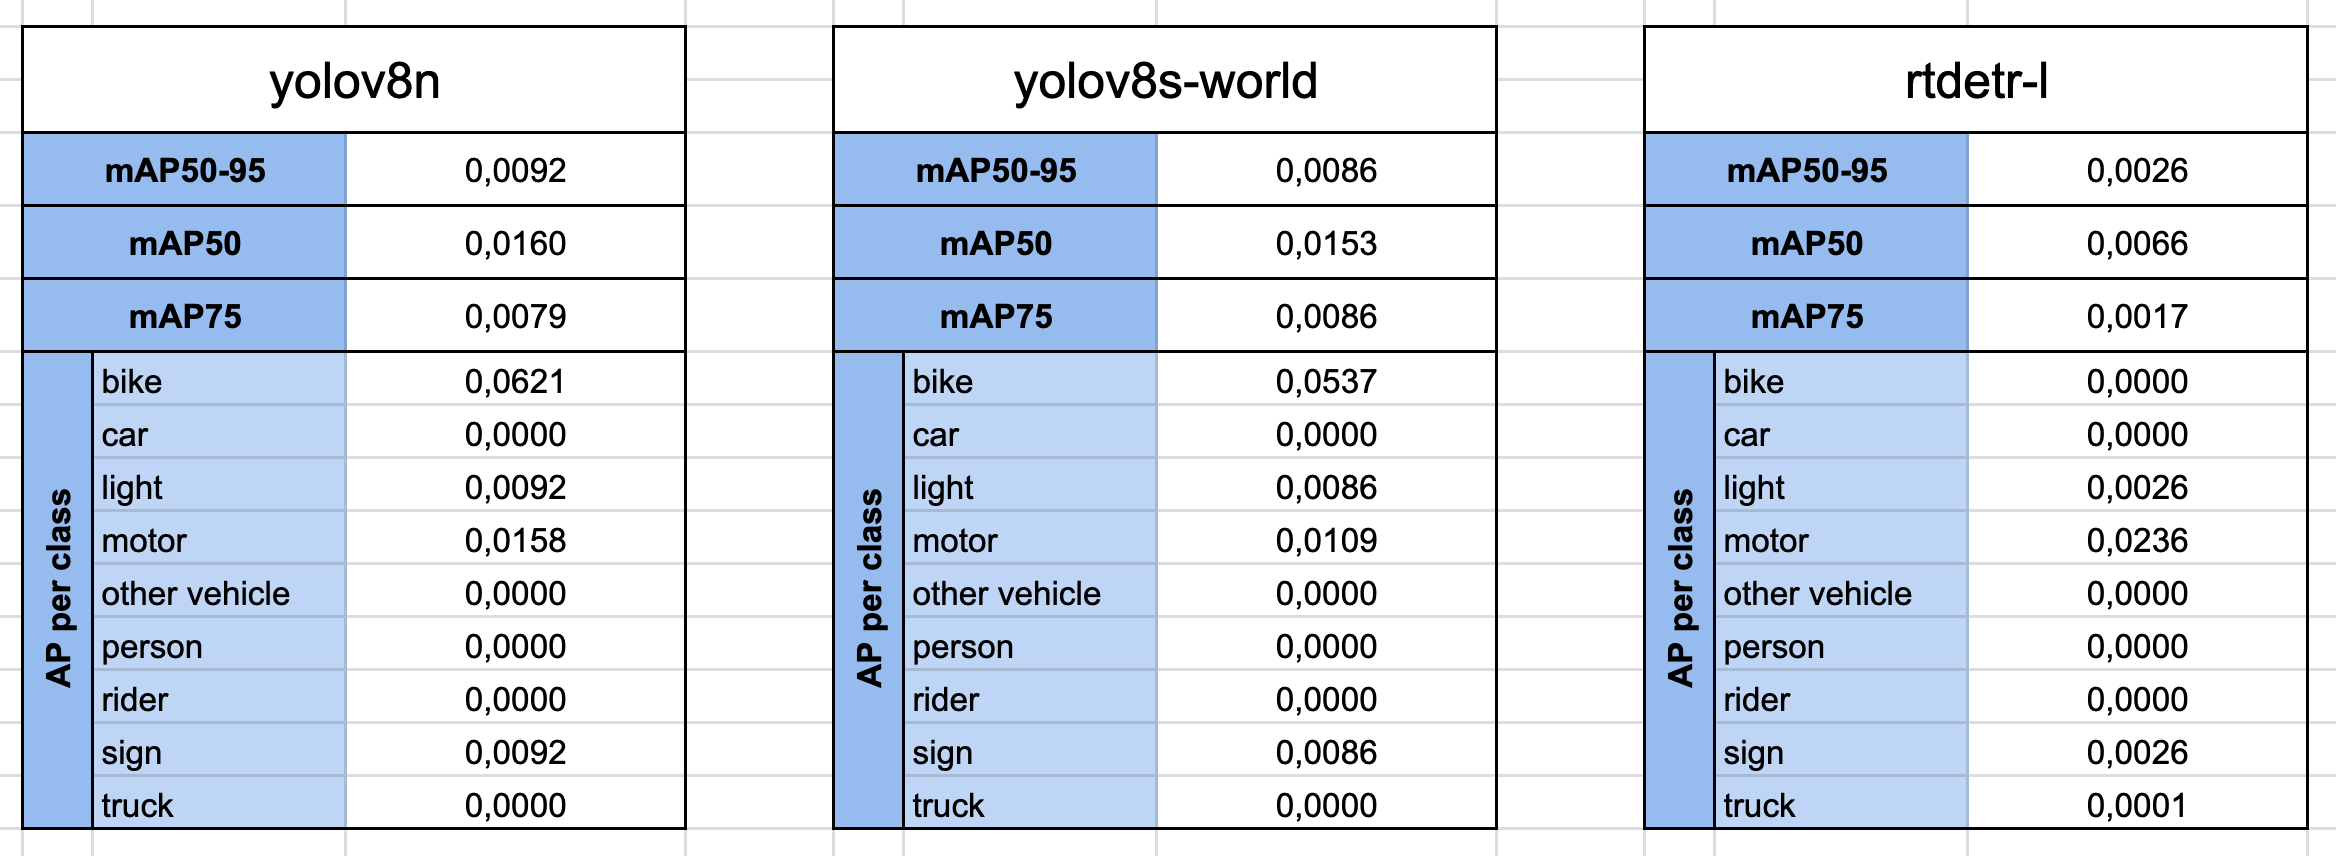
\includegraphics[width=1\textwidth]{files/capitoli/4-sperimentazione-risultati/assets/untrained-metrics.png}
    \caption{\label{fig:untrained-metrics}Risultati test dei modelli non addestrati}
\end{figure}

Possiamo osservare che senza un'ottimizzazione specifica (fine-tuning) sul dataset di immagini termiche, i modelli presentano prestazioni inadeguate nell'Object Detection di questi dati, evidenziando metriche significativamente inferiori rispetto a quelle ottenute sui dataset standard (come COCO) riportate da Ultralytics.

\begin{figure}[ht]
    \centering
    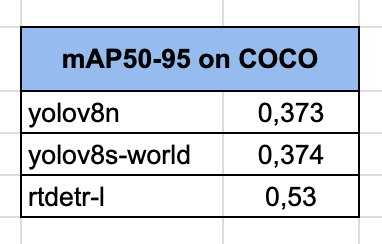
\includegraphics[width=0.3\textwidth]{files/capitoli/4-sperimentazione-risultati/assets/coco-maps.png}
    \caption{\label{fig:coco-maps}mAP50-95 dei modelli su dataset COCO}
\end{figure}

\clearpage

\begin{figure}[ht]
    \centering
    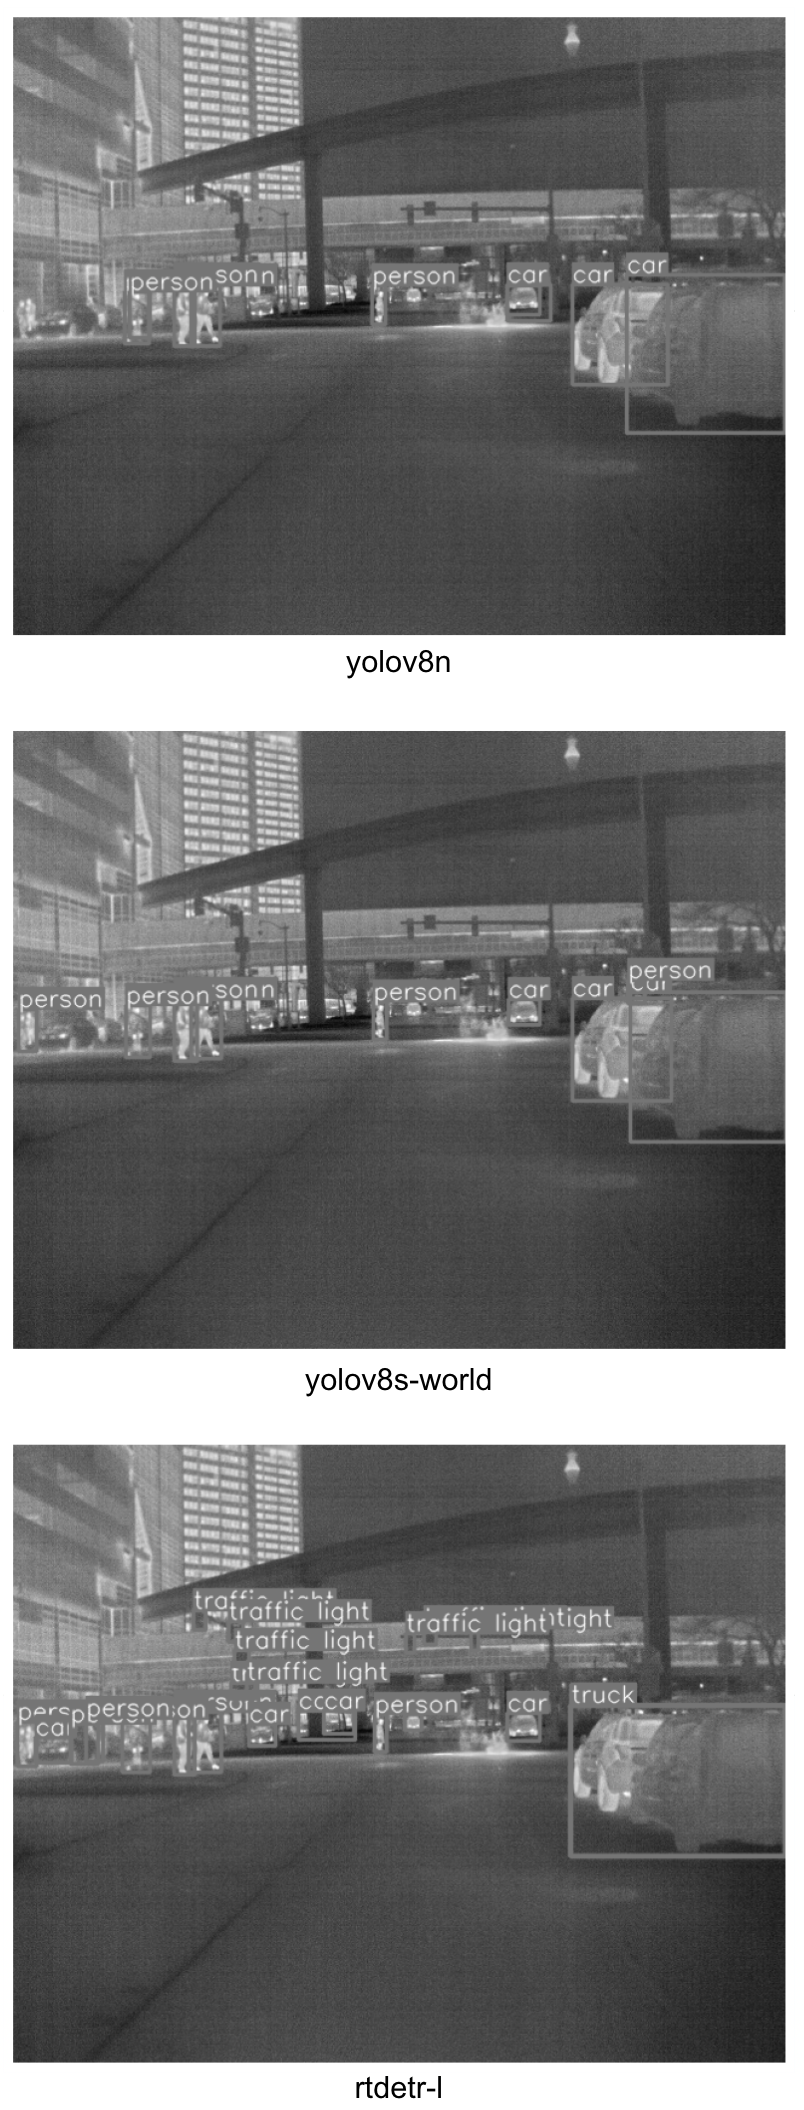
\includegraphics[width=0.6\textwidth]{files/capitoli/4-sperimentazione-risultati/assets/initial-detections.png}
    \caption{\label{fig:initial-detections}Detections effettutate dai modelli non addestrati}
\end{figure}

\clearpage

\section{Addestramento su dataset filtrato}

\subsection{Addestramento dei modelli}

L'addestramento dei tre modelli è stato effettuato tramite uno script Python che impiega la libreria di Ultralytics per caricare ed addestrare il modello:

\begin{figure}[ht]
    \centering
    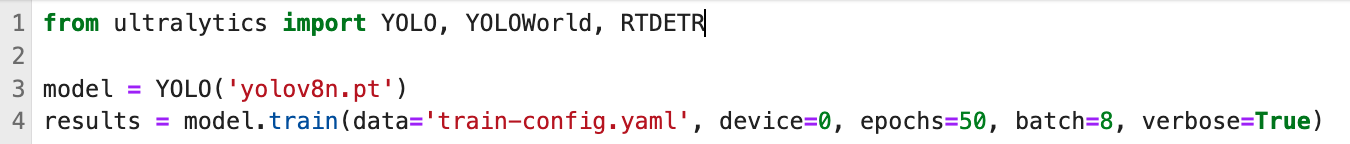
\includegraphics[width=1\textwidth]{files/capitoli/4-sperimentazione-risultati/assets/train-script.png}
    \caption{\label{fig:train-script}Script per l'addestramento di 'yolov8n'}
\end{figure}

\subsubsection{Parametri}
Il metodo \texttt{train}\cite{43} dei modelli di Ultralytics permette di configurare una vasta varietà di parametri, quelli di nostro interesse sono:
\begin{itemize}
    \item \textbf{data}: path al file di configurazione del dataset, in cui vengono specificati il path dei dati e le classi su cui addestrare il modello. In questo caso \texttt{train-config.yaml} indica i path ai subset train e val
    \item \textbf{device}: specifica il dispositivo/i computazionali per l'addestramento
    \item \textbf{epochs}: numero totale delle epochs di addestramento. Ciascuna epoch rappresenta un passaggio completo sull'intero dataset, perciò modificare questo valore influenza la durata dell'addestramento e le prestazioni del modello.
    \item \textbf{batch}: numero di campioni di addestramento processati simultaneamente durante ogni iterazione. Aumentare il batch size può migliorare l'efficienza computazionale, ma richiede più memoria.
    \item \textbf{verbose}: abilita un output dettagliato durante l'addestramento, fornendo log dettagliati e aggiornamenti sul progresso
\end{itemize}

\subsubsection{Augmentations}
Il metodo \texttt{train} di ultralytics implementa internamente delle tecniche di augmentation, essenziali per migliorare la robustezza e le prestazioni dei modelli YOLO. Durante l'addestramento vengono quindi eseguite le seguenti tecniche:

\begin{itemize}
    \item Adjustment of Hue
    \item Adjustment of Saturation
    \item Adjustment of Brightness
    \item Translation
    \item Scaling
    \item Horizontal Flipping
    \item Mixup
    \item Cutout
    \item Crop
\end{itemize}

\newpage

\subsection{Test dei modelli addestrati sul dataset filtrato}
Il primo addestramento dei modelli è stato condotto sul dataset \texttt{filtered-data} per un totale di 50 epochs, in modo da ottenere un buon equilibrio tra velocità di addestramento e capacità del modello; il batch size è stato impostato ad 8 per evitare problemi di memoria sui dispositivi.

Dopo aver completato l'addestramento, ho testato i modelli utilizzando il metodo \texttt{val} sulla migliore configurazione dei parametri interni ottenuta durante le 50 epochs di addestramento, ottenendo i seguenti risultati:

\begin{figure}[ht]
    \centering
    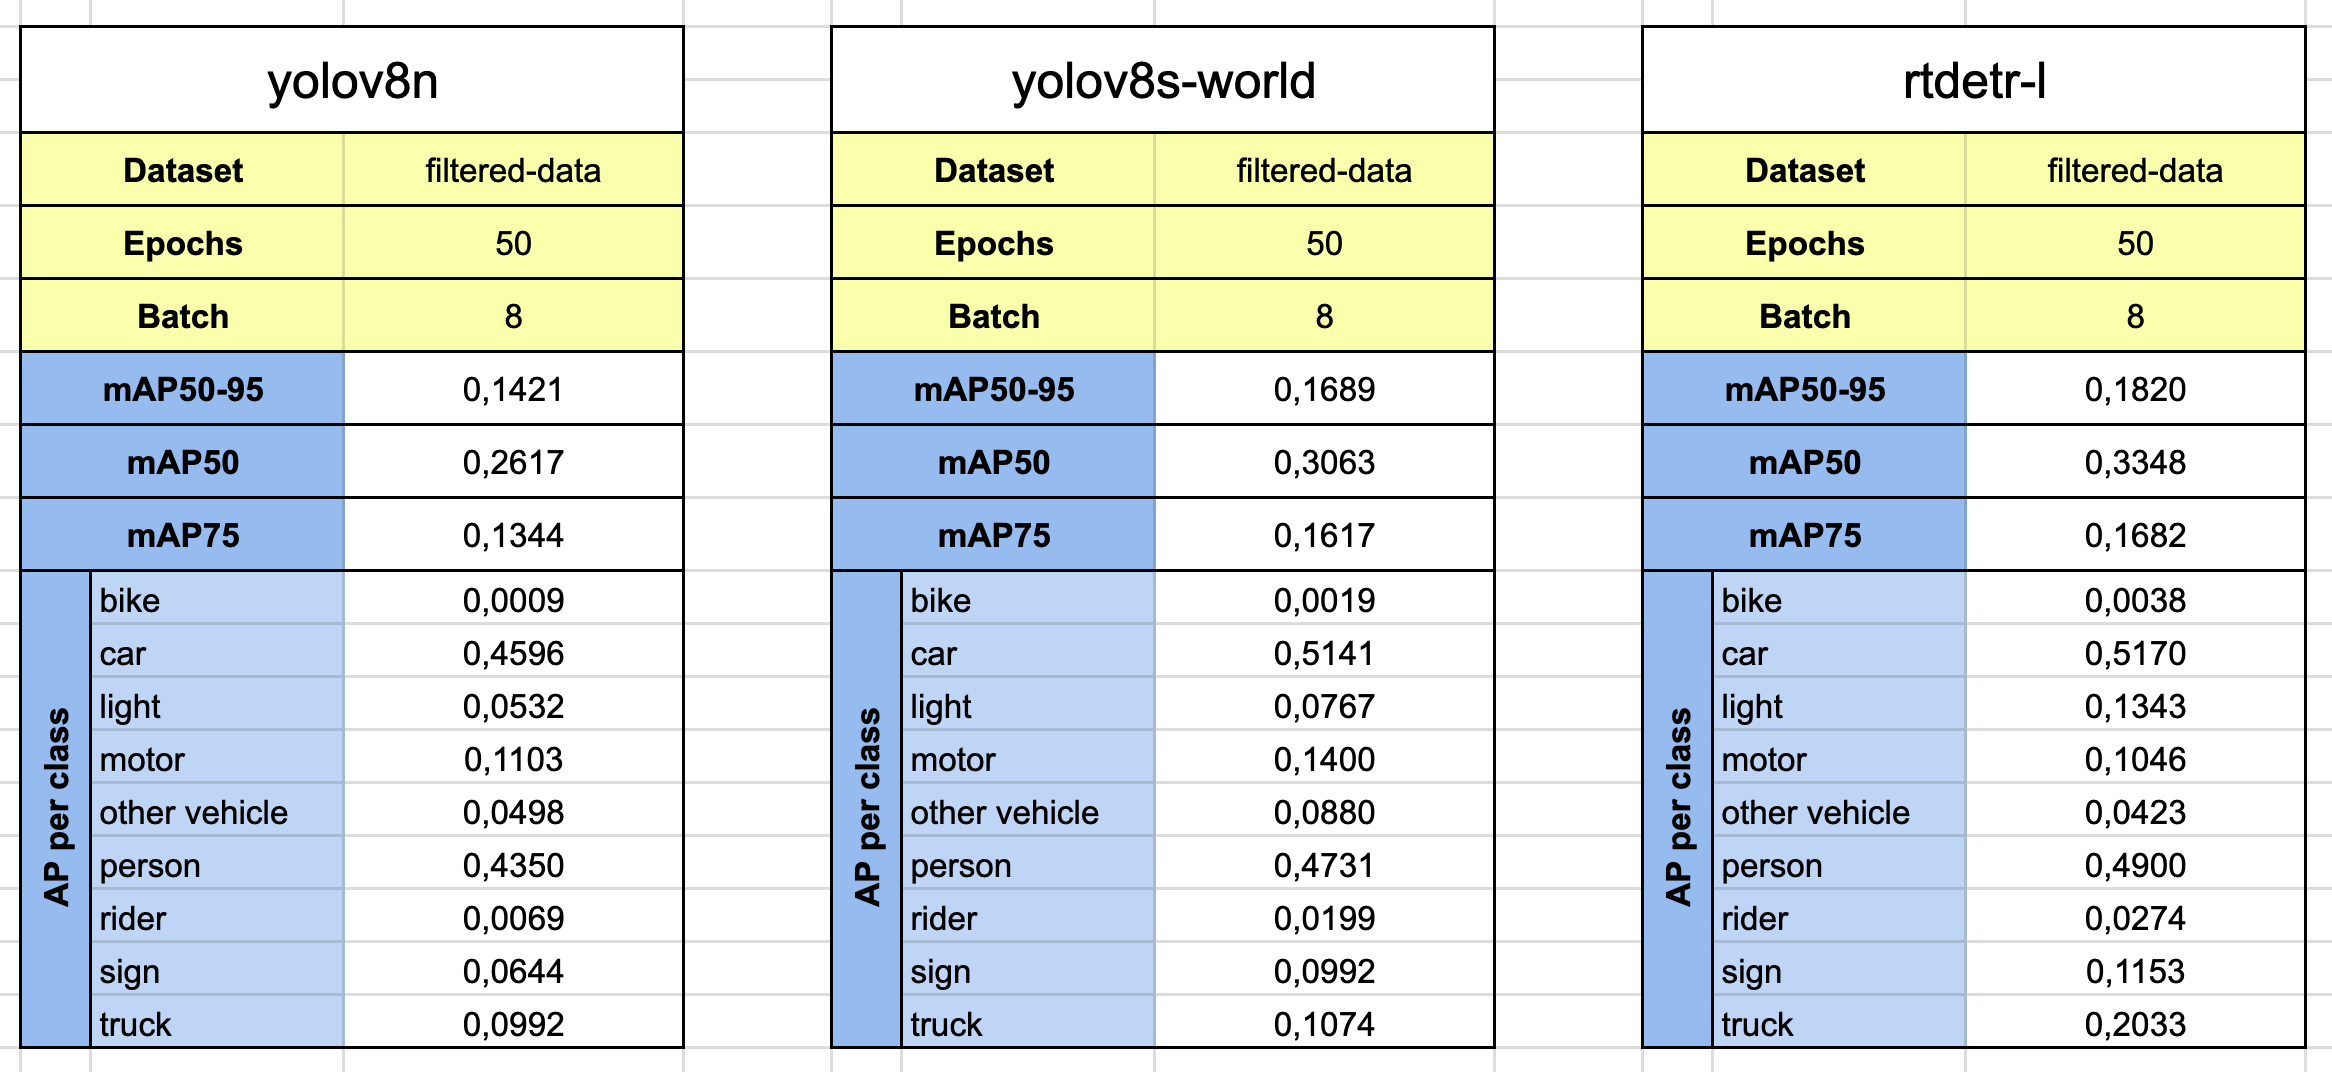
\includegraphics[width=1\textwidth]{files/capitoli/4-sperimentazione-risultati/assets/filtered-data-metrics.png}
    \caption{\label{fig:filtered-data-metrics}Risultati test dei modelli addestrati sul dataset filtrato}
\end{figure}

Possiamo osservare un notevole miglioramento delle prestazioni rispetto ai test precedenti dei modelli, già con questo primo addestramento effettuato su \texttt{filtered-data}.
Questo dimostra come il fine-tuning sia essenziale per ottimizzare i modelli su tipologie di dati specifiche come le nostre immagini termiche.

\clearpage

\begin{figure}[ht]
    \centering
    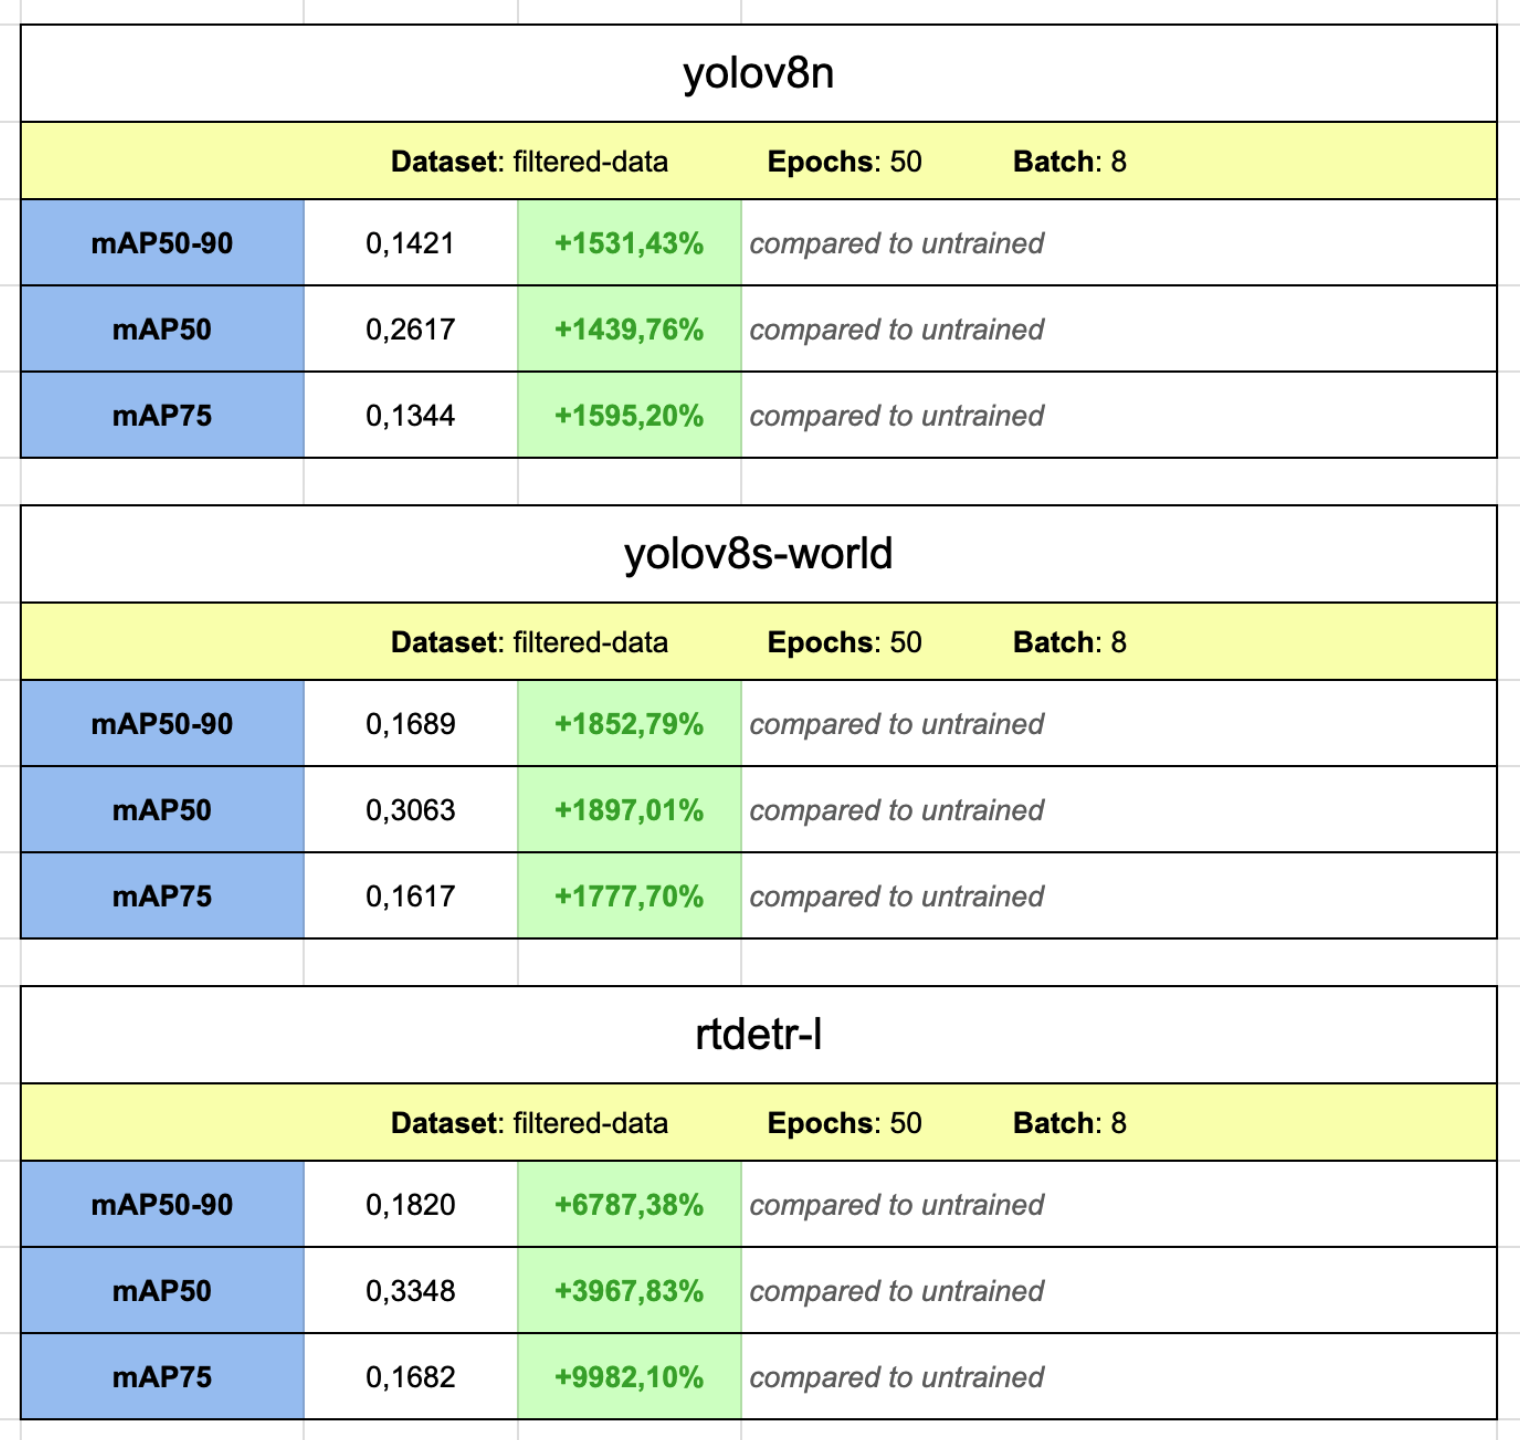
\includegraphics[width=0.9\textwidth]{files/capitoli/4-sperimentazione-risultati/assets/filtered-data-compare.png}
    \caption{\label{fig:filtered-data-compare}Confronto tra i risultati dei test dei modelli addestrati sul dataset filtrato e quelli dei precedenti test}
\end{figure}

\clearpage

\begin{figure}[ht]
    \centering
    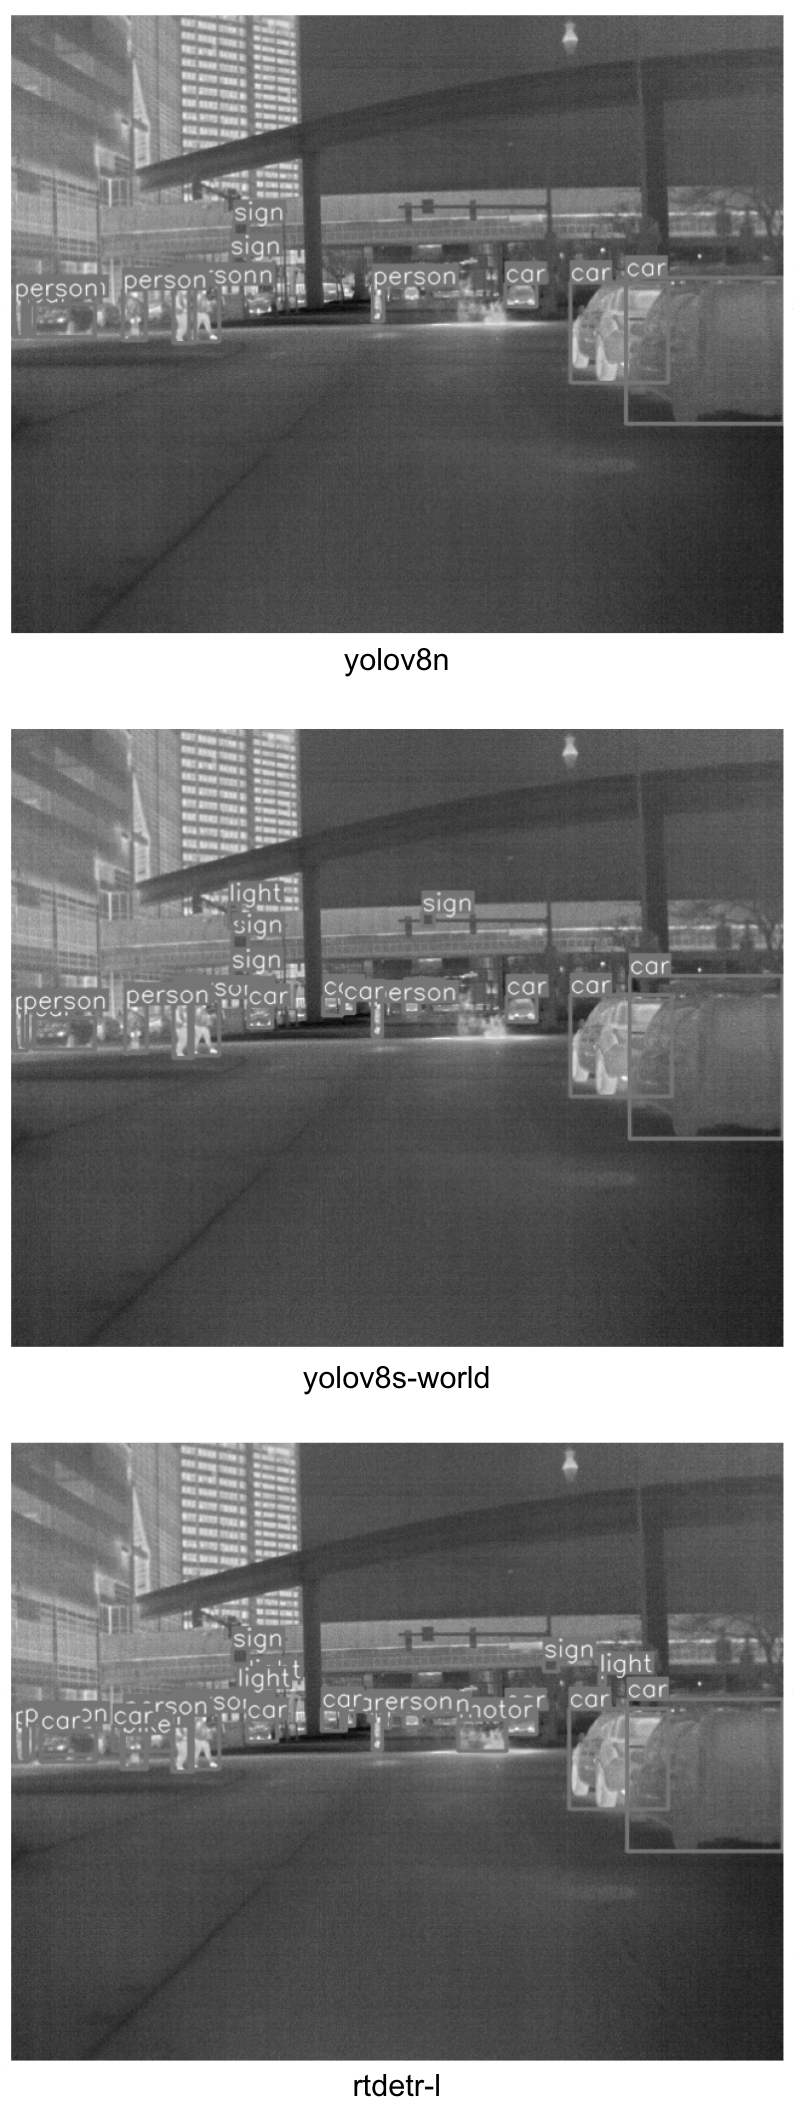
\includegraphics[width=0.6\textwidth]{files/capitoli/4-sperimentazione-risultati/assets/filtered-data-detections.png}
    \caption{\label{fig:initial-detections}Detections effettutate dai modelli addestrati sul dataset filtrato}
\end{figure}

\clearpage
\section{Addestramento su dataset aumentato}
Dopo aver ottenuto risultati significativi dal fine-tuning sul dataset filtrato, il passo successivo è stato individuare una serie di tecniche di augmentation da applicare al dataset. Per questo scopo, ho scelto di utilizzare la libreria Albumentations, che mi ha permesso di generare una versione aumentata del dataset. L'obiettivo era ampliare il subset di training e migliorare ulteriormente le prestazioni dei modelli.

\subsection{Albumentations}
Albumentations\cite{44} è una libreria open-source per l'augmentation delle immagini, progettata principalmente per il deep learning e l'addestramento di modelli di intelligenza artificiale. Essa offre un'ampia gamma di trasformazioni per le immagini, permettendo agli sviluppatori di migliorare la diversità dei dati di addestramento senza modificare manualmente le immagini originali. Le trasformazioni supportate includono modifiche di colore, traslazioni, rotazioni, crop, cambiamenti prospettici, aggiunta di rumore e molto altro ancora. Albumentations è particolarmente apprezzata per la sua velocità e flessibilità, essendo ottimizzata per gestire grandi quantità di dati e integrarsi senza problemi con framework di deep learning come PyTorch e TensorFlow. Nel nostro caso la libreria è stata utilizzata per generare direttamente tramite uno script nuovi dataset aumentati.

\newpage

\subsection{Prima Data Augmentation}

\subsubsection{Primo dataset aumentato}
Ho fatto un primo tentativo di data augmentation sul dataset filtrato, andando a generare una versione "augmented" di ciascuna immagine presente in \texttt{filtered-data/images/train}. Questo è stato fatto tramite uno script Python che applica le seguenti trasformazioni di Albumentations ad ogni immagine: 

\begin{figure}[ht]
    \centering
    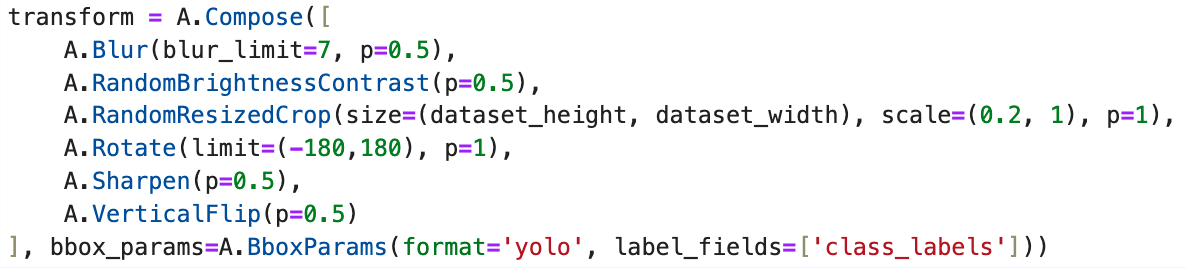
\includegraphics[width=0.9\textwidth]{files/capitoli/4-sperimentazione-risultati/assets/transform-1.png}
    \caption{\label{fig:transform-1}Definizione della trasformazione di Albumentations da applicare alle immagini}
\end{figure}

Il metodo \texttt{transform} di Albumentations consente l'applicazione di un insieme specifico di trasformazioni su un'immagine, gestendo probabilità e intervalli definiti. Questo processo genera una nuova immagine trasformata con relative annotazioni aggiornate, poiché le coordinate delle bounding box possono variare o essere rimosse a seguito delle trasformazioni.
A questo punto, le nuove immagini e annotazioni vengono utilizzate per creare il nuovo dataset aumentato \texttt{augmented-data-1}, il quale avrà esattamente il doppio degli esempi nel subset di training rispetto a \texttt{filtered-data}: 10.742 immagini del dataset originale e 10.742 immagini trasformate.
I subset val e test rimangono invariati.

\clearpage

\begin{figure}[ht]
    \centering
    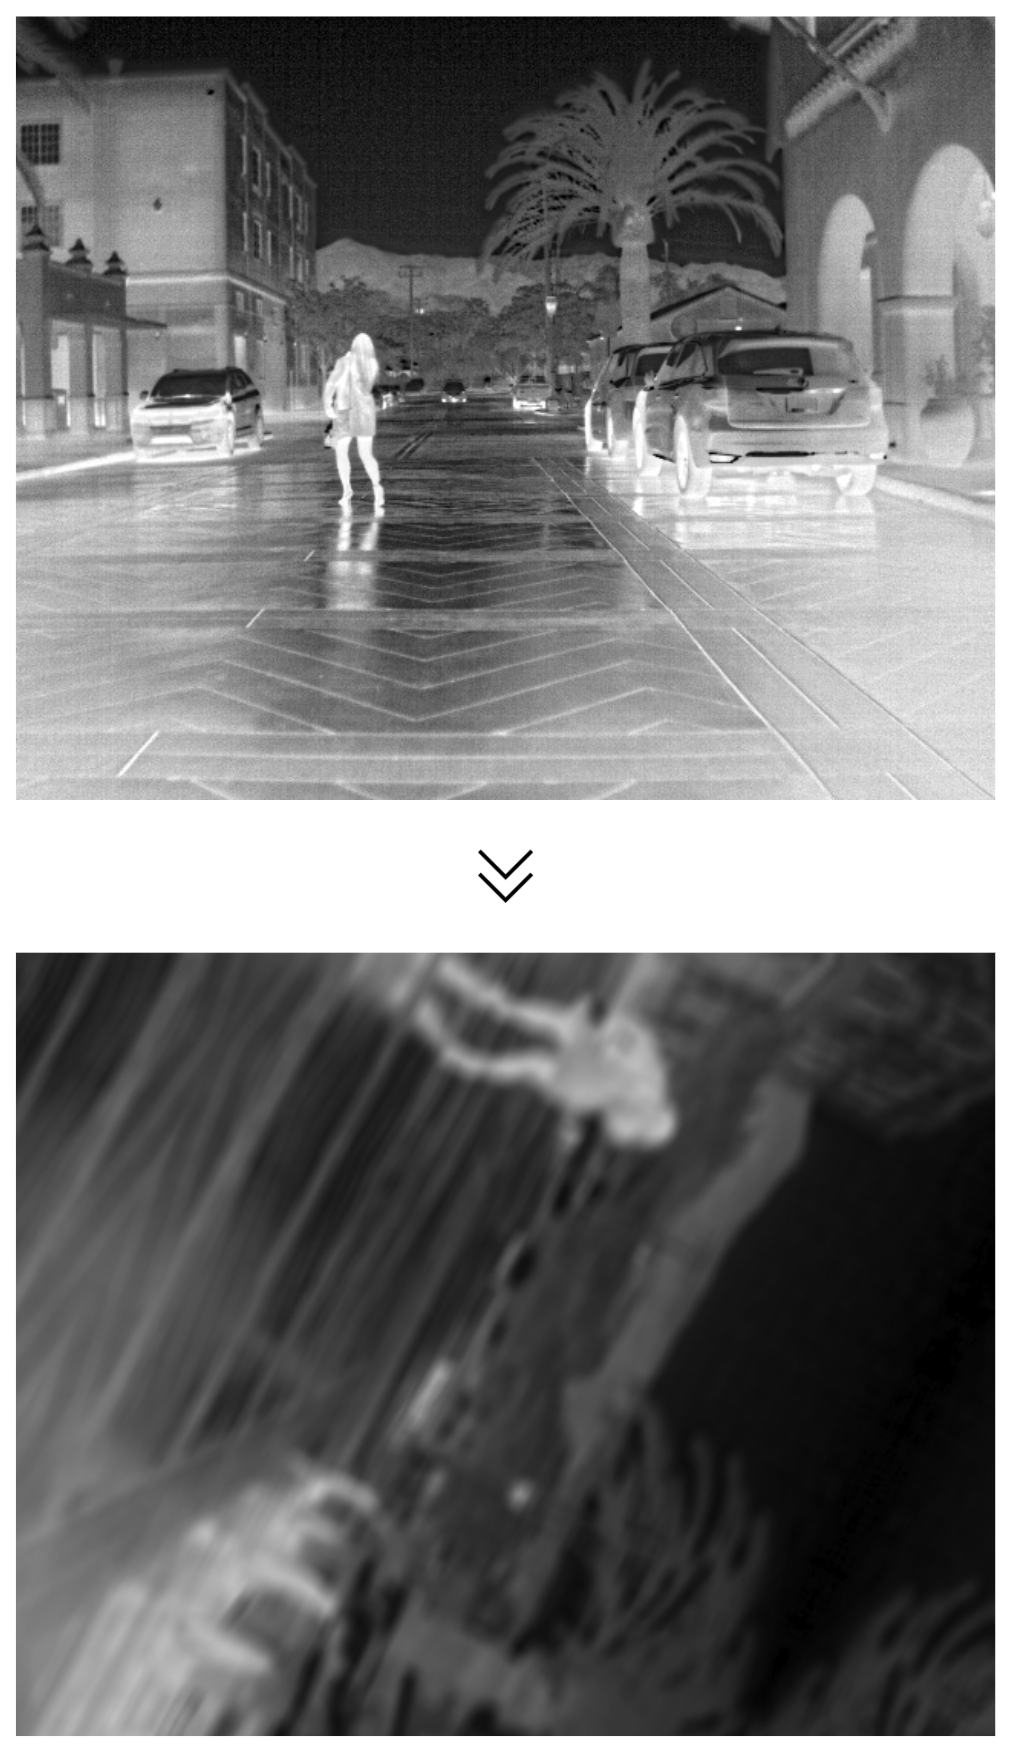
\includegraphics[width=0.8\textwidth]{files/capitoli/4-sperimentazione-risultati/assets/augmented-data-1-example.png}
    \caption{\label{fig:augmented-data-1-example}Esempio di immagine trasformata con la prima data augmentation}
\end{figure}

\clearpage

\subsubsection{Test modelli addestrati sul primo dataset aumentato}
Il secondo addestramento dei modelli è stato quindi condotto sul dataset \texttt{augmented-data-1}, mantenendo le stesse condizioni del primo, con 50 epochs e un batch size di 8.
I successivi test hanno prodotto i seguenti risultati:

\begin{figure}[ht]
    \centering
    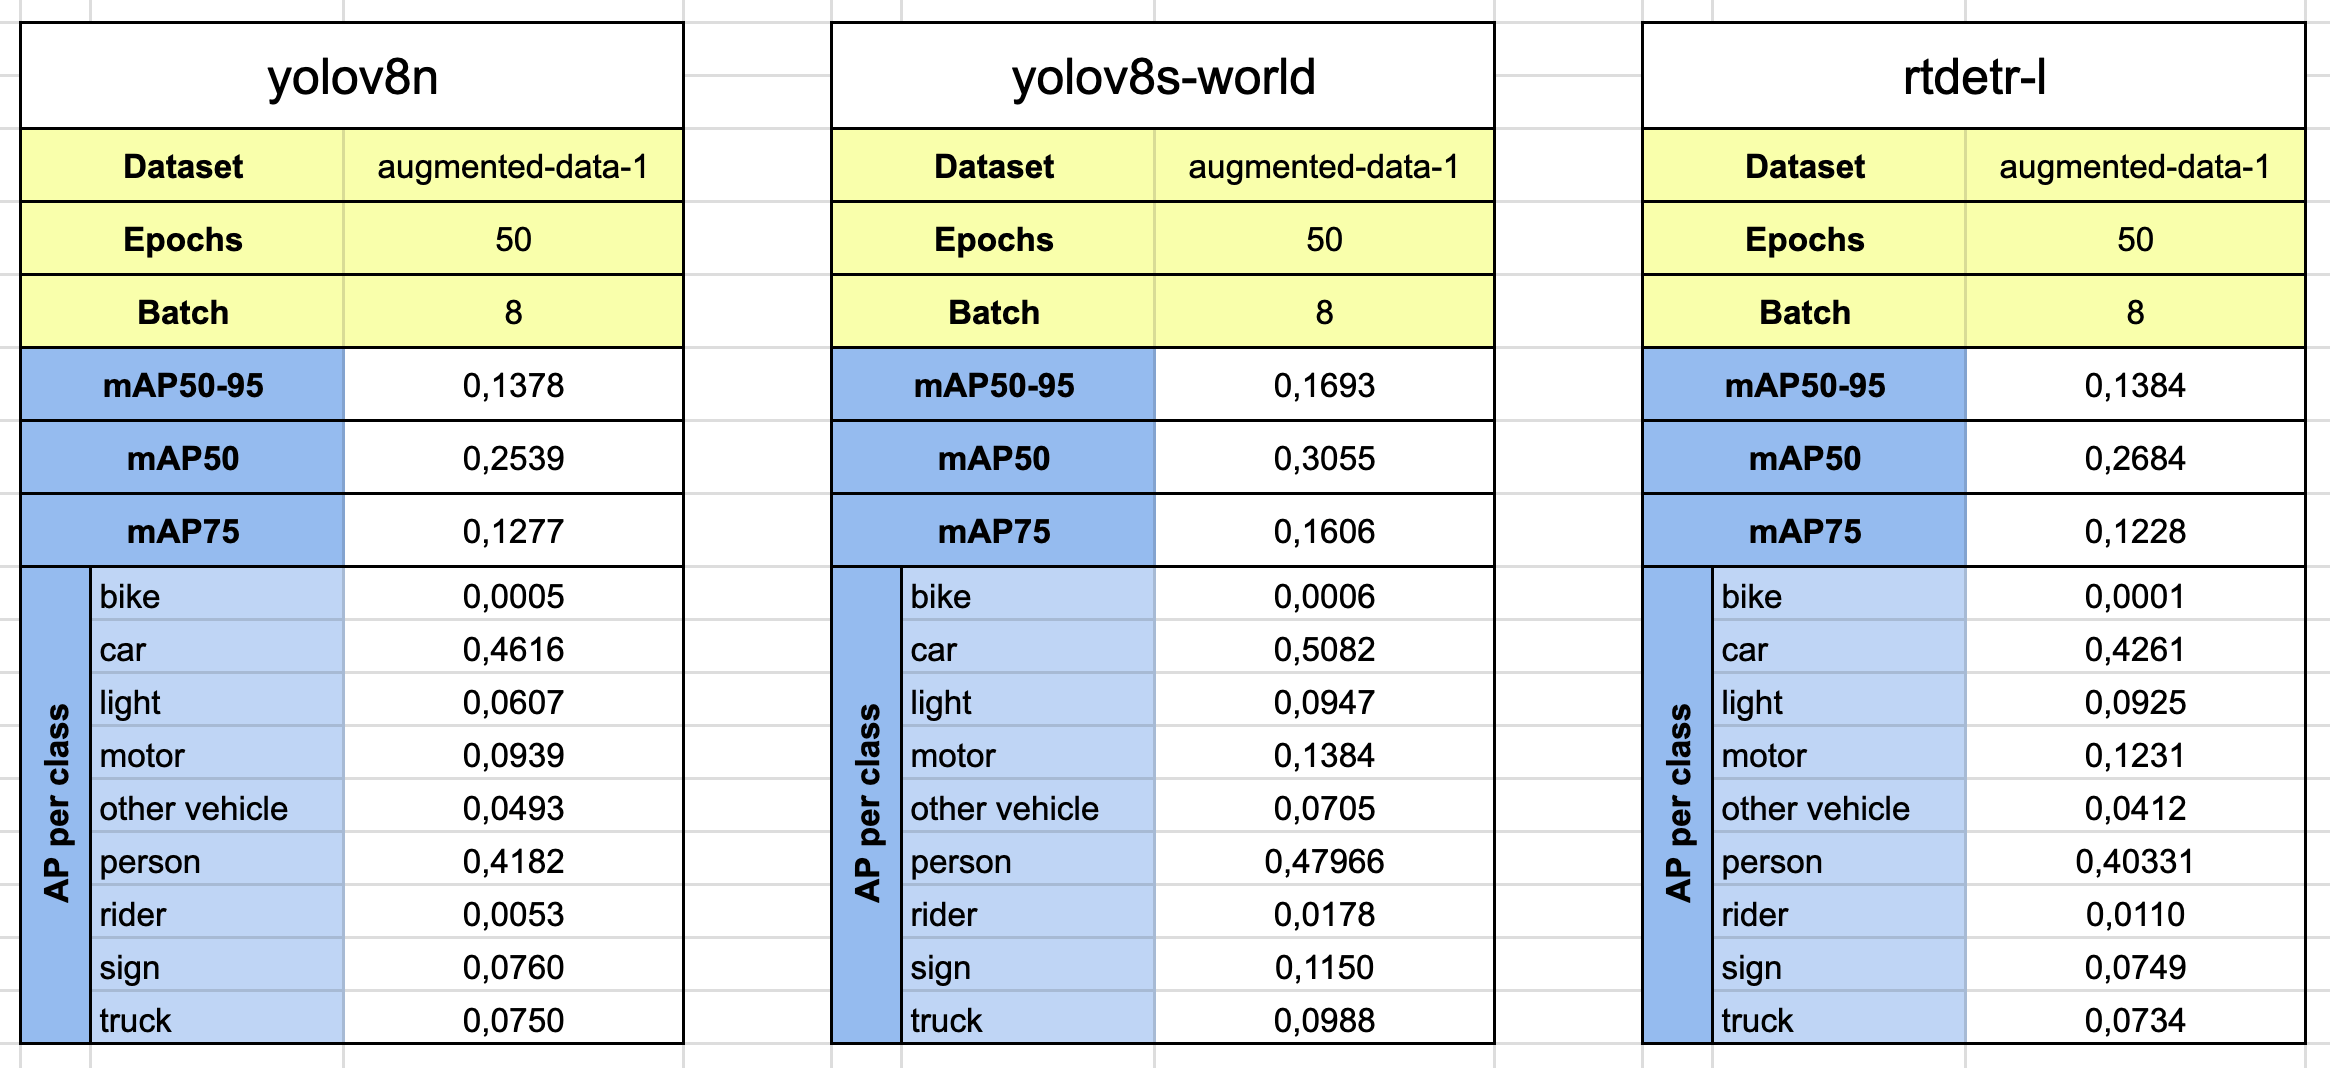
\includegraphics[width=1\textwidth]{files/capitoli/4-sperimentazione-risultati/assets/augmented-data-1-metrics.png}
    \caption{\label{fig:augmented-data-1-metrics}Risultati test dei modelli addestrati sul primo dataset aumentato}
\end{figure}

Notiamo che tutte le metriche, ad eccezione della mAP50-90 di YOLO-World, sono peggiorate con l'addestramento sul dataset aumentato; da questo evinciamo che la combinazione di trasformazioni utilizzate come augmentations è stata inefficace. Ciò è dovuto al fatto che alcune o tutte le trasformazioni erano inadeguate per il contesto delle immagini termiche: potrebbero aver modificato eccessivamente l'immagine o applicato trasformazioni incoerenti rispetto al dataset originario, come il Vertical Flip o la Rotation con un range di 180 gradi, compromettendo il "significato" delle immagini (ad esempio ribaltando macchine o altri elementi stradali, cosa che non accade nei dati catturati dalle termocamere).

\clearpage

\begin{figure}[ht]
    \centering
    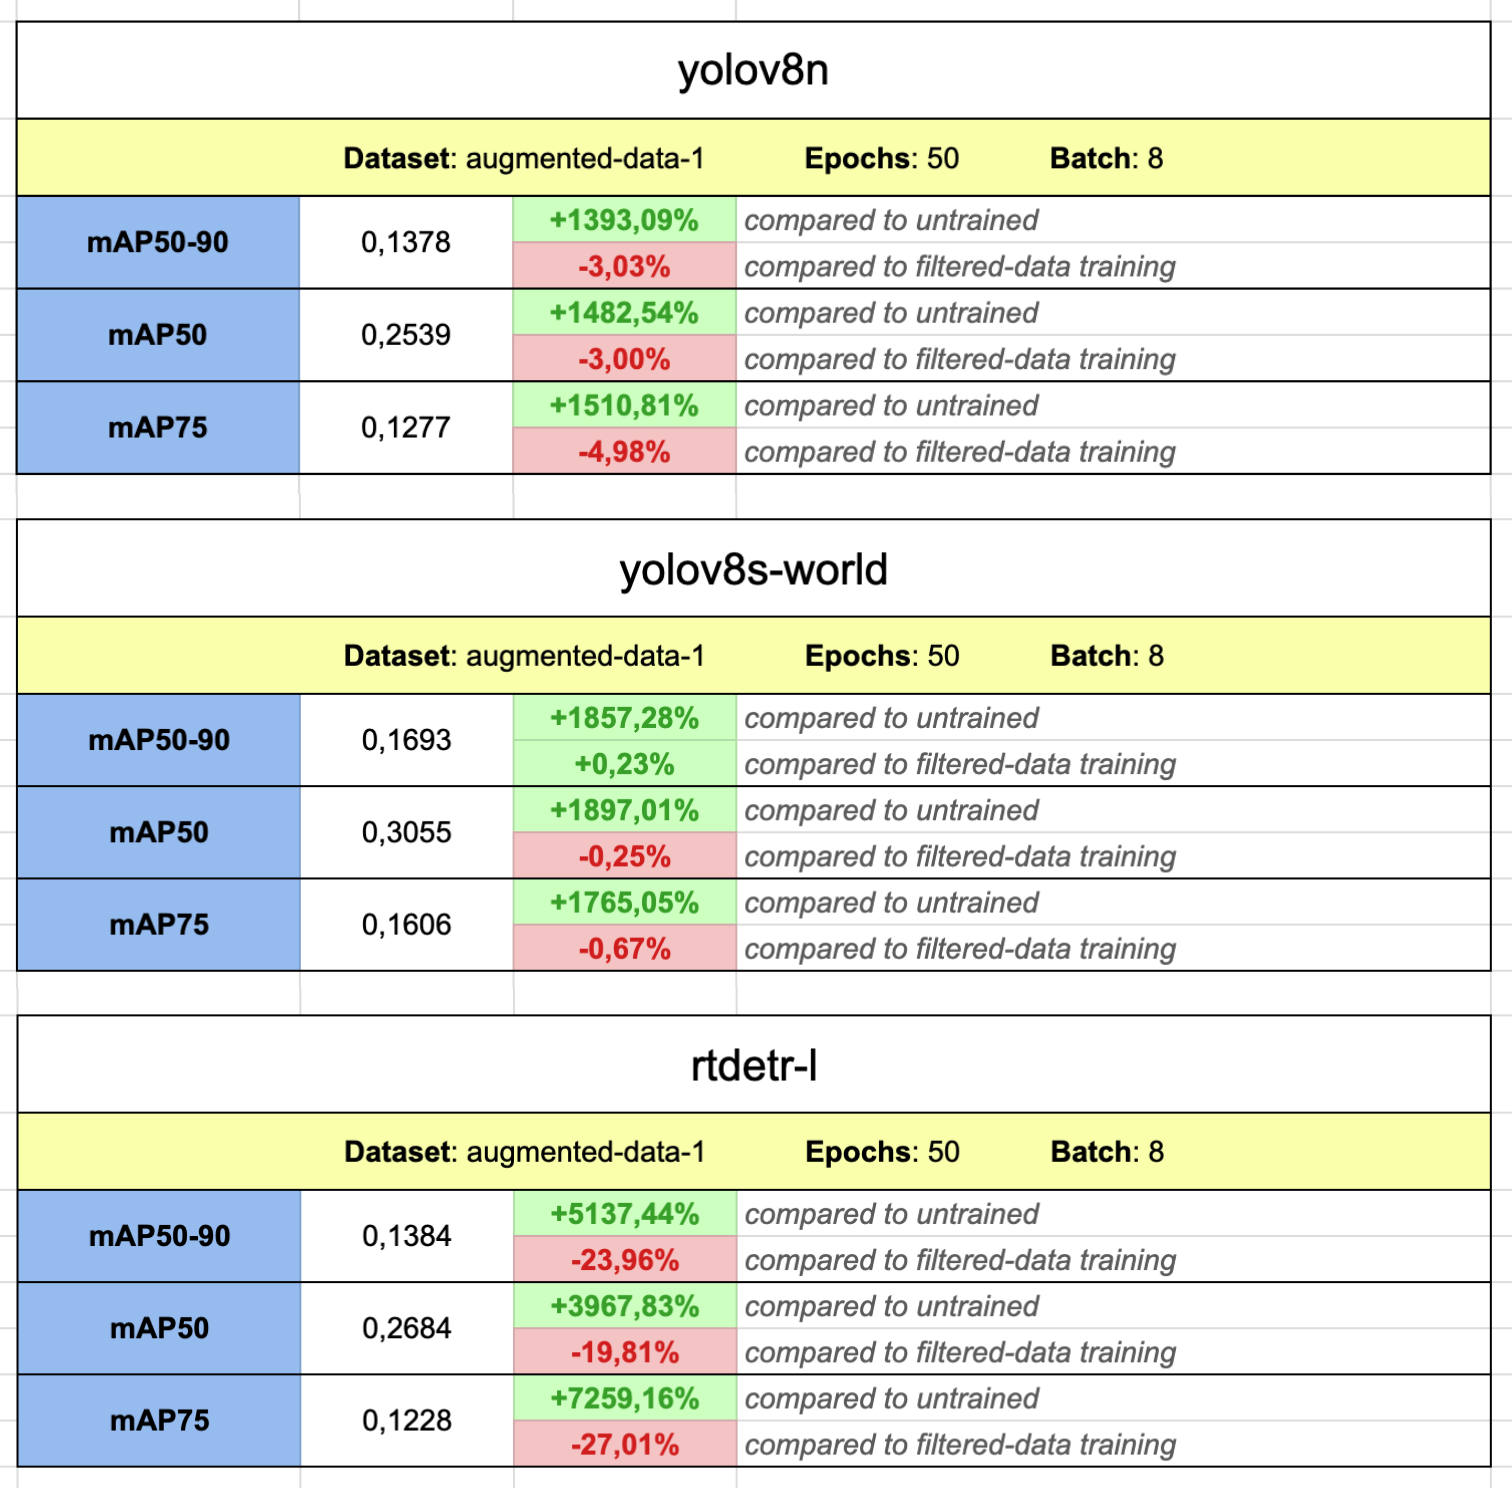
\includegraphics[width=0.9\textwidth]{files/capitoli/4-sperimentazione-risultati/assets/augmented-data-1-compare.png}
    \caption{\label{fig:augmented-data-1-compare}Confronto tra i risultati dei test dei modelli addestrati sul primo dataset aumentato e quelli dei precedenti test}
\end{figure}

\clearpage

\begin{figure}[ht]
    \centering
    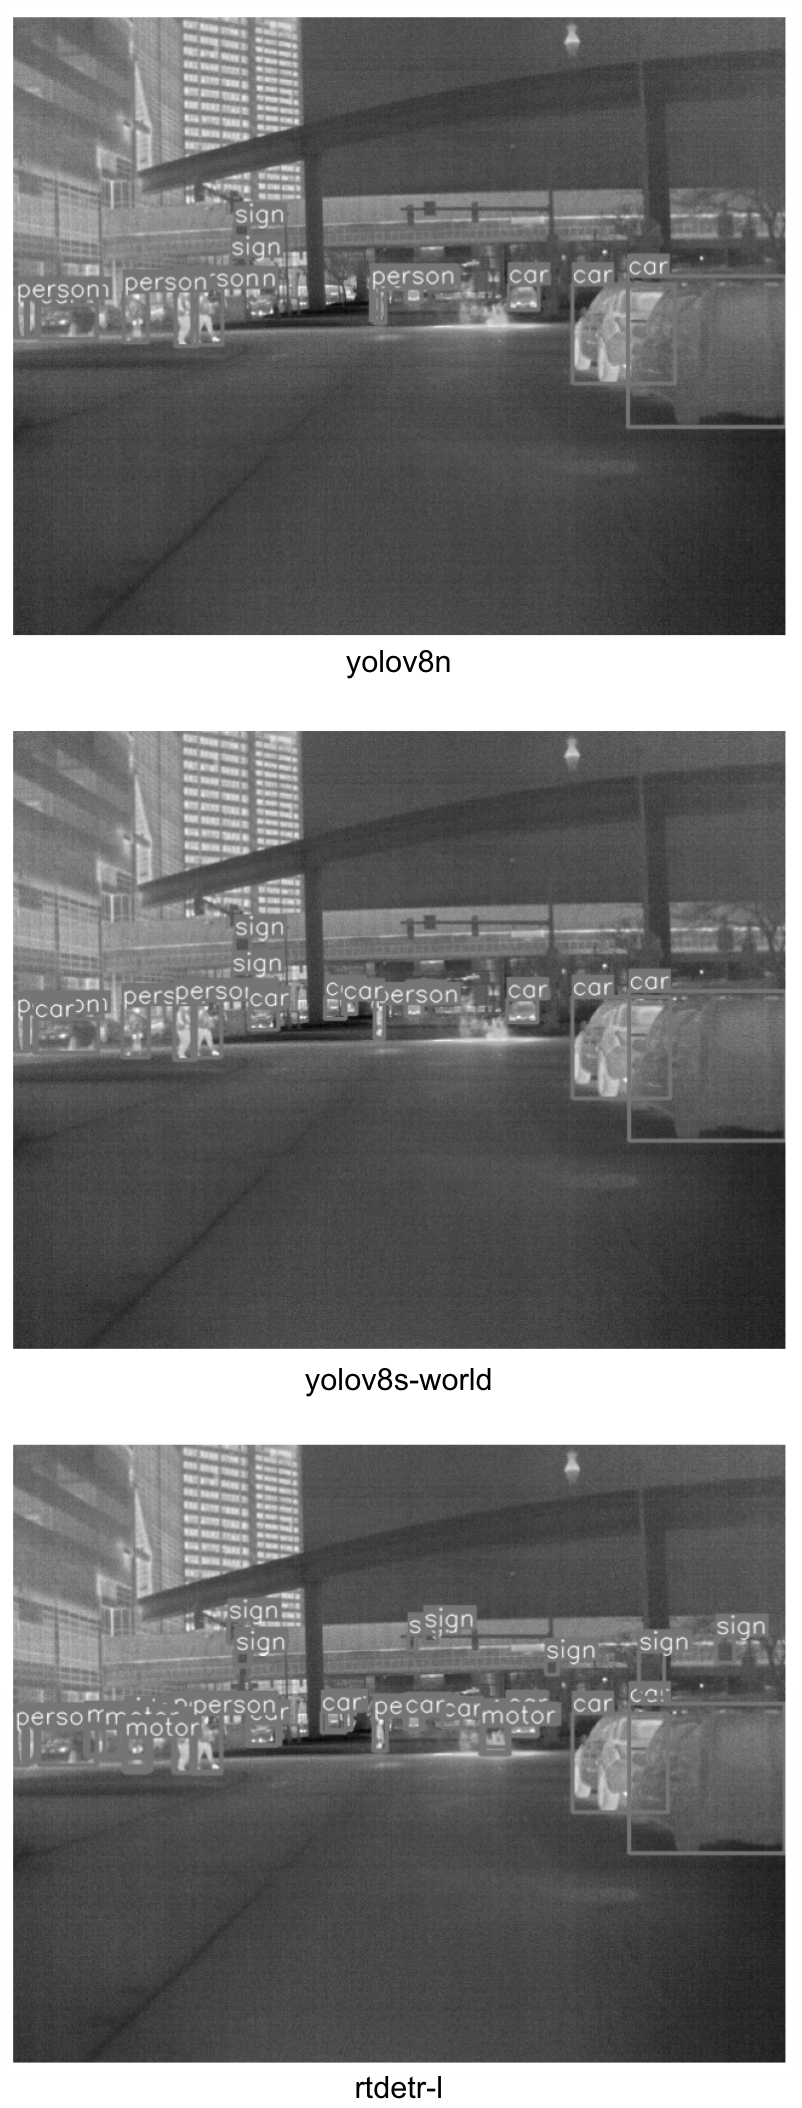
\includegraphics[width=0.6\textwidth]{files/capitoli/4-sperimentazione-risultati/assets/augmented-data-1-detections.png}
    \caption{\label{fig:augmented-data-1-detections}Detections effettutate dai modelli addestrati sul primo dataset aumentato}
\end{figure}

\clearpage

\subsection{Seconda Data Augmentation}

\subsubsection{Secondo dataset aumentato}
Visto il peggioramento delle prestazioni a seguito della prima data augmentation, sono andato a generare un secondo dataset aumentato tramite una nuova combinazione di trasformazioni mirata ad essere più coerente con il contesto delle immagini termiche:

\begin{figure}[ht]
    \centering
    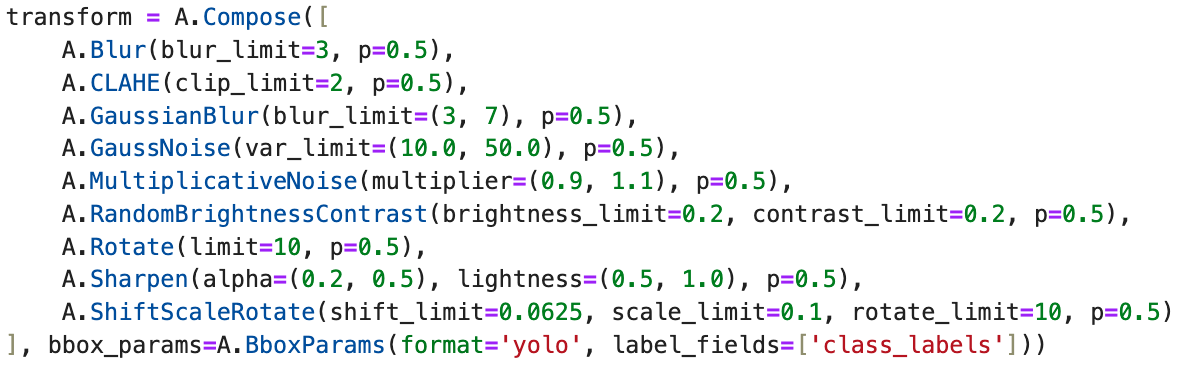
\includegraphics[width=0.9\textwidth]{files/capitoli/4-sperimentazione-risultati/assets/transform-2.png}
    \caption{\label{fig:transform-2}Definizione della nuova trasformazione di Albumentations da applicare alle immagini}
\end{figure}

Perciò, grazie allo stesso script Python utilizzato precedentemente, ho generato il dataset \texttt{augmented-data-2}.

% allungare descrivendo brevemente le trasformazioni scelte e come mai

\clearpage

\begin{figure}[ht]
    \centering
    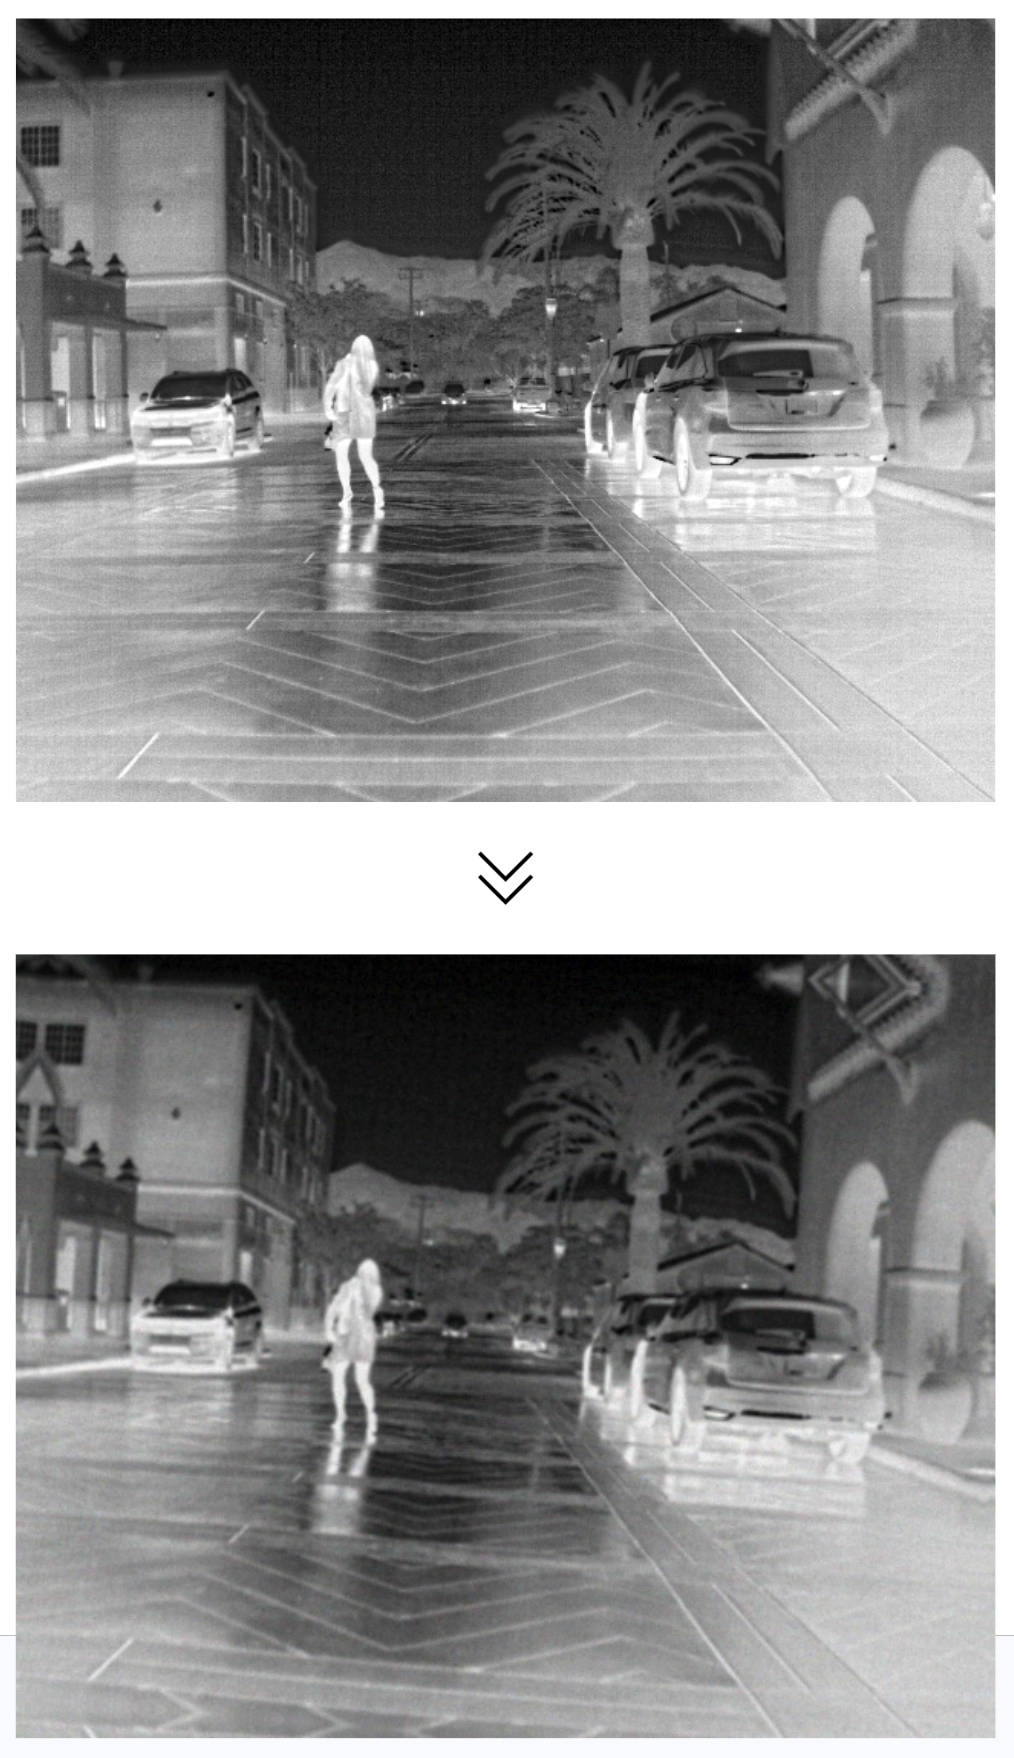
\includegraphics[width=0.8\textwidth]{files/capitoli/4-sperimentazione-risultati/assets/augmented-data-2-example.png}
    \caption{\label{fig:augmented-data-2-example}Esempio di immagine trasformata con la seconda data augmentation}
\end{figure}

\clearpage

\subsubsection{Test modelli addestrati sul secondo dataset aumentato}
A seguito del terzo addestramento, eseguito su \texttt{augmented-data-2} nelle medesime condizioni (50 epochs e batch size di 8), ho ottenuto i seguenti risultati dai test:

\begin{figure}[ht]
    \centering
    \includegraphics[width=1\textwidth]{files/capitoli/4-sperimentazione-risultati/assets/augmented-data-2-metrics.png}
    \caption{\label{fig:augmented-data-2-metrics}Risultati test dei modelli addestrati sul secondo dataset aumentato}
\end{figure}

Qua possiamo notare che i tre modelli si comportano diversamente: 

\begin{itemize}
    \item YOLOv8 ha un significativo miglioramento delle metriche rispetto ad entrambi gli addestramenti precedenti.
    \item YOLO-World ha un leggero incremento generale della mAP50-90 e della mAP50, mentre la mAP75 migliora rispetto a quella ottenuta a seguito dell fine-tuning con la prima data augmentation, ma rimane comunque inferiore a quella ottenuta con l'addestramento su dataset non aumentato.
    \item RT-DETR si comporta come nel precedente caso, mantendo tutte le metriche inferiori al primo addestramento su \texttt{filtered-data}, pur mostrando miglioramenti rispetto alla prima data augmentation.
    
\end{itemize}

\clearpage

\begin{figure}[ht]
    \centering
    \includegraphics[width=0.9\textwidth]{files/capitoli/4-sperimentazione-risultati/assets/augmented-data-2-compare.png}
    \caption{\label{fig:augmented-data-2-compare}Confronto tra i risultati dei test dei modelli addestrati sul secondo dataset aumentato e quelli dei precedenti test}
\end{figure}

\clearpage

\begin{figure}[ht]
    \centering
    \includegraphics[width=0.6\textwidth]{files/capitoli/4-sperimentazione-risultati/assets/augmented-data-2-detections.png}
    \caption{\label{fig:augmented-data-2-detections}Detections effettutate dai modelli addestrati sul secondo dataset aumentato}
\end{figure}

\clearpage

\subsubsection{Ulteriore addestramento sul secondo dataset aumentato}
Per confermare i risultati ottenuti nei test precedenti, ho effettuato un ulteriore addestramento sul dataset \texttt{augmented-data-2}, aumentando il numero di epochs a 100. I test effettuati al termine di esso hanno prodotto i seguenti risultati:

\begin{figure}[ht]
    \centering
    \includegraphics[width=1\textwidth]{files/capitoli/4-sperimentazione-risultati/assets/augmented-data-2(100)-metrics.png}
    \caption{\label{fig:augmented-data-2(100)-metrics}Risultati test dei modelli addestrati per 100 epochs sul secondo dataset aumentato}
\end{figure}

Dai risultati ottenuti possiamo osservare che:

\begin{itemize}
    \item YOLOv8 incrementa ulteriormente tutte le metriche di diversi punti percentuale rispetto ai precedenti addestramenti.
    \item YOLO-World incrementa tutte e tre le mAP, a differenza del precedente test in cui la mAP75 risultava inferiore a quella ottenuta con l'addestramento su \texttt{filtered-data}. Tuttavia, l'incremento è più contenuto rispetto a quello ottenuto con YOLOv8
    \item RT-DETR invece peggiora tutte le sue metriche rispetto al precedente addestramento di 50 epochs su \texttt{augmented-data-2}
\end{itemize}

\clearpage

\begin{figure}[ht]
    \centering
    \includegraphics[width=0.9\textwidth]{files/capitoli/4-sperimentazione-risultati/assets/augmented-data-2(100)-compare.png}
    \caption{\label{fig:augmented-data-2(100)-compare}Confronto tra i risultati dei test dei modelli addestrati per 100 epochs sul secondo dataset aumentato e quelli dei precedenti test}
\end{figure}

\clearpage

\begin{figure}[ht]
    \centering
    \includegraphics[width=0.6\textwidth]{files/capitoli/4-sperimentazione-risultati/assets/augmented-data-2(100)-detections.png}
    \caption{\label{fig:augmented-data-2(100)-detections}Detections effettutate dai modelli addestrati per 100 epochs sul secondo dataset aumentato}
\end{figure}

\clearpage
\section{Modello Ottimale}
Analizzando i risultati di tutte le sperimentazioni, possiamo evincere che YOLOv8 è il modello che ottiene il maggior incremento nelle prestazioni a seguito della data augmentation effettuata sul dataset termico. Fino a questo punto, abbiamo addestrato la versione "Nano" del modello; quindi per avere una visione più completa delle potenzialità di YOLOv8, ho deciso di addestrare la versione "Large" del modello (\textbf{yolov8l}\cite{27}) su \texttt{augmented-data-2}, mantenendo le 100 epochs. Seguono i risultati ottenuti dal test:

\begin{figure}[ht]
    \centering
    \includegraphics[width=0.5\textwidth]{files/capitoli/4-sperimentazione-risultati/assets/yolov8l-metrics.png}
    \caption{\label{fig:yolov8l-metrics}Risultati test di yolov8l addestrato per 100 epochs sul secondo dataset aumentato a confronto con le metriche ottenute da yolov8n con lo stesso addestramento}
\end{figure}

Notiamo che, a parità di addestramento, con la versione "Large" del modello riusciamo ad ottenere un ulteriore incremento di tutte le metriche rispetto a quelle ottenute dalla "Nano".

\clearpage

\begin{figure}[ht]
    \centering
    \includegraphics[width=1\textwidth]{files/capitoli/4-sperimentazione-risultati/assets/yolov8l-detections-special.png}
    \caption{\label{fig:yolov8l-detections}Detections effettutate da yolov8l addestrato per 100 epochs sul secondo dataset aumentato}
\end{figure}

\clearpage



%\chapter{Conclusioni}\label{ch:conclusioni}
\chapter*{Conclusioni}
\markboth{Conclusioni}{Conclusioni}
\addcontentsline{toc}{chapter}{Conclusioni}

A seguito degli esperimenti condotti, abbiamo osservato che tutti e tre i modelli (YOLOv8, YOLO-World e RT-DETR) hanno mostrato miglioramenti significativi nelle prestazioni quando sottoposti a un normale fine-tuning sul dataset termico. Tuttavia, un processo di data augmentation incoerente rispetto al dataset ha prodotto un generale abbassamento delle prestazioni, nonostante l'aumento della dimensione del subset di training.

Effettuando una data augmentation corretta e mirata per il dataset termico, solo YOLOv8 ha mostrato miglioramenti sostanziali, ragione per cui ritengo che la causa principale delle peggiori prestazioni di YOLO-World e RT-DETR sia la loro maggiore complessità, la quale potrebbe richiedere una gestione più sofisticata delle augmentations o una maggiore quantità di dati per ottenere miglioramenti significativi. Escludo che le performance inferiori dei due modelli siano dovute alle trasformazioni usate nella seconda data augmentation, in quanto si sarebbero dovuti manifestare peggioramenti anche nelle metriche di YOLOv8. 

Grazie ai risultati ottenuti con la versione "Nano" di YOLOv8, abbiamo determinato che l'ottava versione di YOLO è la tipologia di modello che meglio si adatta all'Object Detection di immagini termiche. Pertanto, ho addestrato la versione "Large" di YOLOv8, ottenendo così il modello ottimale per l'obiettivo che ci eravamo prefissati.

\addcontentsline{toc}{chapter}{Bibliografia}
\bibliographystyle{plain}
\bibliography{files/biblio}
%\bibliographystyle{unsrt}
%\bibliography{sp,xml}

\end{document} 